\documentclass{article}

\usepackage[english]{babel}
\usepackage[utf8]{inputenc}
\usepackage{hyperref}
\usepackage{amsmath}
\usepackage{amssymb}
\usepackage{multirow}
\usepackage{booktabs}
\usepackage{longtable}
\usepackage[labelfont=bf]{caption}
\DeclareCaptionFormat{myformat}{#1#2#3\hrulefill}
%\captionsetup[figure]{format=myformat}
\usepackage{tikz}
\usepackage{subfigure}
\usepackage{geometry}
\usepackage{ifthen}

\usepackage{titlesec}
\titleformat
{\part}
[display]
{\bfseries\LARGE}
{}
{-2ex}
{\MakeUppercase{\partname{ }}\thepart:{ }}
[\vspace{.5ex}%
]


\usepackage{cite}

\usetikzlibrary{decorations.pathmorphing}

\bibliographystyle{plain}

\geometry{margin=3.5cm, bottom=2cm, top=2cm}

\newcommand{\todo}[2][]{\textcolor{red}{TODO\ifthenelse{\equal{#1}{}}{}{[#1]}: #2}}
\newcommand{\done}[2][]{\textcolor{green!50!black}{Done\ifthenelse{\equal{#1}{}}{}{[#1]}: #2}}
%\newcommand{\todo}[1]{}
\newcommand{\korrektur}[1]{\textcolor{red}{\textbf{Korrektur:} #1}}
\newcommand{\reals}{\mathbb{R}}

\newcommand{\zoomfactor}{0.5}
\newcommand{\autozoomfactor}{0.15}

\newcommand{\figurepage}[1]{
  %\newgeometry{top=0cm, bottom=0cm}
  \input{#1}
  %\restoregeometry
}

% for me, this looks better. uncomment these lines if you do not like it that small
%\renewcommand{\zoomfactor}{0.3}
%\renewcommand{\autozoomfactor}{0.075}

\title{Some aspects regarding shallow water equations in connection with the Lax-Friedrich-Flux}
\author{Stjepan Bakrac \and Philipp M\"uller}
\date{}

\newcommand{\partialderivative}[1]{\dfrac{\partial}{\partial #1}}
\newcommand{\pd}[2]{\dfrac{\partial #1}{\partial #2}}
\newcommand{\totalderivative}[1]{\dfrac{d}{d #1}}
\newcommand{\naturals}{\mathbb{N}}

\renewcommand{\phi}{\varphi}

\newcommand\intend{\mathrm{d}}

\DeclareMathOperator{\divergence}{div}

\begin{document}

\maketitle{}

\todo{Before submission, run
  \begin{center}
    \texttt{grep -nri 'todo' . --include=*.tex}
  \end{center}
and see if all todo's are done}

\todo{plots weiter stauchen}

\todo{Kantenintegration: Woher haben wir die Nullstellen - Referenz?}

\todo{Referenzen: Lax-Fridrichs-Löser (Leveque) -- Höhere Ordnung (Castro) -- Eulergleichungen (Cockburn/Geraldo(?)) -- Nodale Basis (Hesthaven)}

\todo{Sollten wir langsam ein Inhaltsverzeichnis reinhauen?}

\begin{abstract}
  The question how to simulate waves on a computer is subject to many difficulties. At several points in the process approximations have to be made to be feasibly computable. One of those points is the discretization of the continuous space into finite segments, usually triangles. Another is the simulation of the domain of each segment by sampling specific points within that segment. Yet another point is not as obvious, and occurs when trying to calculate a complex integral. The complexity is of such degree that it is usually not feasible to compute exactly, and for that another approximation has to be made.

  Despite all of this, the accuracy loss can normally be minized by sacrificing computing time. However, the specific approximation of an integrated fractional function using Gaussian quadrature has to be analyzed separately. It occurs when calculating how much of the relevant quantities are passed from one segment to another, which, due discontinuities along the separating lines, has to be handled in a way that preserves as much accuracy as possible.

  This paper aims to explain the derivation of the necessary equations for calculating those quantities, and goes into detail about comparing the analytical solution to the approximate solution using Gaussian quadrature.
\end{abstract}

\part{Deriving necessary equations}
\label{part:introduction}

\section{Problem statement}
\label{sec:problem-statement}

We want to simulate wave propagation along a certain area. There are several equations, suited for different situations, that deal with those kind of problems. The main problem for computer simulation is that the entire domain has to be discretized, usually in sets of triangles that all contain several fields of information (such as mass/height, velocity, etc.). But even without discretization problems, accurately simulating wave propagation is a challenging task, because several of the involved factors are very hard to calculate. Especially in tsunami-related environments even non-local factors like bathymetry information, tidal forces and the coriolis effect have to be considered to get accurate results.

In this documentation we will focus mainly on the derivation of the shallow water equations, which serve as a starting point for calculating wave propagation, along with an analysis of the discretization problem, as well as numerical solutions for it.

\section{Adaptive triangle grid}
\label{sec:triangles}

For our purposes we use an adaptive triangle grid. In areas with many variations, the grid adapts to a finer resolution, allowing for more detailed calculations, while not wasting unnecessary computation time in areas with lower variation.

Using this scheme, we can simplify a few steps in the calculation process. With a suitable library for coordinate projection, we can rotate triangles and edges into a space that's relevant for us. So instead of having to adjust how we apply the functions, based on which edges the triangles are touching on (because different edges suggest different positions in space), we just rotate the triangles into a certain space, so we only need to consider this space when applying funtions and algorithms.

In addition to rotating, we can also scale the edges of the triangles to always be in a certain shape. We'll use that to scale the catheses to length 1 and hence the hypothenuse to length $\sqrt{2}$. This will help with further calculations, because some of them will rely on the length of an edge, which can be conveniently omitted (or set to the constant $\sqrt{2}$ respectively).

\begin{figure}[ht]
  \centering
  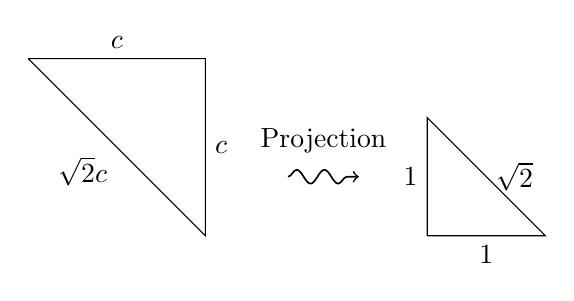
\begin{tikzpicture}[scale=1.5]
    \draw (-2.5,1.5) -- node[above]{$c$} (-1,1.5) -- node[right]{$c$} (-1,0) -- node[below left]{$\sqrt{2}c$} (-2.5,1.5);
    \draw[->,semithick,decorate,decoration=snake] (-0.3,0.5) -- node[above,yshift=.5em]{Projection} (0.3,0.5);
    \begin{scope}[xshift=2.5em]
      \draw (0,0) -- node[left]{1} (0,1) -- node[right]{$\sqrt{2}$} (1,0) -- node[below]{1} (0,0);
    \end{scope}

  \end{tikzpicture}
  \caption{A sample triangle rotated into normal space and scaled down to cathetus length 1.}
  \label{fig:triangle-projection}
\end{figure}

For further reference, we will be calling the domain of the entire triangle $T$ (the set of all points on the triangle), and the set of edges $E$, enumerated with $e_i$, $\forall i \in {1,2,3}$. Points on the triangle (both on the edge and inside) will be denoted by $p$. In the implementation we will be referring to the edges \texttt{left}, \texttt{hyp} and \texttt{right} by $e_1$, $e_2$ and $e_3$ respectively.

\begin{figure}[ht]
  \centering
  \subfigure[Degree 0]{
    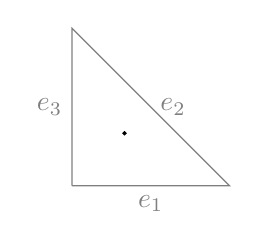
\begin{tikzpicture}[scale=2]
      \draw[opacity=0.5] (0,0) -- node[left]{$e_3$} (0,1) -- node[right]{$e_2$} (1,0) -- node[below]{$e_1$} (0,0);
      \draw[fill=black] (0.33333333, 0.3333333333) circle (0.01);
    \end{tikzpicture}
  }
  \subfigure[Degree 1]{
    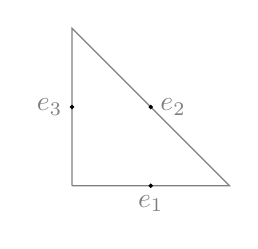
\begin{tikzpicture}[scale=2]
      \draw[opacity=0.5] (0,0) -- node[left]{$e_3$} (0,1) -- node[right]{$e_2$} (1,0) -- node[below]{$e_1$} (0,0);
      \draw[fill=black] (0.5, 0) circle (0.01);
      \draw[fill=black] (0, 0.5) circle (0.01);
      \draw[fill=black] (0.5, 0.5) circle (0.01);
    \end{tikzpicture}
  }
  \subfigure[Degree 2]{
    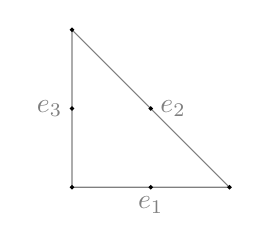
\begin{tikzpicture}[scale=2]
      \draw[opacity=0.5] (0,0) -- node[left]{$e_3$} (0,1) -- node[right]{$e_2$} (1,0) -- node[below]{$e_1$} (0,0);
      \draw[fill=black] (0.5, 0) circle (0.01);
      \draw[fill=black] (0, 0.5) circle (0.01);
      \draw[fill=black] (0.5, 0.5) circle (0.01);
      \draw[fill=black] (0, 0) circle (0.01);
      \draw[fill=black] (1, 0) circle (0.01);
      \draw[fill=black] (0, 1) circle (0.01);
    \end{tikzpicture}
  }
  \subfigure[Degree 3]{
    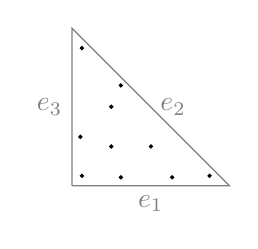
\begin{tikzpicture}[scale=2]
      \draw[opacity=0.5] (0,0) -- node[left]{$e_3$} (0,1) -- node[right]{$e_2$} (1,0) -- node[below]{$e_1$} (0,0);
      \draw[fill=black] (0.501426509658179, 0.24928674517091) circle (0.01);
      \draw[fill=black] (0.24928674517091, 0.24928674517091) circle (0.01);
      \draw[fill=black] (0.24928674517091, 0.501426509658179) circle (0.01);
      \draw[fill=black] (0.873821971016996, 0.063089014491502) circle (0.01);
      \draw[fill=black] (0.063089014491502, 0.063089014491502) circle (0.01);
      \draw[fill=black] (0.063089014491502, 0.873821971016996) circle (0.01);
      \draw[fill=black] (0.053145049844817, 0.310352451033784) circle (0.01);
      \draw[fill=black] (0.310352451033784, 0.636502499121399) circle (0.01);
      \draw[fill=black] (0.636502499121399, 0.053145049844817) circle (0.01);
      \draw[fill=black] (0.310352451033784, 0.053145049844817) circle (0.01);
    \end{tikzpicture}
  }
  \caption{Triangles containing a support points for polynomial degrees 0 through 3.}
  \label{fig:triangle-support-points-var-degrees}
\end{figure}

The points in the triangle are support points. The number depends on the degree of the test functions, as will be discussed in section \ref{sec:basis-functions-choice}. As it is impossible to calculate the propagation exactly, we need to find a numerical approximation. This will be done with the discontinuous Galerkin method explained in section \ref{sec:discontinuous-galerkin}. However, for each test function used for the method we will need one point in the triangle to save the calculated information to. They can be regarded as sample points that are representative for the values within the triangle. The higher polynomial degree we operate on, the more support points we will have. While this increases accuracy, it has a negative impact on efficiency, so a proper balance is desired.

Another set of points are \emph{Gaussian quadrature} points, which we will use later on to approximate integrals along the edges. Accordingly, they will also be located on the respective edges. They will be explained in more detail in section \ref{sec:boundary-integral}.

\section{Choice of basis functions}
\label{sec:basis-functions-choice}

For our project, we restricted ourselves to polynomial basis functions (depending on two variables $x$ and $y$) of variable degree $d$. The name already gives away the nature of these functions, because they are supposed to be bases for a polynomial space, so that we can construct any polynomial of degree $d$ as a linear combination of these basis functions.

A relatively simple way of constructing basis functions is to use Lagrange interpolation:
\begin{itemize}
\item Choose a certain set of $n$ points $p_1$ through $p_n$ (see \ref{sec:choice-support-points}).
\item Construct function $\phi_i$ such that $\phi_i(p_j) = \delta_{ij} \  \forall i,j \in \{1 \dots n\}$ using Lagrange polynomials (with $\delta_{ij}$ being the Kronecker delta function).
\end{itemize}

The (minimum) number of basis functions $n$ is not arbitrary, but it depends on the degree of the polynomials. If we only employ polynomials of degree 0 (i.e.\,constants), we only need one basis function. Increasing the degree by 1 involves introducing variables $x$ and $y$. Thus, we need three polynomials to construct every polynomial of degree 1, one to create polynomials containing $x$, one to create polynomials containing $y$ and one to create other constant polynomials.

Generalizing this scheme we observe the following: if we want to use polynomials of degree $d$, a polynomial can contain terms $x^a y^b$ with $a+b \leq d$. A simple combinatorial arguments indicates that we need $\frac{(d+2) \cdot (d+1)}{2}$ basis functions to span the function space containing all the polynomials up to degree $d$.

\subsection{Choice of support points}
\label{sec:choice-support-points}

As mentioned before, we construct the basis functions with the help of some support points. However, arbitrary choosing those can lead to accuracy loss in the best case, and malconditioned matrices, which can prevent precomputing arrays in the worst.

For low degree polynomials, we choose specific distribution of the support points within the triangle:
\begin{description}
\item[Degree 0] We choose the support point at the center of the triangle (at $\left(\frac{1}{3}, \frac{1}{3}\right)$).
\item[Degree 1] We choose the support points at the center of each edge.
\item[Degree 2] We choose the support points at the triangle corners and at the center of each edge.
\end{description}

For higher degree, we choose the points derived by Dunavant (see \cite{dunavant1985high}). The distributions of support points are illustrated in figure \ref{fig:triangle-support-points-var-degrees}.

\subsection{Summary: Basis functions for low degrees}
\label{sec:basis-functions-for-low-degrees}

To have an impression of what the basis functions look like, please have a look at table \ref{tab:basis-functions-for-low-degrees}. It shows the basis functions for orders 0 to 2.

\begin{table}[ht]
  \centering
  \begin{tabular}{cclll}
    \toprule
    Order & $n$ & Basis functions & $x$-derivative & $y$-derivative \\
    \midrule
    \multirow{1}{*}{0} & 1 & 1 \\
    \midrule
    \multirow{3}{*}{1} & \multirow{3}{*}{3} & $1-2y$ & 0 & -2\\
    &  & $-1+2x+2y$ & 2 & 2\\
    &  & $1-2x$ & -2 & 0\\
    \midrule
    \multirow{6}{*}{2} & \multirow{6}{*}{6} & $1-3\,x-3\,y+2\,{x}^{2}+4\,xy+2\,{y}^{2}$ & $-3+4x+4y$ & $-3+4x+4y$\\
& & $4\,x-4\,{x}^{2}-4\,xy$ & $4-8x-4y$ & $-4x$\\
& & $-x+2\,{x}^{2}$ & $-1+4x$ & 0\\
& & $4\,xy$ & $4y$ & $4x$\\
& & $-y+2\,{y}^{2}$ & $0$ & $-1+4y$\\
& & $4\,y-4\,xy-4\,{y}^{2}$ & $-4y$ & $4-4x-8y$ \\
    \bottomrule
  \end{tabular}
  \caption{Basis functions for low degree. Note that these basis functions are not the only possible choosings. We, however, will focus on them throughout this text. The second column ($n$) denotes the number of basis functions used for the respective order.}
  \label{tab:basis-functions-for-low-degrees}
\end{table}

\subsubsection{Symmetry in basis function}
\label{sec:basis-function-symmetry}

If you consider table \ref{tab:basis-functions-for-low-degrees}, you'll recognize that there are some symmetries for the basis functions. We will point out some of these symmetries here because they will make our lives easier later.

\paragraph{Order 1}

For order 1, we see that the third and the first basis function look somewhat similar. To be precise, we recognize that $\phi_1(x,y)=\phi_3(y,x)$. This symmetry -- of course -- also holds for the respective derivatives.

\paragraph{Order 2}

For second order, the thing involves a bit more elaboration, but is still easy. We obtain that $\phi_2(x,y)=\phi_6(y,x)$ and $\phi_3(x,y)=\phi_5(y,x)$. The basis functions $\phi_1$ and $\phi_4$ can be interpreted to be ``symmetric to themselves'': $\phi_1(x,y)=\phi_1(y,x)$ and $\phi_4(x,y)=\phi_4(y,x)$.

\subsubsection{Other properties}
\label{sec:basis-functions-other-properties}

We conjecture the following two identities: \todo[Philipp]{Stimmen die von mir angeführten Beweise/Erklärungen?}

\begin{align}
  \label{eq:sum-basis-functions-is-1}
  \sum_{i=1}^n \phi_i(x,y) &= 1 \\
  \left( \sum_{i=1}^n a \cdot \phi_i(x,y) \right)^2 &= a^2
\end{align}

We verified these two equations for first and second order using maple (and generic support points). However, we do not know how to prove them by hand and generalized for higher orders. While these two may look a bit farfetched at first, they will later be useful when we examine specific plots.

The second equation can be easily followed from the first one.

The first equation can be derived the following way: If we have basis functions $\phi_1$ to $\phi_n$, o a certain orer (say order $o$ --- which implies $n=\frac{(o+1)(o+2)}{2}$). If we then take the sum $\sum_{i=1}^n \phi_i(x,y)$ we obtain a polynomial of degree $o$. This polynomial has exactly $n$ coefficients that may be obtained by solving a system of linear equations containing $n$ equations These equations are obtained using the $n$ support points, i.e. we have a system of $n$ equations and $n$ coefficients which -- on the other hand -- means, that all the coefficients are determined uniquely (if the system of equations can be solved).

Note that for any support point $(x_p,y_p)$, we have that

\begin{equation}
  \sum_{i=1}^n \phi_i(x_p,y_p) = 1
\end{equation}

Moreover, we know that the polynomial $\overline{\rho}(x,y)=1$ is a polynomial that fulfils $\overline{\rho}(x_p,y_p)$ for all support points $(x_p,y_p)$. Since the coefficients for the polynomial are uniquely determined we know that $\sum_{i=1}^n \phi_i(x,y)$ must be the same as $\rho$. Thus, we can conclude equation (\ref{eq:sum-basis-functions-is-1}).

\section{Discontinuous Galerkin}
\label{sec:discontinuous-galerkin}

The numerical method we are using to solve the shallow water equations on our grid is the discontinuous Galerkin method (DG). It combines ideas from the finite element method and the finite volume method. The first suggests computing solutions for each element locally, which is what the DG method also does. However, it lets adjacent elements communicate relevant information with each other by numerically calculating a flux function, which determines how much of each stored quantity is passed along between elements, which is a method borrowed from finite volume schemes. We can apply this to the general continuity equation, which looks like this in its differential form:

\begin{equation}
  \label{eq:general-continuity-equation}
  \pd{\mathbf{q}}{t} + \nabla \cdot F(\mathbf{q}) = r
\end{equation}

\begin{itemize}
\item[$\mathbf{q}$] The state vector, containing all relevant information for any given point in space.
\item[$F$] The flux function, applied to $\mathbf{q}$ it results in a vector describing the spatial transport of the quantities stored in $\mathbf{q}$.
\item[$r$] A source term, which is used to offset the calculated quantities. What this quantity means can differ depending on the situation.
\end{itemize}

Similar to the finite element method, we multiply the equation by a test function, then integrate over the entire domain. This can be done with more than one function as well, and we will use several, depending on the degree of the functions we use. These functions happen to be the basis functions we mentioned in section \ref{sec:basis-functions-choice}. Essentially, what we obtain is the following (with $\phi_i$ being the basis function):

\begin{equation}
  \label{eq:general-continuity-equation-discontinuous-galerkin}
  \int_\Omega \pd{\mathbf{q}}{t} \phi_i \,d\Omega + \int_\Omega \nabla \cdot F(\mathbf{q}) \phi_i \,d\Omega = \int_\Omega r \phi \,d\Omega
\end{equation}

We will later use this to transform the shallow water equations into a different form which is easier to compute.

\section{Shallow water equations}
\label{sec:shallow-water-equations}

The shallow water equations can be applied to the general continuity equation by choosig appropriate variables. For the state vector $\mathbf{q}$ we use the following:

\begin{eqnarray*}
  \mathbf{q} =
  \begin{pmatrix}
    h \\ h v_x \\ h v_y
  \end{pmatrix}
\end{eqnarray*}

Here $h$ is the height of the water at that point, which is proportional to the mass. $v_x$ and $v_y$ are the velocities in the $x$ and $y$ direction. Note that we will occasionally use $\mathbf{v}$, which means a two-dimensional vector consisting of $\begin{pmatrix} v_x \\ v_y \end{pmatrix}$. Next, the flux function can be defined like so:

\begin{eqnarray*}
  F(\mathbf{q}) =
  \begin{pmatrix}
    h \mathbf{v} \\ h v_x \mathbf{v} + \frac{1}{2} g h^2 e_x \\ h v_y \mathbf{v} + \frac{1}{2} g h^2 e_y
  \end{pmatrix}
\end{eqnarray*}

This takes into account gravitic effects for the respective $x$ and $y$ components. This is accomplished by $e_x$ and $e_y$, which are $\begin{pmatrix} 1 \\ 0 \end{pmatrix}$ and $\begin{pmatrix} 0 \\ 1 \end{pmatrix}$ respectively, thus only adding the gravitational terms where necessary.

As for the source term, we can interpret it to be the bathymetry in our case, to offset our calculated results from the state and flux function. For simplicity, we will use $r=
\begin{pmatrix}
  0 \\ 0\\ 0
\end{pmatrix}$ (i.e.\,assuming constant even bathymetry).

Having defined those terms to suit our purpose, we can rewrite the above as follows:

\begin{eqnarray}
  \label{eqn:shallow-water-flux}
  \mathbf{q} =
  \begin{pmatrix}
    h \\ u_x \\ u_y
  \end{pmatrix} \quad
  F(\mathbf{q}) =
  \begin{pmatrix}
    \mathbf{u} \\ \frac{u_x}{h}\mathbf{u} + \frac{1}{2} g h^2 e_x \\ \frac{u_y}{h}\mathbf{u} + \frac{1}{2} g h^2 e_y
  \end{pmatrix}
\end{eqnarray}

Here we replaced the velocity $\mathbf{v}$ by the momentum $\mathbf{u}$, which, similarly, consists of two dimensions, one in each direction (referred to by $u_x$ and $u_y$). Occasionally we will need only the $x$ components (or $y$ components) from that vector, for which we will write $F^x$ (and $F^y$ respectively):

\begin{eqnarray*}
  F^x(\mathbf{q}) =
  \begin{pmatrix}
    u_x \\ \frac{u_x^2}{h} + \frac{1}{2} g h^2 \\ \frac{u_x u_y}{h}
  \end{pmatrix}
  \quad
  F^y(\mathbf{q}) =
  \begin{pmatrix}
    u_y \\ \frac{u_x u_y}{h} \\ \frac{u_y^2}{h} + \frac{1}{2} g h^2
  \end{pmatrix}
\end{eqnarray*}

At this point we apply the discontinuous Galerkin method as mentioned above. We obtain the following, called the weak form:

\begin{equation}
  \label{eq:shallow-water-weak-form}
  \int_T \pd{\mathbf{q}}{t} \phi \,dT + \int_T \nabla \cdot F(\mathbf{u}) \phi \,dT = 0
\end{equation}

The operator $\nabla \cdot$ is the divergence, which computes the sum of the $x$ derivative of the first component and the $y$ derivative of the second component. Using the operator $\nabla$ and applying the Gaussian divergence theorem, we can transform the above into the following set of equations:

\begin{equation}
  \label{eq:shallow-water-weak-form-div-applied}
  \int_T \pd {\mathbf{q}}{t} \phi \, dT +
  \int_{\partial T} F(\mathbf{q}) \cdot \mathbf{n} \, \phi \, ds -
  \int_T F(\mathbf{q}) \cdot \nabla \phi \, dT = 0
\end{equation}

Note at this point, that these are actually six equations, one for each component of $\mathbf{q}$, each of which contains two-dimensional vectors for the two space coordinates. The dot product here signifies a scalar product, i.e.\,multiply the components by row and add up the result. The last integral contains the symbol $\nabla$. This operator takes a function and creates a vector from it containing the derivatives for $x$ and $y$ in the respective components.

The second integral in that equation is a boundary integral around our triangle. The $\mathbf{n}$ in there denotes the (outward facing) normal at that point. We write $ds$ to denote integration over the $(x,y)$ values along the border. Since it is a boundary integral of a triangle, we can split it up into three integrals (one for each edge of the triangle), which will aid in computation of the term. This also implies splitting the normal vector $\mathbf{n}$ into three vectors, one for each edge. This helps as well, because the normal vector is constant within each edge.

\begin{equation}
  \label{eq:boundary-integral-sum}
  \int_{\partial T} F(\mathbf{q}) \cdot \mathbf{n} \, \phi \, ds = \sum_{e \in E} \int_{e} F(\mathbf{q}) \cdot \mathbf{n}_e \, \phi \, ds = \sum_{e \in E} \int_{e} F^e \phi \, ds =: \text{Boundary integral}
\end{equation}

We also combined the terms $F(\mathbf{q})$ and $\mathbf{n}$ to one term $F^e$. This term denotes the quantities given or received from the triangle neighboring on the edge $e$. The normal will not pose a problem for us, as we rotate the edges into a standardized space, so they can all be computed the same way, regardless of position (this process is described in section \ref{sec:triangles}). As was mentioned in \ref{sec:discontinuous-galerkin}, we apply this method for every basis function at our disposal. Since we have one for each support point, it will run from 1 through $n$, named $\phi_i$ accordingly:

\begin{equation}
  \label{eq:shallow-water-weak-form-div-applied-approximation}
  \int_T \pd {\mathbf{q}}{t} \phi_i \, dT +
  \sum_{e \in E} \int_{e} F^e \phi_i \, ds  -
  \int_T F(\mathbf{q}) \cdot \nabla \phi_i \, dT = 0
  \quad \forall i \in {1 \dots n}
\end{equation}

\section{Matrix extraction}
\label{sec:matrix-extraction}

Equation \ref{eq:shallow-water-weak-form-div-applied-approximation} gives a lot of room to improve regarding efficiency. Upon closer examination, some terms stand out as being constant, or independent of the values at specific points, which means we can extract them and precompute them to save computation time while the program is running. For that, we will try to extract as much information as possible into matrices.

To do that, we first have to get rid of the various terms containing $\mathbf{q}$. Since $\mathbf{q}$ depends on the position, and that is what we integrate over, we cannot extract it from the integral. To achieve this regardless, we use the following approximation over all support points and corresponding basis functions:

\begin{equation}
  \label{eq:support-point-approximation}
  \mathbf{q} \approx \sum_{i=1}^n \mathbf{q}_i \phi_i\left(x,y\right)
\end{equation}

$\mathbf{q}_i$ are the $\mathbf{q}$-values at the corresponding support points. Since those do not depend on the position, it allows us to move them out of the integral, leaving integrals over various combinations of basis functions, which are all independant of $\mathbf{q}$, and hence can be precomputed.

Please note that $\mathbf{q}$ (and all $\mathbf{q}_i$) contain three components: The height $h$, the momentum in $x$-direction $u_x$ and the $y$ momentum $u_y$. This means, equation (\ref{eq:support-point-approximation}) yields three equations (one for each of the components).

\subsection{Mass matrix}
\label{sec:mass-matrix}

The first integral of (\ref{eq:shallow-water-weak-form-div-applied-approximation}) shows exactly how this works. As only the basis functions $\phi_i$ are dependent on $(x,y)$, we can extract $\mathbf{q}$ and obtain a constant term:

\begin{eqnarray*}
  \int_T \pd {\mathbf{q}}{t} \phi_i \, dT & \approx &
  \int_T \pd {\left( \sum_{j=1}^n \mathbf{q}_j \phi_j \right) }{t} \phi_i \, dT = \\
  & = & \sum_{j=1}^n \underbrace{\int_T \phi_i \phi_j \, dT}_{m_{ij}} \pd{\mathbf{q}_j}{t}
\end{eqnarray*}

The elements $m_{ij}$ form the $n \times n$ mass matrix $M$. That means we have a product between $M$ and a vector containing all $\mathbf{q}$ components differentiated by $t$. For a shorthand notation, we can define $\tilde{\mathbf{q}} := \begin{pmatrix} \mathbf{q}_1 \\ \vdots \\ \mathbf{q}_n \end{pmatrix}$. Using this, we can now translate the above into the following formula:

\begin{equation*}
  \int_T \pd {\mathbf{q}}{t} \phi_i \, dT \approx
  M \cdot \pd{
    \tilde{\mathbf{q}}}{t}
\end{equation*}

\subsection{Stiffness matrix}
\label{sec:stiffness-matrix}

We will skip the second integral for now and move to the third. We need to treat each of the three components differently. In this section we will see the state vector array splitting up by their coordinates and giving us different results for the $x$ and $y$ components. This means we will be using the $F^x\left(\mathbf{q}\right)$ and $F^y\left(\mathbf{q}\right)$ terms defined in \ref{sec:shallow-water-equations} for simpler notation.

Before we go on, let us recapitulate some notation:
\begin{itemize}
\item $\phi_j$ is the $j$-th basis function ($j$ ranging from 1 to $n$)
\item $u_{x,j}$ denotes the weight for basis function $\phi_j$ in the approximation of $u_x$
\item $u_{y,j}$ -- similar to $u_{x,j}$
\item $h_j$ denotes the weight for basis function $\phi_j$ in the approximation of $h$
\end{itemize}

\subsubsection{First line}
\label{sec:stiffness-matrix-first-line}

Using the same method as in \ref{sec:mass-matrix}, we obtain:

\begin{eqnarray*}
  \int_T F_1(\mathbf{q}) \cdot \nabla \phi \, dT & = &
  \int_T
  \begin{pmatrix}
    u_x \\ u_y
  \end{pmatrix}
  \cdot \nabla \phi_i \, dT \approx \\
  &=& \int_T
  \begin{pmatrix}
    \sum_{j=1}^n u_{x,j} \phi_j \\
    \sum_{j=1}^n u_{y,j} \phi_j \\
  \end{pmatrix}
  \cdot
  \begin{pmatrix}
    \pd{\phi_i}{x} \\
    \pd{\phi_i}{y}
  \end{pmatrix} dT \\
  & = & \sum_{j=1}^n u_{x,j} \underbrace{\int_T \phi_j \pd{\phi_i}{x} \, dT}_{s_{ij}^x} + \sum_{j=1}^n u_{y,j} \underbrace{\int_T \phi_j \pd{\phi_i}{y} \, dT}_{s_{ij}^y}
\end{eqnarray*}

Again we obtain matrices, denoted by the elements $s_{ij}^x$ and $s_{ij}^y$, stored in $S^x$ and $S^y$ respectively (called the stiffness matrices). As before, this computation can also be regarded as a matrix multiplication.

\subsubsection{Second line}
\label{sec:stiffness-second-line}

An analogous approach to the second and third line gives us:

\begin{eqnarray}
  \label{eq:third-integral-second-line-1}
  \int_T F_2(\mathbf{q}) \cdot \nabla \phi \, dT & = &
  \int_T
  \begin{pmatrix}
    \frac{u_x^2}{h} + \frac{1}{2} g h^2 \\ \frac{u_x u_y}{h}
  \end{pmatrix}
  \cdot \nabla \phi_i \, dT \\
  \label{eq:third-integral-second-line-2}
  & \approx &
  \int_T
  \begin{pmatrix}
    \sum_{j=1}^n \left(\frac{u_{x,j}^2}{h_j^2} + \frac{1}{2} g h_j^2\right) \phi_j \\
    \sum_{j=1}^n \left(\frac{u_{x,j} u_{y,j}}{h_j}\right) \phi_j \\
  \end{pmatrix}
  \cdot
  \begin{pmatrix}
    \pd{\phi_i}{x} \\
    \pd{\phi_i}{y}
  \end{pmatrix} dT \\
  & = & \nonumber \sum_{j=1}^n \left(\frac{u_{x,j}^2}{h_j^2} + \frac{1}{2} g h_j^2\right) \int_T \phi_j \pd{\phi_i}{x} \, dT \\
  & {} & + \nonumber \sum_{j=1}^n \left(\frac{u_{x,j} u_{y,j}}{h_j}\right) \int_T \phi_j \pd{\phi_i}{y} \, dT
\end{eqnarray}

The resulting terms here, $\int_T \phi_j \pd{\phi_i}{x} \, dT$ and $\int_T \phi_j \pd{\phi_i}{y} \, dT$, are the same stiffness matrices we computed before, $S^x$ and $S^y$ respectively.

\paragraph{Explanation: Sum approximation}
\label{par:sum-approx}

At this point, we need to note an error that we introduce in the approximation from (\ref{eq:third-integral-second-line-1}) to (\ref{eq:third-integral-second-line-2}).

To compute a function $f(h, u_x, u_y)$, instead of computing
\begin{equation*}
  f\left(\sum_{i=1}^n h_i \phi_i,
    \sum_{i=1}^n u_{x,i} \phi_i,
    \sum_{i=1}^n u_{y,i} \phi_i\right),
\end{equation*}
we compute the value
\begin{equation*}
  \sum_{i=1}^n f(h_i,u_{x,i},u_{y,i}) \phi_i.
\end{equation*}

The accuracy of this varies depending on $f$. However, as shown in \cite{cockburn1999discontinuous}, this approximation can be used in practice and give results well within the accepted error margin. It will also be the main part of analysis of part \ref{part:stiffness-matrix}.

\todo{More references. Schwaiger-DA only is not sufficient here! Where is the approach taken from}

\subsubsection{Stiffness matrix, third line}

The third line is computationally equivalent to the previous, with the respective values switched. The terms $S^x$ and $S^y$ appear again:

\begin{eqnarray*}
  \int_T F_3\left(\mathbf{q}\right) \cdot \nabla \phi \, dT & = &
  \int_T
  \begin{pmatrix}
    \frac{u_x u_y}{h} \\ \frac{u_y^2}{h} + \frac{1}{2} g h^2
  \end{pmatrix}
  \cdot \nabla \phi_i \, dT \approx \\
  & = & \int_T
  \begin{pmatrix}
    \sum_{j=1}^n \left(\frac{u_{x,j} u_{y,j}}{h_j}\right) \phi_j \\
    \sum_{j=1}^n \left(\frac{u_{y,j}^2}{h_j^2} + \frac{1}{2} g h_j^2\right) \phi_j \\
  \end{pmatrix}
  \cdot
  \begin{pmatrix}
    \pd{\phi_i}{x} \\
    \pd{\phi_i}{y}
  \end{pmatrix} dT \\
  & = & \sum_{j=1}^n \left(\frac{u_{x,j} u_{y,j}}{h_j}\right) \int_T \phi_j \pd{\phi_i}{x} \, dT \\
  & {} & + \sum_{j=1}^n \left(\frac{u_{y,j}^2}{h_j^2} + \frac{1}{2} g h_j^2\right) \int_T \phi_j \pd{\phi_i}{y} \, dT
\end{eqnarray*}

\subsection{Inspecting the boundary integral}
\label{sec:boundary-integral}

Evaluating $\sum_{e \in E} \int_{e} F^e \phi_i \, ds$ poses a challenge, because the term $F^e$ is located and evaluated on the edge, and hence cannot be moved out of the integral, so the same techniques employed with the previous two integrals will not work here. Instead, we employ a Gaussian quadrature and integrate numerically. To do that we substitute the inner integral as follows:
\begin{equation}
  \int_{e} F^e \phi_i \, ds \approx \sum_{k=1}^{m} F^e\left(p_k^e\right) \underbrace{\phi_i\left(p_k^e\right) \cdot w_k}_{w_{ik}^e},
\end{equation}
where $m$ is the number of integration points and $w_k$ denotes the Gauss weight for point $p_k^e$ for an arbitrary edge $e$ as the weight is determined normalized in one dimension, and as such is the same for all edges. This also contains the edge length (which was normalized to 1, but the hypotenuse still has length $\sqrt{2}$ in that case), which is why it has to be stored separately for every edge. Similar to the previous examples, the values $\phi_i\left(p_k^e\right) \cdot w_k$ can be precomputed for every edge as well, and added onto the term $F^e\left(p_k^e\right)$ when required. $F^e\left(p_k^e\right)$ itself is called the \emph{numerical flux} and can be computed in different ways, which we will get to in part \ref{part:polynomial-comparison}.

\section{Matrix listing}
\label{sec:matrix-listing}

The matrices we obtained from section \ref{sec:matrix-extraction} are the following:

\begin{description}
\item[Mass matrix]
  \begin{equation}
    \label{eq:mass-matrix}
    M = [m_{ij}]_{n \times n} = \int_T \phi_i \phi_j \ dT
  \end{equation}
\item[Stiffness matrices]
  \begin{equation}
    \label{eq:stiffness-matrix}
    S^x = [s_{ij}^x]_{n \times n} = \int_T \phi_j \pd{\phi_i}{x} \quad
    S^y = [s_{ij}^y]_{n \times n} = \int_T \phi_j \pd{\phi_i}{y}
  \end{equation}
\item[Edge matrices]
  \begin{equation}
    \label{eq:edge-matrix}
    W^e = [w_{ik}^e]_{n \times m} = \phi_i(p_k^e) \cdot w_k
  \end{equation}
\end{description}

Using the approximation $\mathbf{q} \approx \sum_{j=1}^n \mathbf{q}_i \phi_i\left(x,y\right)$, along with the previously defined $\tilde{\mathbf{q}}$ (see section \ref{sec:mass-matrix}), we can transform our equation \ref{eq:shallow-water-weak-form-div-applied-approximation} using the matrices defined above to look like this:

\begin{equation}
  \label{eq:swe-matrix-form}
  M \cdot \pd{\tilde{\mathbf{q}}}{t} +
  \sum_{e \in E} \tilde{F^e} W^e -
  \left(F^x(\tilde{\mathbf{q}}) \cdot S^x +
    F^y(\tilde{\mathbf{q}}) \cdot S^y\right) = 0
\end{equation}

Here $\tilde{F^e}$ means a vector of all calculated $F_k^e$, similarly to $\tilde{\mathbf{q}}$. This now has the advantage of being easier to handle, both mathematically as well computationally.

\section{Time stepping}
\label{sec:computing-integrals}

\todo{Explain that a more sophisticated technique than Euler might be used here. It is well known that on should use 2nd order accuracy here.}

\subsection{Explicit Euler}
\label{subsec:explicit-euler}

Given an equation of the form
\begin{eqnarray}
  \label{eq:euler-method-setting}
  \pd{x(t)}{t} & = & f(t, x(t)), \\
  x(t_0) & = & x_0
\end{eqnarray}
we want to have a calculate $x(t)$ (as shown in \cite{schwaiger08adaptive}).

This is evaluated iteratively by considering a certain timestep size, $\tau$. The smaller the timestep size, the more accurately the resulting values will approximate the exact solution. However, the timestep is left variable because it can be adjusted to be lower when confronted with highly variable state vectors (for example large observed velocities on a small grid), whereas it can be left higher during phases with little variation or similar velocities to save computation time. The new time is calculated simply by adding the variable timestep on the current time: $t_{k+1} = t_k + \tau$.

The state vector for the next timestep is based on the same vector in the current timestep. It can be regarded as taking a small timestep in the direction of the development of the state vector, where the direction is given by $\pd{x(t)}{t}$. We obtain the final term for the new state variable $x$:

\begin{equation}
  \label{eq:euler-step-solution}
  x_{k+1} = x_k + \tau f(t_k, x_k), \quad k=0,1,2,\dots
\end{equation}

\subsection{Applying the Euler method to our integrals}
\label{subsec:euler-method-applied}

We can apply this method to our modified equation (\ref{eq:swe-matrix-form}) once we solve for our desired quantity $\tilde{\mathbf{q}}$:

\begin{equation*}
  \pd{\tilde{\mathbf{q}}}{t} =
  M^{-1} \cdot \left(
    F^x(\tilde{\mathbf{q}}) \cdot S^x +
    F^y(\tilde{\mathbf{q}}) \cdot S^y -
    \sum_{e \in E} \tilde{F^e} W^e\right
  )
\end{equation*}

This can only be done if $M$ is actually invertible, which is something we can not be sure of in general. However, we have seen that for the polynomials we choose, $M$ is actually invertible. The matrix $M$ depends heavily on the chosen basis functions $\phi_1,\dots,\phi_n$. A diagonal matrix can be acchieved by using \emph{orthogonal} polynomials. For polynomial degree 1, it is no problem to obtain orthogonal polynomials using the technique described in section \ref{sec:basis-functions-choice}.

We can see that this has the form we are looking for to apply the euler step. The result looks like this:

\begin{equation*}
  \label{eq:swe-euler-step-solution}
  \tilde{\mathbf{q}}_{k+1} =
  \tilde{\mathbf{q}}_{k} +
  \tau \cdot M^{-1} \cdot \left(
    F^x(\tilde{\mathbf{q}}) \cdot S^x +
    F^y(\tilde{\mathbf{q}}) \cdot S^y -
    \sum_{e \in E} \tilde{F^e} W^e\right
  )
\end{equation*}

We have to keep in mind that equation (\ref{eq:swe-euler-step-solution}) is actually a collection for the equations for $\mathbf{q}_1$ through $\mathbf{q}_n$, and each $\mathbf{q}_i$ contains three components ($h$, $u_x$, $u_y$), which means we obtain a set of $3n$ equations in total. The equation for $\mathbf{q}_i$ is then used for updating support point $i$.

\part{Comparing polynomials arising from exact and approximate solution of the Lax-Friedrich-Flux}
\label{part:polynomial-comparison}

\section{Setting}
\label{sec:setting}

When analyzing wave propagation along a grid of triangles, it's essential to know how much of each quantity is passed from one triangle to another. This value is called the flux and it's determined by the so-called flux function. The quantities that interest us are the height ($h$, proportional to the volume and hence mass), and momentum ($u$, proportional to velocity $q$), where the momentum is a vector for every spatial dimension. The latter, however, can be remodeled using a one-dimensional approach by parametrizing the relevant coordinates.

This may sometimes be acquired by exact means, however those computations are long and complex and can result in prohibitively high computation times. On the other hand, approximations through various numerical methods can speed this process up significantly. We want to analyze what kind of accuracy loss that implies and if it's a suitable method for realistic computation.

We have two adjacent triangles (called $R$ and $L$ respectively, although the direction does not matter), sharing a common edge $E$. Each triangle has its own polynomial for every component ($h$ and $u$), evaluated over coordinates on the triangle. After parametrization along the edge $E$, this results in a polynomial $[0,1]\rightarrow\reals$ for each component and triangle, resulting in four polynomials. What we want to do now is take a number of sample points along the edge and evaluate the polynomials at those places.

\subsection{Flux function}
\label{sec:flux-function-intro}

Since we are dealing with a one dimensional problem, we have to consider the flux function in one dimension, as well. Hence, we take the following as flux function, which is the same problem as started in section \ref{sec:shallow-water-equations} of the introduction, only mapped to one dimension:

\begin{equation}
  \label{eq:flux-function-definition}
  F\left(
    \begin{pmatrix}
      h \\ u
    \end{pmatrix}
  \right) =
  \begin{pmatrix}
    u \cdot h \\
    \frac{1}{2} g h^2 + u^2 \cdot h
  \end{pmatrix}
\end{equation}

\subsection{Lax-Friedrich-Flux}
\label{sec:lax-friedrich-definition}

The Lax-Friedrichs flux is defined as follows:
\begin{equation}
  \label{eq:lax-friedrich-definition}
  F_{LF}(p^R,p^L) = \dfrac{1}{2}\cdot (F(p^R) + F(p^L)) - \alpha \cdot (p^R - p^L)
\end{equation}

In (\ref{eq:lax-friedrich-definition}), $p^R$ and $p^L$ stand for the height and velocity along the right and the left edge, respectively. The term $F(p)$ is defined as in equation (\ref{eq:flux-function-definition}), and $p$ is a two-component vector. $p^R$ and $p^L$ are polynomials depending on a variable ($x$ in our one dimensional case). These polynomials are containing two components (for height and momentum). $p$ is technically a function $[0,1]\rightarrow\reals$, thus we should write $p\left(x\right)$ and $F\left(p\left(x\right)\right)$. For simplicity, we will simply use $p$ and $F\left(p\right)$ respectively, but we need to remember that fact when we differentiate or integrate over $x$, because we cannot treat $p$ and $F\left(p\right)$ as constants.

\subsection{Original situation: A 2D problem}
\label{sec:original-situation-2d-problem}

The original problem arises when two adjacent triangles share one edge. Each triangle has several support points which are interpolated to obtain a polynomial for the corresponding triangle.

Figure \ref{fig:two-triangles-and-some-support-points} shows two adjacent triangles and exemplary positions of the support points. In the case shown we would use six support points, resulting in a two-variable polynomial of degree 2. We could use more support points, thereby increasing the degree of the resulting polynomial.

\begin{figure}[ht]
  \centering
  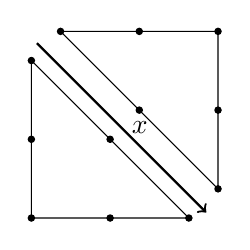
\begin{tikzpicture}[scale=2]
    \begin{scope}[xshift=-.1em,yshift=-.1em]
      \draw (0,0) -- (0,1) -- (1,0) -- (0,0);
      \draw[fill=black] (0,0) circle (0.02);
      \draw[fill=black] (0.5,0) circle (0.02);
      \draw[fill=black] (1,0) circle (0.02);
      \draw[fill=black] (0.5,0.5) circle (0.02);
      \draw[fill=black] (0,1) circle (0.02);
      \draw[fill=black] (0,0.5) circle (0.02);
    \end{scope}
    \draw[->,thick] (0,1.075) -- node[right]{$x$} (1.075,0);
    \begin{scope}[xshift=1.15cm,yshift=1.15cm,rotate=180]
      \draw (0,0) -- (0,1) -- (1,0) -- (0,0);
      \draw[fill=black] (0,0) circle (0.02);
      \draw[fill=black] (0.5,0) circle (0.02);
      \draw[fill=black] (1,0) circle (0.02);
      \draw[fill=black] (0.5,0.5) circle (0.02);
      \draw[fill=black] (0,1) circle (0.02);
      \draw[fill=black] (0,0.5) circle (0.02);
    \end{scope}
  \end{tikzpicture}
  \caption{Two adjacent triangles with support points}
  \label{fig:two-triangles-and-some-support-points}
\end{figure}

Since we are interested in the situation along the adjacent edges, which is a linear curve, we can remodel the problem to one dimension, which will reduce the computational complexity. This means that we do not actually construct two-variable polynomials for the whole triangles, but instead consider just polynomials that depend on one variable $x \in [0,1]$. The variable $x$ simultaneously traverses both adjacent edges.

\subsection{Constructing the polynomials}
\label{sec:constructing-polynomials}

As stated in the introduction, we have to construct $p^L$ and $p^R$, the polynomials describing the height and momentum of the right and left triangle respectively. We construct these polynomials by interpolating certain points.

We do so for the left and the right triangle, and for the height and the momentum. We call the points we've chosen the \emph{support points} for the left and right triangle. For convenience, we have decided to use a naming convention for these points. Assume that we have $n$ points for each triangle. Then we call the (components of the) points of the left triangle
\begin{equation*}
\left(x_1,\begin{pmatrix}
    h_1^R \\ u_1^R
  \end{pmatrix}\right), \dots , \left(x_n, \begin{pmatrix}
    h_n^R \\ u_n^R
  \end{pmatrix}\right)
\end{equation*}
and the points for the right triangle
\begin{equation*}
\left(x_1,\begin{pmatrix}
    h_1^L \\ u_1^L
  \end{pmatrix}\right), \dots , \left(x_n,\begin{pmatrix}
    h_n^L \\ u_n^L
  \end{pmatrix}\right),
\end{equation*}
i.e.\,we introduce a superscript indicating whether we are dealing with points within the left or the right triangle.

As you can see, each point consists of two components, first a position on the edge ($x_i, i \in \{1 \dots n\}$) and second a vector with the corresponding height and momentum, ($h_i^R$ and $u_i^R$ for the left triangle and $h_i^L$ and $u_i^L$ for the right, with $i \in \{1 \dots n\}$).

Intuitively one would think the support points should be equidistant to each other, but other distributions yield better results. Eventually we will need to integrate over the resulting function, which is numerically expensive. To compute it efficiently, we'll employ the Gaussian quadrature. This method requires its own support points to be applied, so we will choose our support points to coincide with them for easier computation. The corresponding results are summed up in section \ref{sec:results}.

However, we also investigated the situation for an equidistant distribution of support points. You find the corresponding results, as well as a short explanation of why this setting may be useful, in section \ref{sec:equidistant-distribution-of-support-points}.

To construct the polynomials assume we have a routine $interpolate\left(\{\left(x_i,y_i\right) \mid i \in \{1 \dots n\}\}\right)$. This routine takes a set of points $\left(x_1,y_1\right),\dots,\left(x_n,y_n\right)$ and returns the polynomial of degree $n-1$ that goes through all the points within the set (in practice this can be e.g. a Lagrange-Interpolation-Routine, Maple has a function \texttt{CurveFitting[PolynomialInterpolation]} ready for it). Here we introduce a notational shorthand for this cumbersome construct by simply writing $interpolate\left(x,y\right)$ for $interpolate\left(\{\left(x_i,y_i\right) \mid i \in \{1 \dots n\}\}\right)$.

We then generate four polynomials as follows:

\begin{itemize}
\item $p^L_h(x) := interpolate (x,h^L)$. Polynomial interpolating the height values for the left triangle.
\item $p^L_u(x) := interpolate (x,u^L)$. Polynomial interpolating the momentum values for the left triangle.
\item $p^R_h(x) := interpolate (x,h^R)$. Polynomial interpolating the height values for the right triangle.
\item $p^R_u(x) := interpolate (x,u^R)$. Polynomial interpolating the momentum values for the right triangle.
\end{itemize}

We then combine two polynomials into one to obtain the following:

\begin{equation*}
  p^L(x) :=
  \begin{pmatrix}
    p^L_h(x) \\ p^L_u(x)
  \end{pmatrix}, \quad
  p^R(x) :=
  \begin{pmatrix}
    p^R_h(x) \\ p^R_u(x)
  \end{pmatrix}
\end{equation*}

As was mentioned in section \ref{sec:flux-function-intro} $p^L$ and $p^R$ are actually functions that map $x \in [0,1]$ onto a vector containing the values of the height and the momentum polynomial for the respective triangle, we still call $p^L$ and $p^R$ polynomials to refer to the resulting functions, which we will be working with.

\subsection{What do we want to know?}
\label{sec:goal-intro}

What we eventually would like to do is to compare the following two things with each other:

\begin{description}
\item[Exact solution] We supply the polynomials $p^L$ and $p^R$ (depending on $x$) into the Lax-Friedrich-Flux, and compute its exact value. The resulting values are again polynomials depending on $x$. We call these polynomials $N\left(x\right)$ (a vector which has a polynomial for the height as its first component, while the second component represents the momentum).

\item[Approximate solution] We supply the support points into the Lax-Friedrich-Flux directly, and compute the resulting values, i.e.\,we compute the following for $i \in \{1 \dots n\}$:
  \begin{equation*}
    F_{LF}\left(
      \begin{pmatrix}
        h_i^R \\ u_i^R
      \end{pmatrix},
      \begin{pmatrix}
        h_i^L \\ u_i^L
      \end{pmatrix}
    \right) :=
    \begin{pmatrix}
      h_i^F \\ u_i^F
    \end{pmatrix} = F_i
  \end{equation*}

  We introduce shorthand notation $F_i$ for the resulting values. Each $F_i$ has the same structure as the $x_i$, only it's evaluated by the flux function. Next we interpolate the points (i.e.\,we interpolate the first components to obtain one polynomial, and we interpolate the second components to obtain another polynomial). The resulting polynomials are called $N^\prime\left(x\right)$ (interpreted like $N\left(x\right)$ as explained above).

  That is, we set
  \begin{equation*}
    N^\prime\left(x\right) :=
    \begin{pmatrix}
      interpolate\left(x,h^F\right) \\ interpolate\left(x,u^F\right)
    \end{pmatrix}
  \end{equation*}

\end{description}

Our goal will then be to compare $N\left(x\right)$ against $N^\prime\left(x\right)$ (component-wise, of course). We compare the quality of an approximation by considering the following term:

\begin{equation}
  \label{eq:integral-norm-definition}
  I := \int\limits_{x=0}^1 | N\left(x\right) - N^\prime\left(x\right) |\  dx,
\end{equation}
where the integration is to be understood component-wise.

\subsection{\texorpdfstring{How to evaluate $I$}{How to evaluate I}}
\label{sec:how-to-eval-I}

It is a nontrivial task to evaluate the integral in equation (\ref{eq:integral-norm-definition}). Even if we delegate most of the work to the symbolic math program \emph{Maple}, we experienced some pitfalls while evaluating the exact approach.

The main problem with exact integration is that Maple has to compute the zeroes of $N\left(x\right)-N^\prime\left(x\right)$, which is, depending on the degree of the polynomials, a time consuming task.

There are several possibilities to overcome this problem. The first that might come to one's mind is to use a Gaussian integration. However, using a Gaussian integration requires that the integrand at least ``looks somehow'' like a polynomial -- something we explicitly can \emph{not} be sure of.

So we had to use another approach. Here are the three we took into account:

\begin{itemize}
\item $N\left(x\right)$ and $N^\prime\left(x\right)$ intersect when supplied the support points, i.e.\,
  \begin{equation*}
    N\left(x_i^F\right) = N^\prime\left(x_i^F\right), \forall i \in \{1 \dots n\}.
  \end{equation*}

  Knowing this, we can derive some zeroes (but possibly not all). If we compute
  \begin{equation*}
    \sum\limits_{i=1}^{n-1} \left|\ \int\limits_{x=x_i}^{x_{i+1}} N\left(x\right) - N^\prime\left(x\right)\ dx \right|,
  \end{equation*}
  we get a more accurate result as an approximation for $I$ compared to simply computing the integral over $[0,1]$.

  If we moreover divide each interval $[x_i,x_{i+1}]$ into several smaller sub-intervals, and simply integrate over them, we can reduce the error ad libitum.

  While we can tweak this method by simply evaluating more and more sub-intervals, this comes at the price of more computations.
\item Another approach was to use Maple's numerical integration facilities. If we tell Maple to
  \begin{center}
    \texttt{evalf(Int(abs(N(x)-N(x)),x=0..1))},
  \end{center}
  we get a good result, if we wait long enough.

  We experimented with random polynomials and tried a few of them out, comparing the \texttt{evalf}-result to the exact integration. We experienced that the \texttt{evalf}-result was always equal to the actual result within an error of 0.001.

  However, this approach works only if \emph{all} variables are \emph{numbers}, i.e.\,if all points are instantiated to concrete values. If we want to plot a graph for a range of values for one or more of the points' components, at least one variable will not be a number, but will range within a certain interval. Thus, the \texttt{evalf}-approach has its drawbacks as well.
\item The last approach we tried was to divide the area under the function
  \begin{equation*}
    \left| N\left(x\right)-N^\prime\left(x\right) \right|
  \end{equation*}
  into several stripes, and compute the area of these stripes. The more stripes we have, the more accurate our result will be, at the expense of computation time.
\end{itemize}

We eventually went for the last of these approaches. It is just as well possible to use the second one, or the first, although this requires to tell Maple that it should \emph{first} make all necessary substitutions, and \emph{second} plot the resulting graphs. This is not only harder to accomplish but also results in a mess of code, but would not produce more accurate results, which is why we did not explore this option further.

You can find some more information about the developed tool in section \ref{sec:making-the-whole-thing-interactive}.

\subsection{Singularities}
\label{sec:singularities}

If we take a look at the second component of $I$, we can see that it contains a fraction (this is due to the flux function \ref{eqn:shallow-water-flux}, which contained a fraction itself). This means that there could be some singularities involved. If we integrate, we need to pay attention to these singularities, although we will see that they will have no practical relevance for us.

If we use two support points for each edge (all points except $p_1^L$ are $(10,0)$) and expand the term $N\left(x\right)-N^\prime\left(x\right)$, we can clearly see a fraction in its second component, i.e.\, the term describing the error in the momentum component. The fraction term in this example looks as follows (numerator omitted for simplicity):

\begin{equation*}
  \frac{1}{h_1\cdot(1.732 h_1 \cdot x - 17.320 x - 1.366 h_1 + 3.660)}
\end{equation*}

Remember from equation (\ref{eq:integral-norm-definition}) that the term $I$ integrates over $N\left(x\right)-N^\prime\left(x\right)$ from $x=0$ to $x=1$. Thus -- depending on the value of $h_1$ -- we run the risk that there is a singularity (w.r.t.\, the variable $x$). We can calculate that we have a singularity at
\begin{equation*}
  x_0=\frac{683\, h_1 - 1830}{866\, h_1 - 8600}.
\end{equation*}

Since we take the integral between 0 and 1, it is of particular interest if the value $x_0$ can be within the interval $\left[ 0,1 \right]$, since in this case we would integrate over a singularity where the integral is not (or at least might not be) properly defined. If it is a pole, which is likely in this situation, we would obtain extremely high values from the numerical integration over that domain.

We obtain that $x_0 \in \left[ 0,1 \right]$ only if $h_1 \leq 2.679$ or $h_1 \geq 37.322$. So we see that for this particular case we have singularities only for values of $h_1$ that differ greatly from all other values for the height (that are in this case set to 10).

We tried these calculations for other scenarios, including a variation in support points. The results were always the same, that the height would have to differ in absurd levels to even approach the required region of the singularity.

However, it is still important to note that these singularities do in fact occur. While they did not interfere with our calculations, similar application with largely differing sample values may encounter a problem at this point.

Analytically deriving a general formula for where these singularities occur is a difficult task due to the large number of variables. This is further complicated by the fact that the number of variables itself is not static but depends on the number of support points. We even encountered problems computing the exact $x$ values for the singularities for four support points, because of the complexity of the term, although they could still be found visually once the function was evaluated and plotted, coinciding with our previously computed results.

\newcommand{\fracsumme}{\mathtt{approx\_int}}

% It is convenient to research this fraction and look what happens if we set $h_1$ approximately to 1.6. Let us -- for simplicity -- assume that we numerically approximate this component of $I$ using five stripes (i.e. we take the function values at $x\in\left\{ 0, 0.25, 0.5, 0.75, 1 \right\}$). So, we can consider $\fracsumme(h_1,u_1) := \sum_{i=0}^4 \badfrac(\frac{i}{4})$ which is a part of what is plotted in figure \ref{fig:two-points-p1-wider-range}.

%If we evaluate this for corresponding values for $h_1$ and $u_1$ (i.e.\,in particular for $h_1\approx 1.6$ and $h_1\approx 0$), we obtain results summed up in table

% \begin{table}[ht]
%   \centering
%   \begin{tabular}[ht]{ll}
%     \hline
%     $\fracsumme(0,0)$ & -2.6 \\
%     $\fracsumme(0,1)$ & -11.3 \\
%     $\fracsumme(0,0)$ & -27.0 \\
%     $\fracsumme(0,0)$ & -49.7 \\
%     $\fracsumme(1.6,0)$ & -0.87 \\
%     $\fracsumme(1.6,1)$ & -2.52 \\
%     $\fracsumme(1.6,2)$ & -13.9 \\
%     $\fracsumme(1.6,3)$ & -34.9 \\
%   \end{tabular}
%   \caption{Selected values for the term $\fracsumme$ depending upon $h_1$ and $u_1$}
%   \label{tab:selected-values-for-fracsumme}
% \end{table}

\section{\texorpdfstring{Visualizing the error term $I$}{Visualizing the error term I}}
\label{sec:making-the-whole-thing-interactive}

We are now going to plot (the two components of) the term $I$ as described in equation (\ref{eq:integral-norm-definition}). First, we have to elaborate on some necessary considerations when it comes plotting such a complicated term. Afterwards, we present our tool that was developed to simplify plotting as much as possible.

\subsection{A word on visualization}
\label{sec:a-word-on-visualization}

Before we actually go into visualizing the error term, let us introduce some concepts that will be useful later when it comes to plotting.

Consider some well-known plots known from school, e.g. the graphs for the functions $y=2\cdot x+3$ or $y=x^2$. These plots are probably well-known to every reader of this paper -- simply a horizontal $x$-axis, and a vertical $y$-axis.

\subsubsection{Functions with parameters}

Let us now consider a slightly more complicated function, namely

\begin{equation*}
  y = a\cdot x+1.
\end{equation*}

This equation describes a line going through point $(0,1)$ with varying gradient, namely $a$. That is, we actually have a whole collection of lines given by this equation. If one wants to plot ``the function'' $y=a\cdot x + 1$, one has in principle two possibilities:

\begin{itemize}
\item Focus on specific values of $a$ and plot $y=a\cdot x + 1$ for these values of $a$.
\item Generate a 3d-plot for varying values of $a$ and $x$. This plot has then two axes for $a$ and $x$ spanning two dimensions, the resulting value $y$ is then denoted by the last dimension.

  That is, each point contained in the graph of this 3d-plot has three coordinates $(x,a,y)$, and these three coordinates have to suffice the condition $y=a\cdot x + 1$.
\end{itemize}

You can compare the two methods in figure \ref{fig:simple-parametric-functions}. Note that you can interpret the lines in the two dimensional plot as ``slices'' from the three dimensional plot.

\begin{figure}[ht]
  \centering
  \subfigure[Choosing particular values for $a$]{
    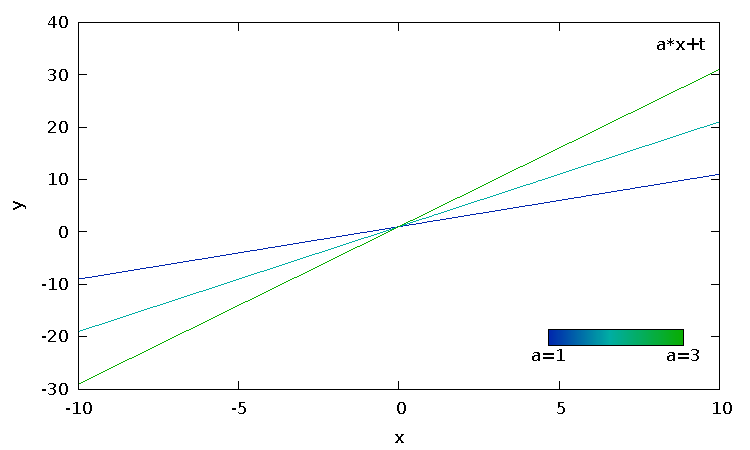
\includegraphics[scale=0.5]{simple_parametric_2d.pdf}
  }
  \subfigure[A three dimensional plot]{
    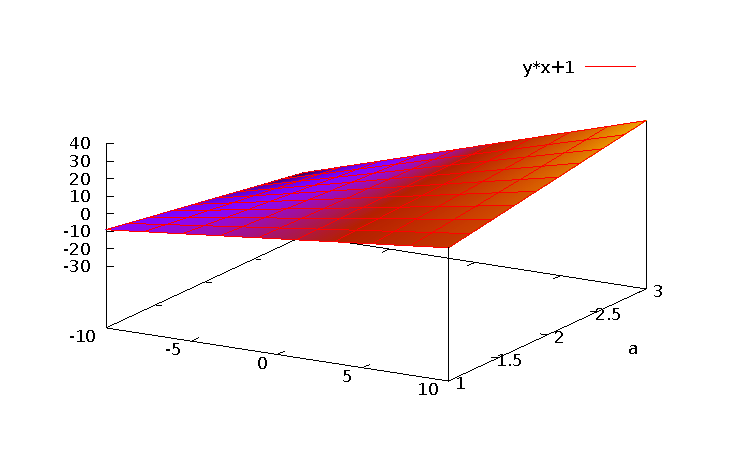
\includegraphics[scale=0.5]{simple_parametric_3d.pdf}
  }
  \caption{Plotting simple parametric functions using different approaches}
  \label{fig:simple-parametric-functions}
\end{figure}

Now, let us extend the above function by another variable and consider the function

\begin{equation*}
  y = a\cdot x+b.
\end{equation*}

As you can see, this function contains two parameters, namely $a$ and $b$. Again, if we want to plot this (collection of) line(s), we have several possibilities:

\begin{itemize}
\item Focus on specific values for $a$ and $b$ and generate a plot for the combinations of $a$ and $b$ under considerations.
\item Focus on specific values for $a$, and draw a 3d-plot (for each value of $a$ under consideration) having two axes that then describe $x$ and $a$, while $y$ is then represented by the remaining dimension.
\item Similar to the previous possibility, one could focus on $b$ (instead of $a$) and draw 3d-plots having two axes that then describe $x$ and $b$, while $y$ is then represented by the remaining dimension.
\end{itemize}

Of course, as the number of parameters increases, the number of possibilities for plotting grows drastically. This is why we have to pick specific assignments for parameters and generate the corresponding plots.

\subsection{Some considerations to take into account}
\label{sec:some-considerations}

Recall from section \ref{sec:constructing-polynomials}, that the terms $p^L$ and $p^R$ depend on the chosen support points. Moreover, $N\left(x\right)$ depends on these polynomials. Thus, the term $N\left(x\right)-N^\prime\left(x\right)$ also depends on the polynomials and by extension on the support points. This means, we have $4n$ variables\footnote{We have $n$ points for each of the two adjacent edges, each point consisting of a height and a momentum component, resulting in $4n$ variables.} in this term.
This implies that $I$ (see equation (\ref{eq:integral-norm-definition})) also depends on the single points $
\begin{pmatrix}
  h_1^L \\ u_1^L
\end{pmatrix},\dots,
\begin{pmatrix}
  h_n^L \\ u_n^L
\end{pmatrix},
\begin{pmatrix}
  h_1^R \\ u_1^R
\end{pmatrix},\dots,
\begin{pmatrix}
  h_n^R \\ u_n^R
\end{pmatrix}$. When it comes to plotting, the amount of variables requires us to later mask out some of them to be able to obtain useful plots.

We could interpret $I$ as a function over these $4n$ values onto a two-component vector containing the integral from the $h$ and $u$ components. If we were precise, we would then write it in function notation $
I\left(\begin{pmatrix}
    h_1^L \\ u_1^L
  \end{pmatrix},\dots,
  \begin{pmatrix}
    h_n^L \\ u_n^L
  \end{pmatrix},
  \begin{pmatrix}
    h_1^R \\ u_1^R
  \end{pmatrix},\dots,
  \begin{pmatrix}
    h_n^R \\ u_n^R
  \end{pmatrix}\right)$ instead of simply $I$. However, most of the time we prefer $I$, since we are interested in notational simplicity.

We decided to use 3D plots, where we have two axes representing two of the $4n$ variables. All the other variables are fixed to certain values.
% Later we will explain how we can visualize $I$. Since there are many variables to choose, we decided to fix all but one point and visualize the result.
For example, if we fixed all points to $
\begin{pmatrix}
  10 \\ 0
\end{pmatrix}
$ except the first point, this would mean we are interested in
\begin{equation*}
  I\left(
    \begin{pmatrix}
      h_1^L \\ u_1^L
    \end{pmatrix},
    \begin{pmatrix}
      10 \\ 0
    \end{pmatrix}, \dots,
    \begin{pmatrix}
      10 \\ 0
    \end{pmatrix}
  \right).
\end{equation*}

We can now use a 3D plot with the $x$ axis representing $h_1^L$ and the $y$ axis representing $u_1^L$. The $z$ value would then represent the resulting value of $I$.

\subsection{Plotting tool}
\label{sec:plotting-tool-intro}

To plot our results we considered several options. Maple supports dynamic plotting to a certain degree, and since we used it for some of our previous symbolic and numeric computation, we tried employing it to obtain the plots we need. Essentially, one can obtain a window with movable sliders that change a plot adjusting to it.

However, we realized that this method had some downsides. We always are interested in plotting two graphs, one for the height error and one for the momentum error (both components of $I$). Showing two plots simultaneously affected by the same sliders proved to be a challenge, and was not doable with the native plotting services due to limited customization. It may have been able to write a custom Maplet (interactive Maple applet) which did what we wanted, but that turned out to be just as cumbersome due to Maple's limited applet functionality.

Moreover, we wanted to be able to quickly switch the coordinate axes, so that we can compare plots with each other in real time, which also did not work with the native implementation. Finally, Maple's user interface is not intended to be used with that many variables, which posed a challenge for our $4n$ variables in $I$. The only alternative would have been to cut some of them out, which would make the tool less interactive.

So we decided to develop a tool that helps us visualizing our data properly. We implemented a simple program that is capable of doing the following:

\begin{itemize}
\item Read two functions from a file. In our case these functions will be the components of $I$, which are the contents of $N\left(x\right)-N^\prime\left(x\right)$ (i.e.\,the integrand within the integral of $I$). This file is generated by Maple in our case, since we use it for most of our computations, but it can be created manually by the user as well.
\item Extract variable names from the mathematical expressions extracted from the file (in our case, this will be mainly the variables $u_i$ and $h_i$ in a suitable string representation\footnote{We decided to use a simple scheme for the internal variable names: $u_1^L$ becomes \texttt{u\_1} and $u_1^R$ becomes \texttt{U\_1}, while $h_3^L$ becomes \texttt{h\_3} and $h_4^R$ becomes \texttt{H\_4}.}). The variable $x$ is handled separately since this is the variable that we want to integrate over to compute $I$.
\item Offer a way to dynamically change the values of the variables (i.e. the $u_i$ and $h_i$). This is achieved by a slider for each variable (see figure \ref{subfig:plotting-tool-variables}).
\item Numerically evaluate $I$ for the given functions. This is achieved using the technique described in section \ref{sec:how-to-eval-I}.
\item Choose any of the variables to be used as $x$ and $y$ coordinates for a 2D or 3D plot.
\item Plot $I$ using \texttt{gnuplot}.
\item Export plots and generate a proper TeX-file.
\end{itemize}

The implementation turned out to be quite useful and easier to handle than any equivalent Maple solutions. Figure \ref{fig:plotting-tool} shows what the tool looks like.

\begin{figure}[ht]
  \centering
  \subfigure[Adjusting variables and axes]{
    \label{subfig:plotting-tool-variables}
    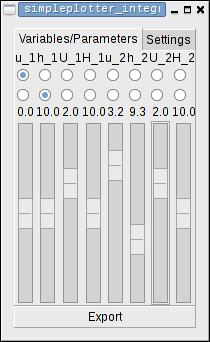
\includegraphics[scale=0.5]{simpleplotter_screen1.png}
  }
  \subfigure[Gnuplot settings/Settings for numerical integration]{
    \label{subfig:plotting-tool-gnuplot}
    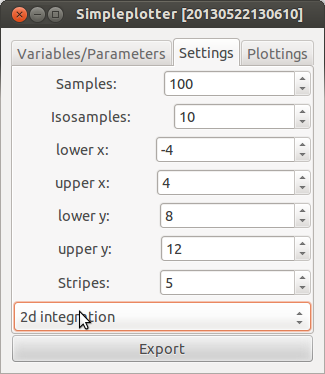
\includegraphics[scale=0.5]{simpleplotter_screen2.png}
  }
  \caption{Plotting tool window.}
  \label{fig:plotting-tool}
\end{figure}

Subfigure \ref{subfig:plotting-tool-variables} shows the page that is used to adjust the variables. As you can see, the tool has detected variables \texttt{u\_1}, \texttt{h\_1}, \texttt{U\_1}, and so on. Moreover you can see that e.g.\, the parameter \texttt{u\_2} is set to a value of 3.2, while \texttt{u\_1} is set to 0.0.

The radio buttons determine which variables are used as axes. In subfigure \ref{subfig:plotting-tool-variables}, in the first option row, the column for \texttt{u\_1} is selected, while in the second row, we chose \texttt{h\_1}. This means that the plotter uses \texttt{u\_1} as $x$ axis, and \texttt{h\_1} as $y$ axis for the 3D plot.

Subfigure \ref{subfig:plotting-tool-gnuplot} shows exemplary settings for plotting. ``Samples'' and ``Isosamples'' are gnuplot-specific parameters that determine how fine-grained gnuplot is plotting the curve. A hundred samples and ten isosamples have shown to be a fitting balance between an accurate graph and an acceptable computation time. The settings for lower and upper $x$ and $y$ values determine the range that is plotted by gnuplot.

The parameter ``stripes'' determines how many stripes are used to numerically evaluate the integral $I$. After trying some values we found out that using less than five stripes is noticeably inaccurate. However, using more than five stripes does not significantly affect the result.

\subsection{How to interpret the graphs}
\label{sec:how-to-interpret-graphs}

All the plots in this document are generated using our tool. We said that our tool reads two functions from a file and interprets them as the two components of $N\left(x\right)-N^\prime\left(x\right)$. The tool generates two plots that are labeled ``0. Function'' and ``1. Function''. In our case ``0. Function'' represents the error in the $h$ component (height), while ``1. Function'' stands for the error in the $u$ component (momentum).

To understand how our plots work, we can take a look at figure \ref{fig:two-points-all-the-same}. In this example, we used 2 points on each triangle and edge. That is, we have four (relevant) points in total, \emph{two of which} we have plotted here. This is why figure \ref{fig:two-points-all-the-same} has \emph{two} sub-figures.

Looking at sub-figure \ref{subfig:two-points-p1-height-momentum}, its caption says that point $p_1^L$ is varying. To be precise, its height and momentum vary along the plot axes.

The first part of this caption tells us that we are fixing \emph{all points except} $p_1^L$ to a specific value (in this case it was $
\begin{pmatrix}
  10 \\ 0
\end{pmatrix}
$), i.e.\,we are considering the term $I\left(
  \begin{pmatrix}
    10 \\ 0
  \end{pmatrix},
  \begin{pmatrix}
    h_2^R \\ u_2^R
  \end{pmatrix},
  \begin{pmatrix}
    10 \\ 0
  \end{pmatrix},
  \begin{pmatrix}
    10 \\ 0
  \end{pmatrix}
\right)$.

% In subfigure \ref{subfig:fixing-p2-in-first-example}, we deal with a function that has two variables (namely $h_2^R$ and $u_2^R$). Thus, we can create a 3D plot showing this function. Please remember that $I$ was a \emph{vector} containing two components. This is why subfigure \ref{subfig:fixing-p2-in-first-example} contains two plots. The left plot stands for the $h$ component, while the right one represents the $u$ component.

The orientation of the axes is displayed in figure \ref{fig:orientation-of-axes}.

\begin{figure}[th]
  \centering
  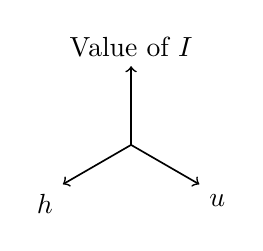
\begin{tikzpicture}
    \draw[->,semithick] (0,0) -- (0,1) node[above]{Value of $I$}; % z
    \draw[->,semithick] (0,0) -- +(-30:1) node[below right]{$u$}; % x
    \draw[->,semithick] (0,0) -- +(210:1) node[below left]{$h$}; % y
  \end{tikzpicture}
  \caption{Orientation of the axes used for our 3D plots}
  \label{fig:orientation-of-axes}
\end{figure}

To plot $u$ and $h$ we need to know their respective ranges as well. This is noted in the caption of the whole figure. For example, in figure \ref{fig:two-points-all-the-same}, the values for $u$ are in $[8, 12]$ and the values for $h$ in $[-4,4]$.

% Looking back at the caption of the subfigure, which had ``1/0.04'' in the latter part (subfigure \ref{subfig:fixing-p2-in-first-example}). This tells us the range of the values of $I$ (i.e.\,the ``$z$ axis''). To be precise, the firs part tells us that the maximal plotted value for the h component is 1, while the maximal $u$ component value is 0.04. A single number indicates a range between 0 and that number, while an explicit range indicates the given range (for an example, see \ref{subfig:example-with-range}, where the $h$ component plot range goes from 0.25 to 0.55, and the $u$ component from 0 to 0.03).

\section{Results: Distribution of support points according to Gaussian quadrature}
\label{sec:results}

We implemented several scenarios and present the outcome of some of them using the support points one would use when doing a Gaussian quadrature. The $x$ values of these support points are summed up in table \ref{tab:x-coordinates-gauss-quadrature} and can be read in any book on Gaussian quadrature.

\begin{table}[ht]
  \renewcommand\arraystretch{1.5}
  \centering
  \begin{tabular}[ht]{cl}
    Order & $x$-coordinates \\
    \hline
    2 & $\frac{1}{2}-\frac{1}{6}\cdot \sqrt{3},\  \frac{1}{2}+\frac{1}{6}\cdot \sqrt{3}$ \\
    3 & $-\frac{1}{10}\cdot \sqrt{15}+\frac{1}{2} ,\  0.5,\  \frac{1}{10}\cdot \sqrt{15}+\frac{1}{2}$ \\
    \hline
  \end{tabular}
  \caption{$x$-coordinates of support points for Gauss-Quadrature}
  \label{tab:x-coordinates-gauss-quadrature}
\end{table}

\subsection{Setting all support points to the same value}
\label{sec:setting-all-support-points-to-the-same-value}

First we set all support points to one single value ensuring homogenous height and momentum. Then, we tackle each point individually and let their values range over a certain domain.

% 8 variables in here:
% u_1 = 0.0, h_1 = 10.0, U_1 = 0.0, H_1 = 10.0, u_2 = 0.0, h_2 = 10.0, U_2 = 0.0, H_2 = 10.0
%\renewcommand{\zoomfactor}{1.2}

\begin{figure}[ht]
  \centering
  \subfigure[Impulse error for varying point $p_1$] {
    \label{subfig:two-points-p1-height-momentum}
    % \includegraphics[scale=\zoomfactor]{{{2_punkte_alles_10_0/x_y_0.0_10.0_0.0_10.0_0.0_10.0f0}}}
    % \begin{tikzpicture}
    %   \node at (0,0) {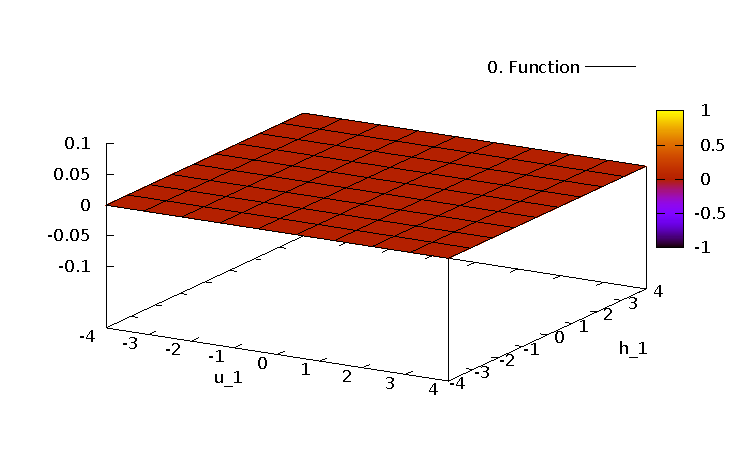
\includegraphics[scale=\zoomfactor]{zero_plots/u1h1}};
    %   \fill[white] (.8,1.2) rectangle (1.75,1.5);
    %   \node[align=right, text width=3cm] at (.2, 1.33) {\textsf{\tiny{Height error}}};
    % \end{tikzpicture}
    \begin{tikzpicture}
      \node at (0,0) {\includegraphics[scale=\zoomfactor]{{{2_punkte_alles_10_0/x_y_0.0_10.0_0.0_10.0_0.0_10.0f1}}}};
      \fill[white] (.8,1.2) rectangle (1.75,1.5);
      \node[align=right, text width=3cm] at (.2,1.33) {\textsf{\tiny{Impulse error}}};
    \end{tikzpicture}
  }
  \subfigure[Impulse error for varying point $p_2$] {
    \label{subfig:fixing-p2-in-first-example}
    % 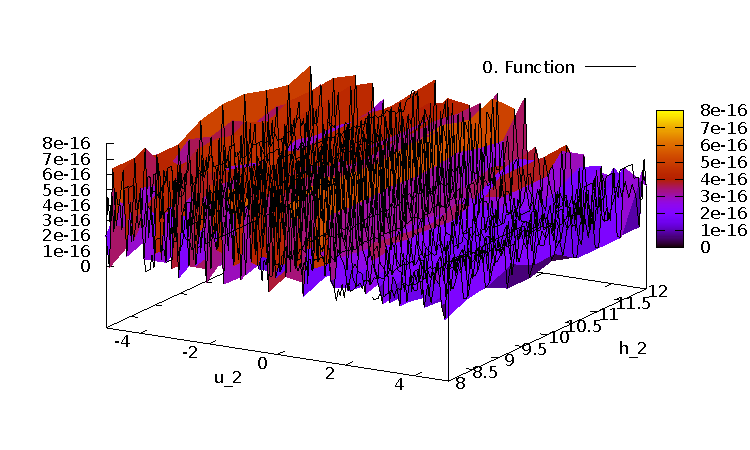
\includegraphics[scale=\zoomfactor]{{{2_punkte_alles_10_0/0.0_10.0_0.0_10.0_x_y_0.0_10.0f0}}}
    % \begin{tikzpicture}
    %   \node at (0,0) {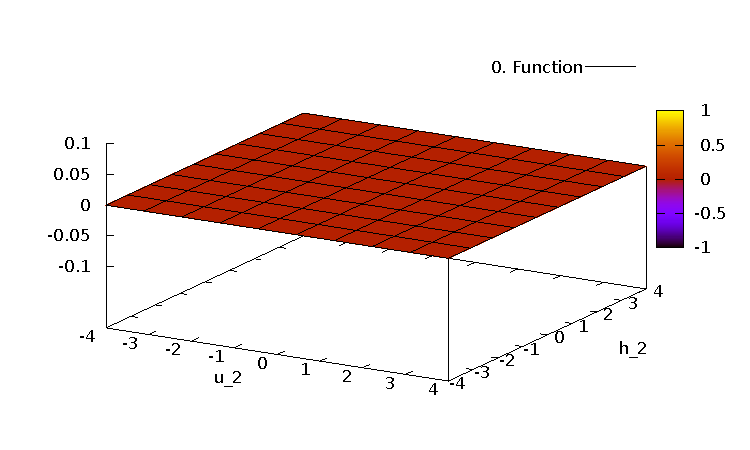
\includegraphics[scale=\zoomfactor]{zero_plots/u2h2}};
    %   \fill[white] (.8,1.2) rectangle (1.75,1.5);
    %   \node[align=right, text width=3cm] at (.2,1.33) {\textsf{\tiny{Height error}}};
    % \end{tikzpicture}
    \begin{tikzpicture}
      \node at (0,0) {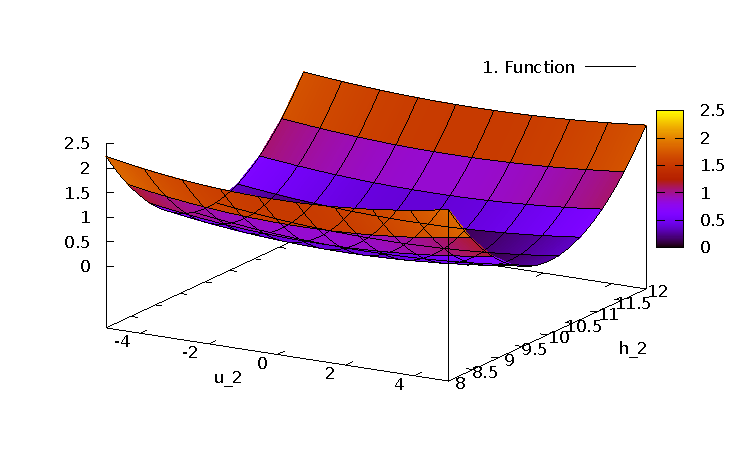
\includegraphics[scale=\zoomfactor]{{{2_punkte_alles_10_0/0.0_10.0_0.0_10.0_x_y_0.0_10.0f1}}}};
      \fill[white] (.8,1.2) rectangle (1.75,1.5);
      \node[align=right, text width=3cm] at (.2,1.33) {\textsf{\tiny{Impulse error}}};
    \end{tikzpicture}
  }
  \caption{Two points for each triangle. All support points have height 10 and impulse 0. $h$ ranges from 8 to 12, $u$ from -4 to 4. Note that the behaviour is completely symmetric. Varying the points of the other triangle (i.e. $p_1^R$ resp. $p_2^R$ yields the same plots.}
  \label{fig:two-points-all-the-same}
\end{figure}

%%% Local Variables:
%%% TeX-master: "../results.tex"
%%% End:

%%% Local Variables:
%%% TeX-master: "../results.tex"
%%% End:


Figure \ref{fig:two-points-all-the-same} shows the case for two points on each adjacent edge. Each subfigure shows what happens if we fix all but one specific support point. For example, subfigure \ref{subfig:fixing-p2-in-first-example} shows what happens if we fix all support points except $p_2^L$ (containing the variables $h_2^L$ and $u_2^L$) and let $h_2^L$ range from 8 to 12 and $u_2^L$ from $-4$ to 4. The left part of subfigure \ref{subfig:fixing-p2-in-first-example} shows the (normalized) error in the $h$ component, while the right half depicts the error in the $u$ component. As can be seen, the error in the $h$ component is always zero in the range depicted here (about $10^{-15}$ to be precise, which can be interpreted as numerical error). We will generally omit plots that show no error like that.

As the plot shows, the error for the $h$ component ranges up to 2.5.

We did the same thing for three support points along each edge (and it can be done for an arbitrary number of support points). You can see the results in figure \ref{fig:three-points-equal}. In general it seems that the structure of the error plots is quite similar across different settings: the error in the height component is almost zero, while the error in the momentum component looks similar to the ones seen in figure \ref{fig:two-points-all-the-same}.

% 12 variables in here:
% u_1 = 0.0, h_1 = 10.0, U_1 = 0.0, H_1 = 10.0, u_2 = 0.0, h_2 = 10.0, U_2 = 0.0, H_2 = 10.0, u_3 = 0.0, h_3 = 10.0, U_3 = 0.0, H_3 = 10.0
\begin{figure}[ht]
\centering
  \subfigure[Height and impulse for point $p_1^L$ resp. $p_1^R$] {
    \begin{tikzpicture}
      \node at (0,0) {\includegraphics[scale=\zoomfactor]{{{3_punkte_gleich/x_y_0.0_10.0_0.0_10.0_0.0_10.0_0.0_10.0_0.0_10.0f0}}}   };
      \fill[white] (.8,1.2) rectangle (1.75,1.5);
      \node[align=right, text width=3cm] at (.2,1.33) {\textsf{\tiny{Height error}}};
    \end{tikzpicture}
    \begin{tikzpicture}
      \node at (0,0) {\includegraphics[scale=\zoomfactor]{{{3_punkte_gleich/x_y_0.0_10.0_0.0_10.0_0.0_10.0_0.0_10.0_0.0_10.0f1}}}   };
      \fill[white] (.8,1.2) rectangle (1.75,1.5);
      \node[align=right, text width=3cm] at (.2,1.33) {\textsf{\tiny{Impulse error}}};
    \end{tikzpicture}
  }

  \subfigure[Height and impulse for point $p_2^L$ resp. $p_2^R$] {
    \begin{tikzpicture}
      \node at (0,0) {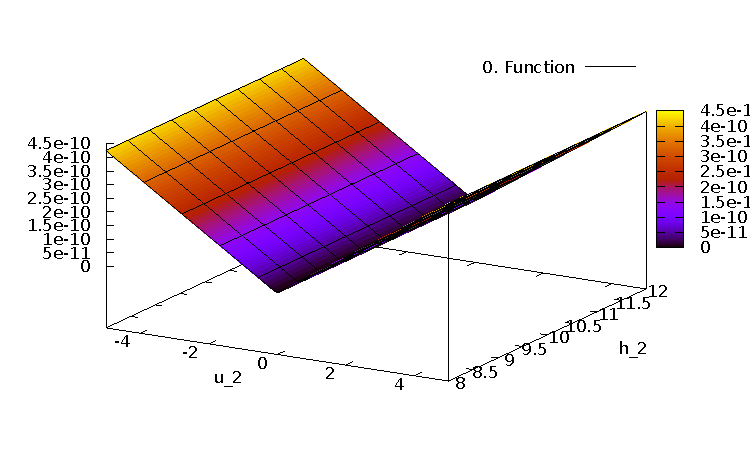
\includegraphics[scale=\zoomfactor]{{{3_punkte_gleich/0.0_10.0_0.0_10.0_x_y_0.0_10.0_0.0_10.0_0.0_10.0f0}}}   };
      \fill[white] (.8,1.2) rectangle (1.75,1.5);
      \node[align=right, text width=3cm] at (.2,1.33) {\textsf{\tiny{Height error}}};
    \end{tikzpicture}
    \begin{tikzpicture}
      \node at (0,0) {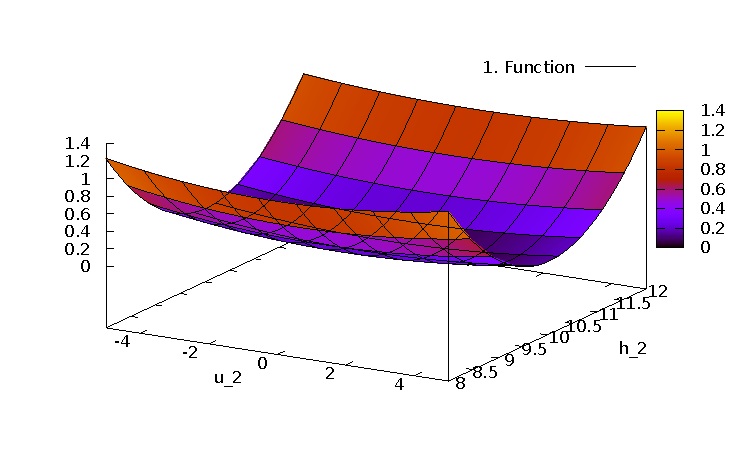
\includegraphics[scale=\zoomfactor]{{{3_punkte_gleich/0.0_10.0_0.0_10.0_x_y_0.0_10.0_0.0_10.0_0.0_10.0f1}}}   };
      \fill[white] (.8,1.2) rectangle (1.75,1.5);
      \node[align=right, text width=3cm] at (.2,1.33) {\textsf{\tiny{Impulse error}}};
    \end{tikzpicture}
  }

  \subfigure[Height and impulse for point $p_3^L$ resp. $p_3^R$] {    
    {    
      \begin{tikzpicture}
        \node at (0,0) {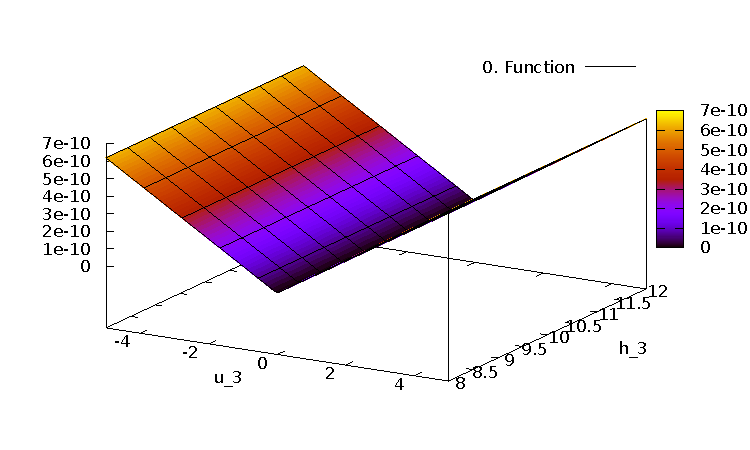
\includegraphics[scale=\zoomfactor]{{{3_punkte_gleich/0.0_10.0_0.0_10.0_0.0_10.0_0.0_10.0_x_y_0.0_10.0f0}}}   };
        \fill[white] (.8,1.2) rectangle (1.75,1.5);
        \node[align=right, text width=3cm] at (.2,1.33) {\textsf{\tiny{Height error}}};
      \end{tikzpicture}
    }
    {    
      \begin{tikzpicture}
        \node at (0,0) {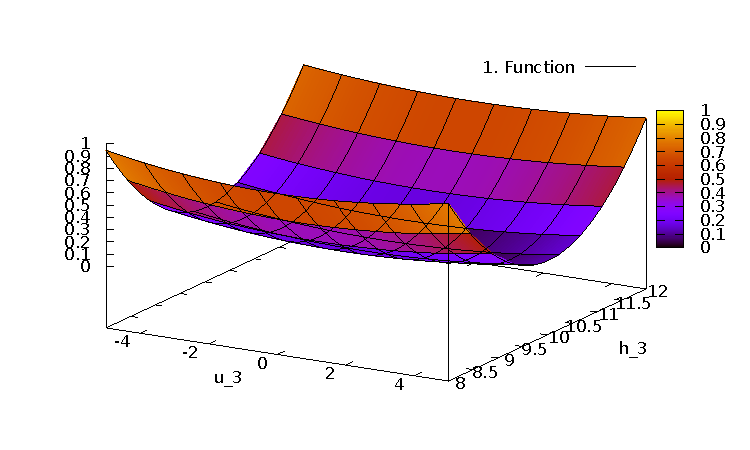
\includegraphics[scale=\zoomfactor]{{{3_punkte_gleich/0.0_10.0_0.0_10.0_0.0_10.0_0.0_10.0_x_y_0.0_10.0f1}}}   };
        \fill[white] (.8,1.2) rectangle (1.75,1.5);
        \node[align=right, text width=3cm] at (.2,1.33) {\textsf{\tiny{Impulse error}}};
      \end{tikzpicture}
    }
  }

    % 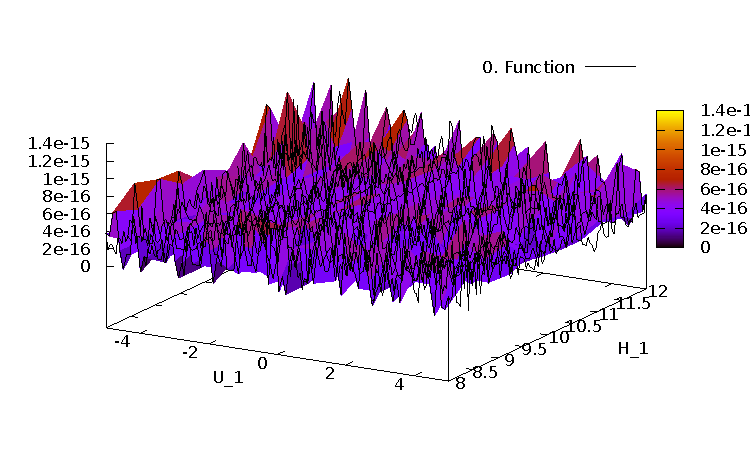
\includegraphics[scale=\zoomfactor]{{{3_punkte_gleich/0.0_10.0_x_y_0.0_10.0_0.0_10.0_0.0_10.0_0.0_10.0f0}}}   
    % 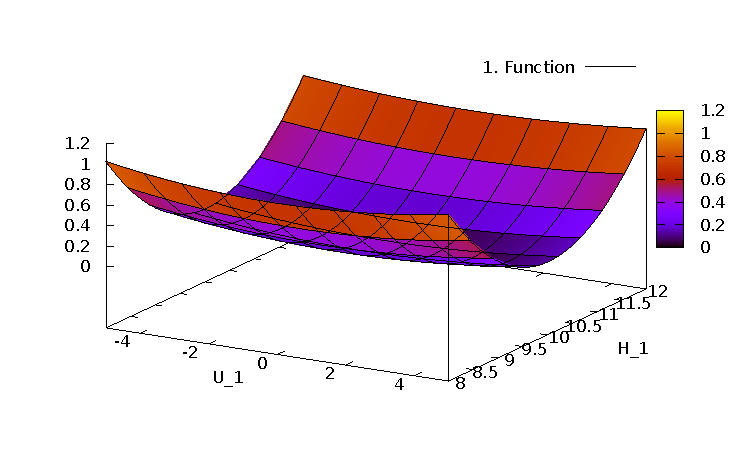
\includegraphics[scale=\zoomfactor]{{{3_punkte_gleich/0.0_10.0_x_y_0.0_10.0_0.0_10.0_0.0_10.0_0.0_10.0f1}}}   
  % \subfigure[] {    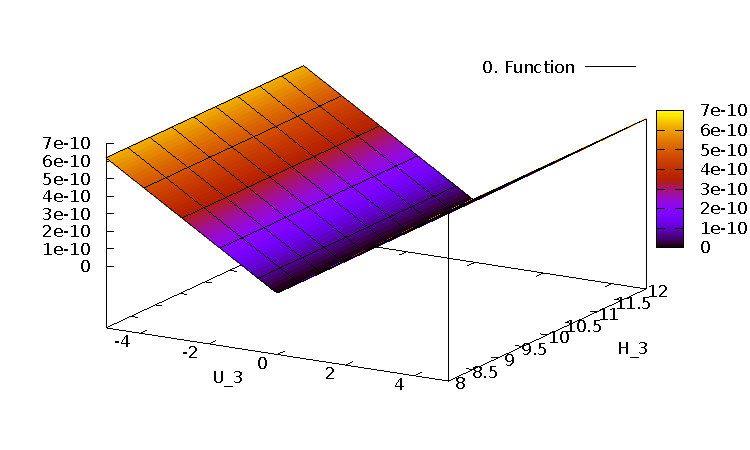
\includegraphics[scale=\zoomfactor]{{{3_punkte_gleich/0.0_10.0_0.0_10.0_0.0_10.0_0.0_10.0_0.0_10.0_x_yf0}}}   }
  % \subfigure[] {    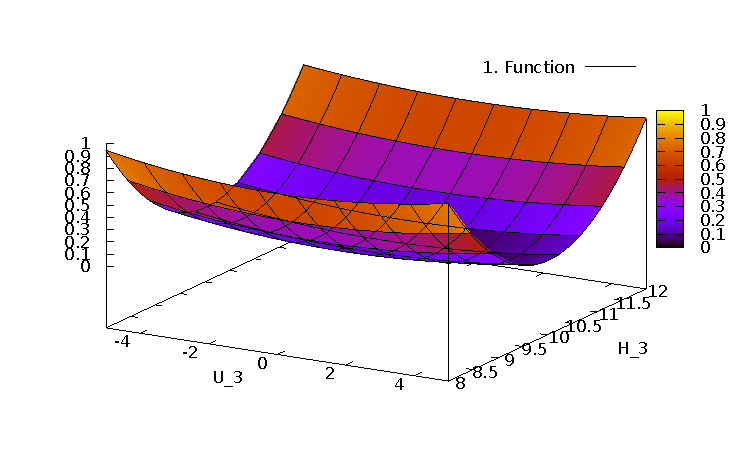
\includegraphics[scale=\zoomfactor]{{{3_punkte_gleich/0.0_10.0_0.0_10.0_0.0_10.0_0.0_10.0_0.0_10.0_x_yf1}}}   }

  % \subfigure[] {    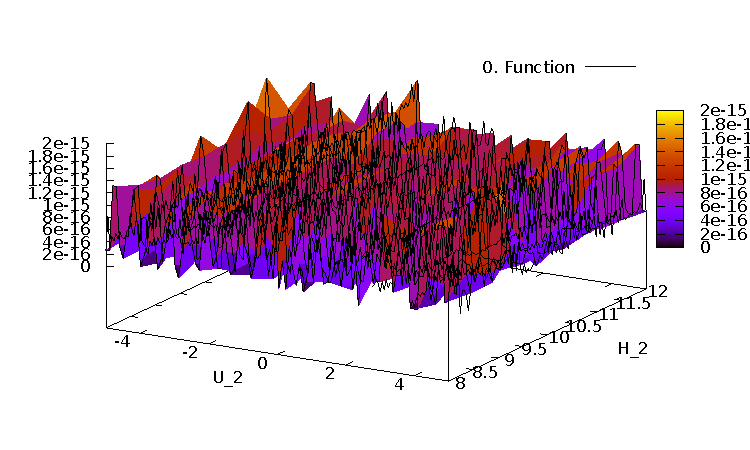
\includegraphics[scale=\zoomfactor]{{{3_punkte_gleich/0.0_10.0_0.0_10.0_0.0_10.0_x_y_0.0_10.0_0.0_10.0f0}}}   }
  % \subfigure[] {    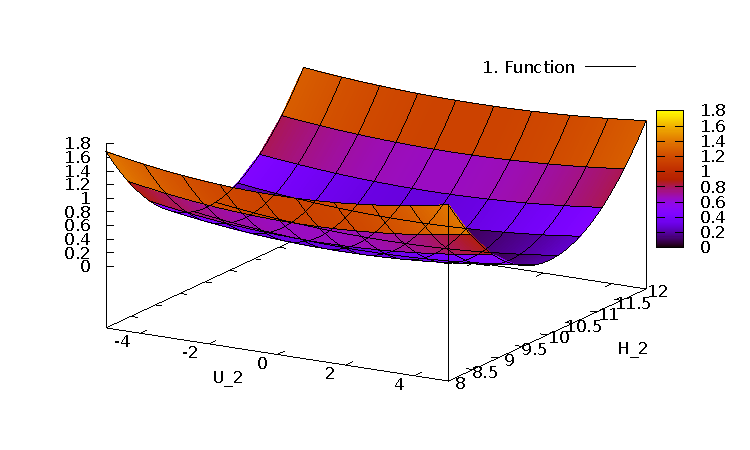
\includegraphics[scale=\zoomfactor]{{{3_punkte_gleich/0.0_10.0_0.0_10.0_0.0_10.0_x_y_0.0_10.0_0.0_10.0f1}}}   }
  \caption{Three points for each triangle. All points have height 10, impulse 0. The remaining points ($P_1, P_2$ and $P_3$) are not plotted since their plots look exactly the same.}
  \label{fig:three-points-equal}
\end{figure}

%%% Local Variables:
%%% TeX-master: "../results.tex"
%%% End:

%%% Local Variables:
%%% TeX-master: "../results.tex"
%%% End:


\subsection{Singularities}
\label{sec:plots-discontinuities}

When we look at figure \ref{subfig:fixing-p2-in-first-example}, we see that the error in the momentum component looks somewhat like a parabola with respect to the variable $h_1$. We see a smooth curve.

Remember that we saw in section \ref{sec:singularities} that there might be singularities. We will now see a plot that exposes these singularities to us.

% 8 variables in here:
% u_1 = 0.0, h_1 = 10.0, U_1 = 0.0, H_1 = 10.0, u_2 = 0.0, h_2 = 10.0, U_2 = 0.0, H_2 = 10.0
\begin{figure}[h!t]
  \centering
  % \subfigure[Height error] {
  % \includegraphics[scale=\zoomfactor]{{{2_points_def_luecke/x_y_0.0_10.0_0.0_10.0_0.0_10.0f0}}}
  % }
  %   \subfigure[Momentum error] {
  \begin{tikzpicture}
    \node at (0,0) {\includegraphics[scale=\zoomfactor]{{{2_points_def_luecke/x_y_0.0_10.0_0.0_10.0_0.0_10.0f1}}}};
    \fill[white] (.8,1.2) rectangle (1.75,1.5);
    \node[align=right, text width=3cm] at (.2,1.33) {\textsf{\tiny{Momentum error}}};
  \end{tikzpicture}
  % }
  \caption{Plotting the momentum error depending on $p_1$ for a wider range. All other points are $(10,0)$.}
  \label{fig:two-points-p1-wider-range}
\end{figure}

%%% Local Variables:
%%% TeX-master: "../results.tex"
%%% End:

%%% Local Variables:
%%% TeX-master: "../results.tex"
%%% End:


Figure \ref{fig:two-points-p1-wider-range} shows a plot that was created using two points per edge, each point having coordinates $(10,0)$. We use the coordinates of $p_1^L$ as axes (i.e.\,$h_1$ and $u_1$). But this plot's axes now have a wider range than the ones in previous plots. As you can see there, the error suddendly grows to about 200 -- a much larger value t han the one we have seen before! We realize that these discontinuities arise if $h_1$ takes a values of about 1.6 and 0. In fact, there are even more discontinuities that can not be seen here since they occur at more distant values for $h_1$.

\subsection{One point variation}
\label{sec:one-point-variation}

Up until now, we saw what the plots look like if all points have the same value. We are now goint to inspect what happens if the single points have different values.

\subsubsection{\texorpdfstring{Decreasing the height of $p_1^L$}{Decreasing the height of p1L}}
\label{sec:decreasing-height-p1}

Now we alter the previously described experiment in one detail. We fix all points as before, but we alter one single point slightly. We do this in order to find out if specific points might have more impact than others.

We start off by using three points per edge, setting each point to $
\begin{pmatrix}
  10 \\ 0
\end{pmatrix}$ except $p_1^L$ which is set to $
\begin{pmatrix}
  9 \\ 0
\end{pmatrix}
$ (i.e.\,we decrease the height component of $p_1^L$).

% 12 variables in here:
% u_1 = 0.0, h_1 = 9.0, U_1 = 0.0, H_1 = 10.0, u_2 = 0.0, h_2 = 10.0, U_2 = 0.0, H_2 = 10.0, u_3 = 0.0, h_3 = 10.0, U_3 = 0.0, H_3 = 10.0
\begin{figure}[h!t]
\centering
% \subfigure[] { \includegraphics[scale=\zoomfactor]{{{3_punkte_1_geschwindigkeit_verringert/x_y_0.0_10.0_0.0_10.0_0.0_10.0_0.0_10.0_0.0_10.0f0}}} }
% \subfigure[] { \includegraphics[scale=\zoomfactor]{{{3_punkte_1_geschwindigkeit_verringert/x_y_0.0_10.0_0.0_10.0_0.0_10.0_0.0_10.0_0.0_10.0f1}}} }

% \subfigure[Height for point $p_2^L$] {
%   \label{subfig:height-p1-three-points-height-verringert}
%   \begin{tikzpicture}
%     \node at (0,0) {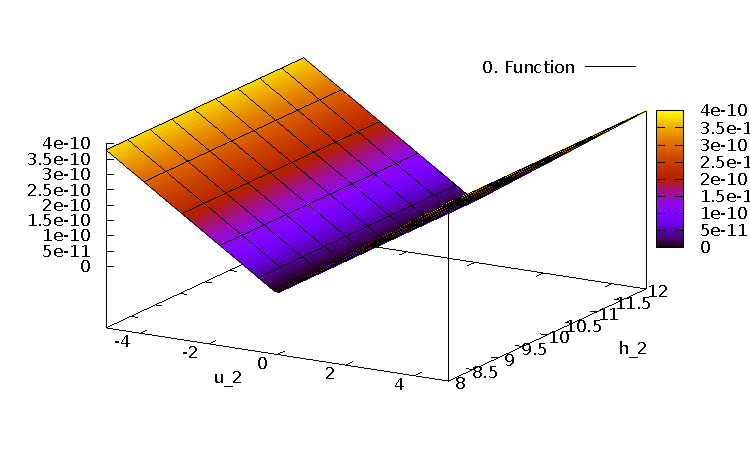
\includegraphics[scale=\zoomfactor]{{{3_punkte_1_geschwindigkeit_verringert/0.0_9.0_0.0_10.0_x_y_0.0_10.0_0.0_10.0_0.0_10.0f0}}} };
%     \fill[white] (.8,1.2) rectangle (1.75,1.5);
%     \node[align=right, text width=3cm] at (.2,1.33) {\textsf{\tiny{Height error}}};
%   \end{tikzpicture}
%   % 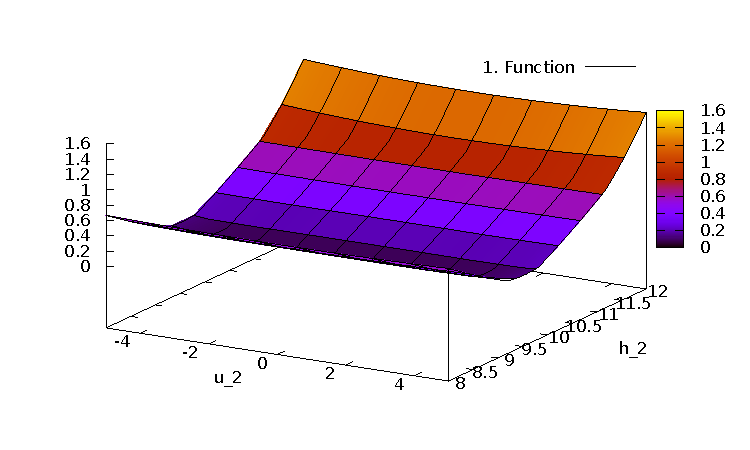
\includegraphics[scale=\zoomfactor]{{{3_punkte_1_geschwindigkeit_verringert/0.0_9.0_0.0_10.0_x_y_0.0_10.0_0.0_10.0_0.0_10.0f1}}} 
% }
\subfigure[Impulse for point $p_2^L$] { 
  %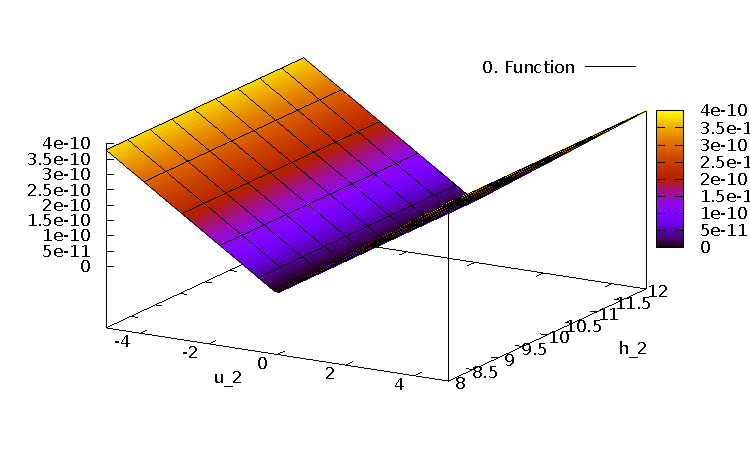
\includegraphics[scale=\zoomfactor]{{{3_punkte_1_geschwindigkeit_verringert/0.0_9.0_0.0_10.0_x_y_0.0_10.0_0.0_10.0_0.0_10.0f0}}} 
  \begin{tikzpicture}
    \node at (0,0) {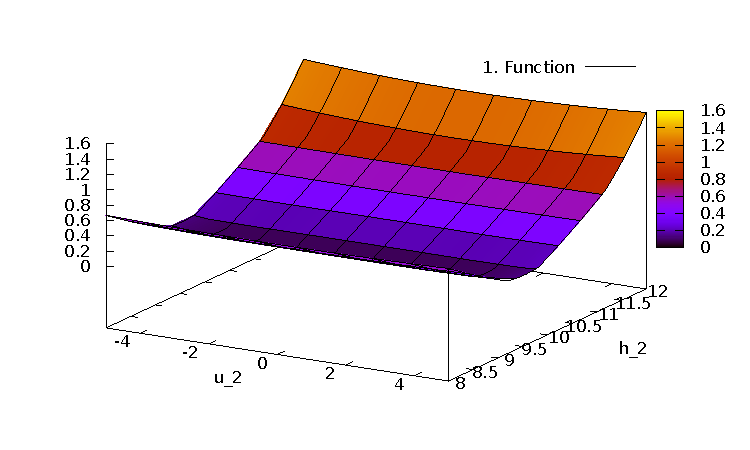
\includegraphics[scale=\zoomfactor]{{{3_punkte_1_geschwindigkeit_verringert/0.0_9.0_0.0_10.0_x_y_0.0_10.0_0.0_10.0_0.0_10.0f1}}} };
    \fill[white] (.8,1.2) rectangle (1.75,1.5);
    \node[align=right, text width=3cm] at (.2,1.33) {\textsf{\tiny{Impulse error}}};
  \end{tikzpicture}
}
\subfigure[Impulse for point $p_3^L$ resp. $p_3^R$] {
  %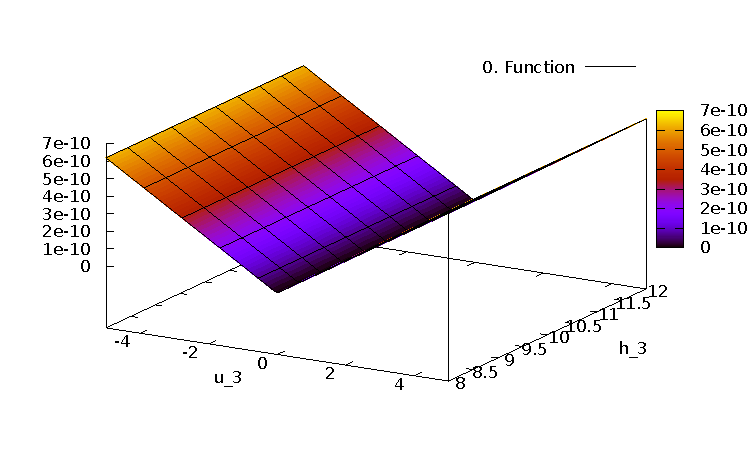
\includegraphics[scale=\zoomfactor]{{{3_punkte_1_geschwindigkeit_verringert/0.0_9.0_0.0_10.0_0.0_10.0_0.0_10.0_x_y_0.0_10.0f0}}} 
  \begin{tikzpicture}
    \node at (0,0) {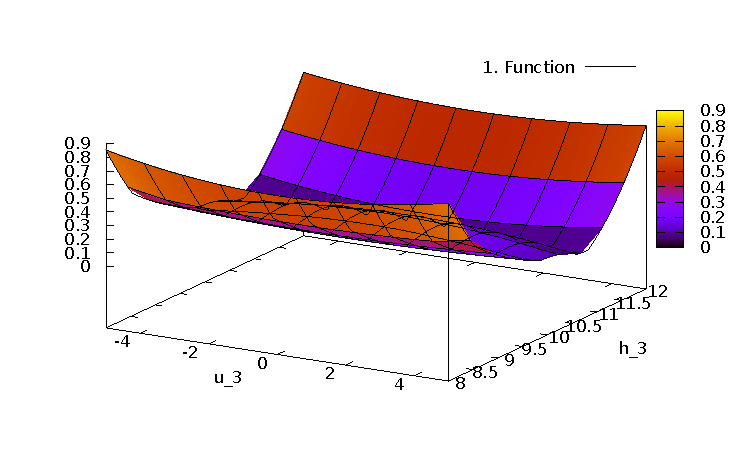
\includegraphics[scale=\zoomfactor]{{{3_punkte_1_geschwindigkeit_verringert/0.0_9.0_0.0_10.0_0.0_10.0_0.0_10.0_x_y_0.0_10.0f1}}} };
    \fill[white] (.8,1.2) rectangle (1.75,1.5);
    \node[align=right, text width=3cm] at (.2,1.33) {\textsf{\tiny{Impulse error}}};
  \end{tikzpicture}
}
\subfigure[Impulse for point $p_1^R$] { 
  %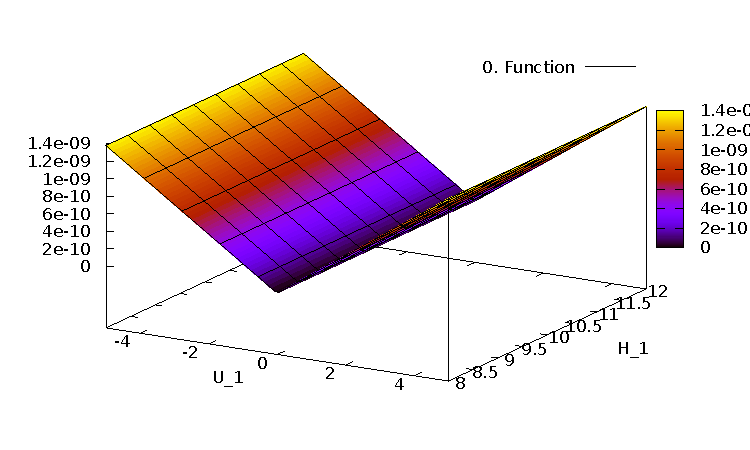
\includegraphics[scale=\zoomfactor]{{{3_punkte_1_geschwindigkeit_verringert/0.0_9.0_x_y_0.0_10.0_0.0_10.0_0.0_10.0_0.0_10.0f0}}} 
  \begin{tikzpicture}
    \node at (0,0) {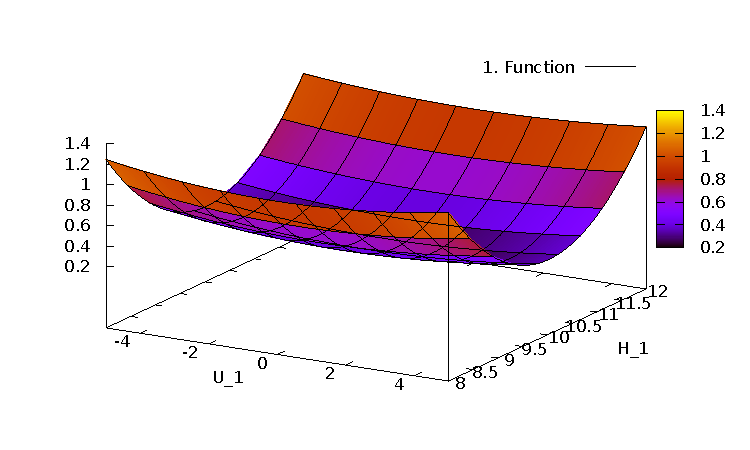
\includegraphics[scale=\zoomfactor]{{{3_punkte_1_geschwindigkeit_verringert/0.0_9.0_x_y_0.0_10.0_0.0_10.0_0.0_10.0_0.0_10.0f1}}} };
    \fill[white] (.8,1.2) rectangle (1.75,1.5);
    \node[align=right, text width=3cm] at (.2,1.33) {\textsf{\tiny{Impulse error}}};
  \end{tikzpicture}
}
\subfigure[Impulse for point $p_2^R$] {
  %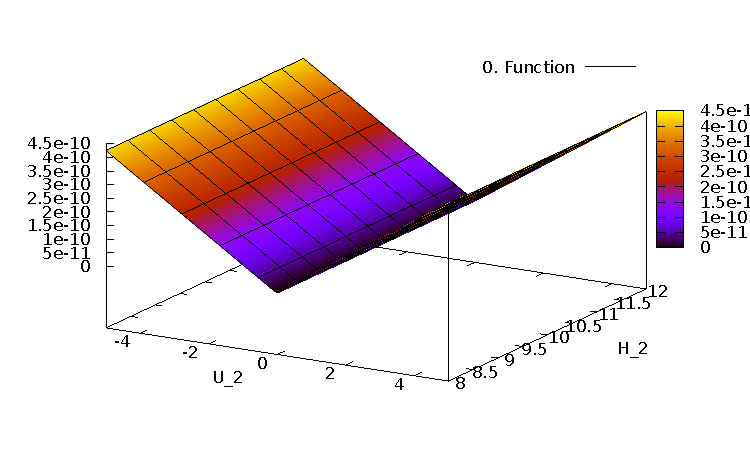
\includegraphics[scale=\zoomfactor]{{{3_punkte_1_geschwindigkeit_verringert/0.0_9.0_0.0_10.0_0.0_10.0_x_y_0.0_10.0_0.0_10.0f0}}} 
  \begin{tikzpicture}
    \node at (0,0) {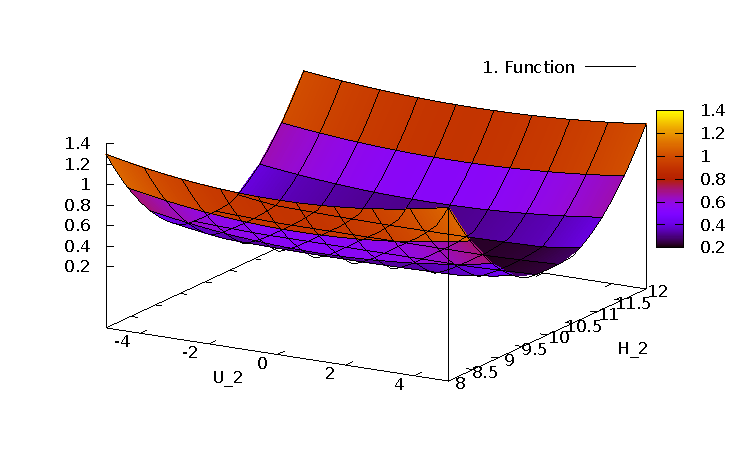
\includegraphics[scale=\zoomfactor]{{{3_punkte_1_geschwindigkeit_verringert/0.0_9.0_0.0_10.0_0.0_10.0_x_y_0.0_10.0_0.0_10.0f1}}} };
    \fill[white] (.8,1.2) rectangle (1.75,1.5);
    \node[align=right, text width=3cm] at (.2,1.33) {\textsf{\tiny{Impulse error}}};
  \end{tikzpicture}
}
% \subfigure[Impulse for point $p_3^R$] {
%   %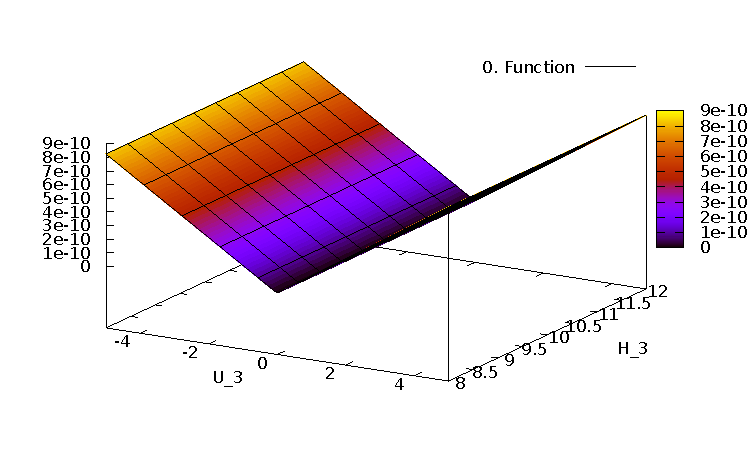
\includegraphics[scale=\zoomfactor]{{{3_punkte_1_geschwindigkeit_verringert/0.0_9.0_0.0_10.0_0.0_10.0_0.0_10.0_0.0_10.0_x_yf0}}} 
%   \begin{tikzpicture}
%     \node at (0,0) {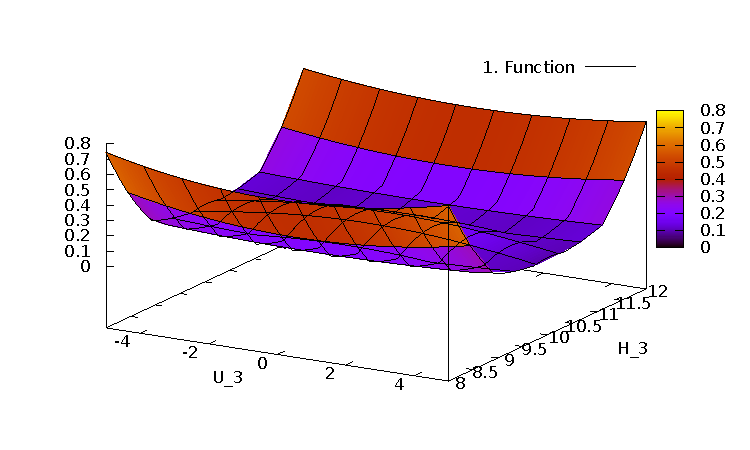
\includegraphics[scale=\zoomfactor]{{{3_punkte_1_geschwindigkeit_verringert/0.0_9.0_0.0_10.0_0.0_10.0_0.0_10.0_0.0_10.0_x_yf1}}} };
%     \fill[white] (.8,1.2) rectangle (1.75,1.5);
%     \node[align=right, text width=3cm] at (.2,1.33) {\textsf{\tiny{Impulse error}}};
%   \end{tikzpicture}
% }
\caption{Three points for each triangle. All points except $p_1$ have height 10, impulse 0. Point $p_1$ is set to $(9,0)$. Since the error in the $h$-component is not very different to the one depicted in subfigure \ref{subfig:height-p1-three-points-height-verringert} (i.e.\,same shape, magnitude $10^{-15}$), we omitted the plots. Especially the plots for $p_2^L$, $p_3^L$ and $p_3^R$ have changed notably.}
\label{fig:three-points-h1-}
\end{figure}

%%% Local Variables:
%%% TeX-master: "../results.tex"
%%% End:

%%% Local Variables:
%%% TeX-master: "../results.tex"
%%% End:


You see the results of this experiment in figure \ref{fig:three-points-h1-}.

Comparing figure \ref{fig:three-points-equal} and \ref{fig:three-points-h1-} it is worth noting that especially the plots for $p_2^L$, $p_3^L$ and $p_3^R$ differ strongly. Additionally, it can be seen that the structure differs as well as the range of the error.

\subsubsection{\texorpdfstring{Decreasing the momentum of $p_1^L$}{Decreasing the momentum of p1L}}
\label{sec:decreasing-momentum-p1}

While we changed the height in subsection \ref{sec:decreasing-height-p1}, we are now going to change the momentum. The results are shown in figure \ref{fig:three-points-u1-}

% 12 variables in here:
% u_1 = -1.0, h_1 = 10.0, U_1 = 0.0, H_1 = 10.0, u_2 = 0.0, h_2 = 10.0, U_2 = 0.0, H_2 = 10.0, u_3 = 0.0, h_3 = 10.0, U_3 = 0.0, H_3 = 10.0
\begin{figure}[h!]
\centering
  % \subfigure[Height and velocity for $p_1$] {
  %   \includegraphics[scale=\zoomfactor]{{{3_punkte_1_impuls_verringert/x_y_0.0_10.0_0.0_10.0_0.0_10.0_0.0_10.0_0.0_10.0f0}}}  
  %   \includegraphics[scale=\zoomfactor]{{{3_punkte_1_impuls_verringert/x_y_0.0_10.0_0.0_10.0_0.0_10.0_0.0_10.0_0.0_10.0f1}}}  
  % }
  \subfigure[Height and velocity for $p_2^L$ resp. $p_2^R$] {
    \label{subfig:p2-height-impulse-three-points-p1-impulse-verringert}
    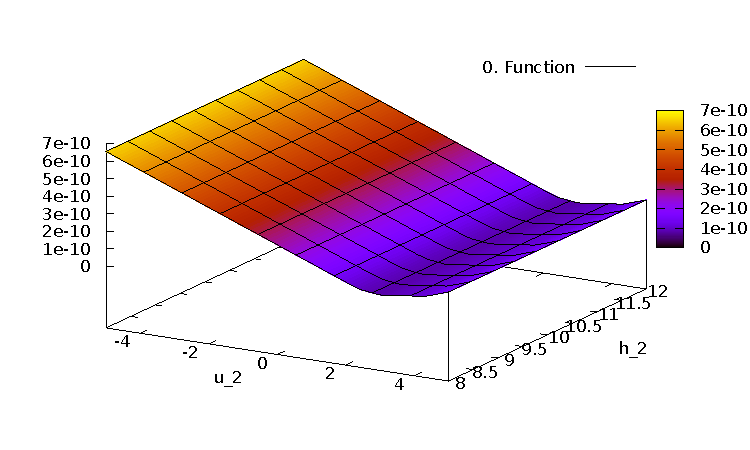
\includegraphics[scale=\zoomfactor]{{{3_punkte_1_impuls_verringert/-1.0_10.0_0.0_10.0_x_y_0.0_10.0_0.0_10.0_0.0_10.0f0}}}  
    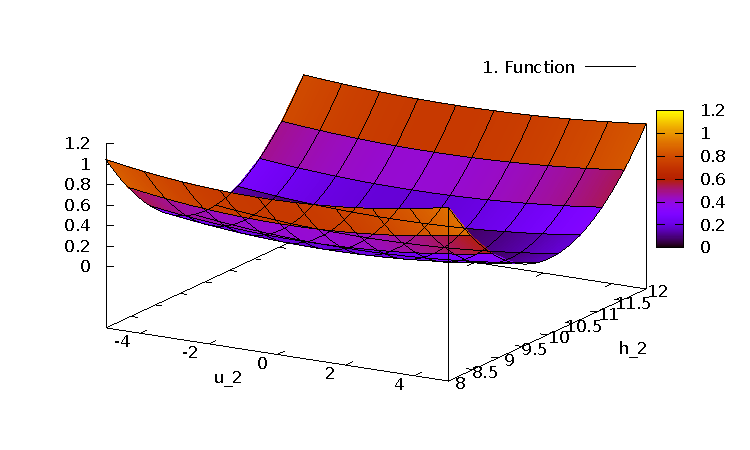
\includegraphics[scale=\zoomfactor]{{{3_punkte_1_impuls_verringert/-1.0_10.0_0.0_10.0_x_y_0.0_10.0_0.0_10.0_0.0_10.0f1}}}  
  }

  \subfigure[Height and velocity for $p_3^L$ res.p $p_3^R$] {
    \label{subfig:p3-height-impulse-three-points-p1-impulse-verringert}
    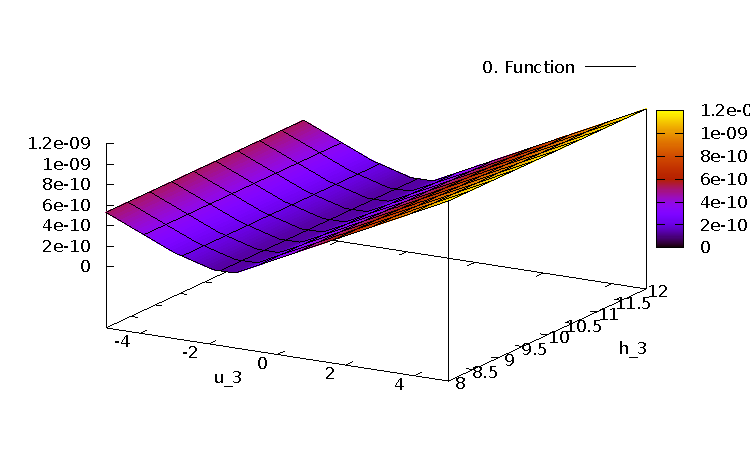
\includegraphics[scale=\zoomfactor]{{{3_punkte_1_impuls_verringert/-1.0_10.0_0.0_10.0_0.0_10.0_0.0_10.0_x_y_0.0_10.0f0}}}  
    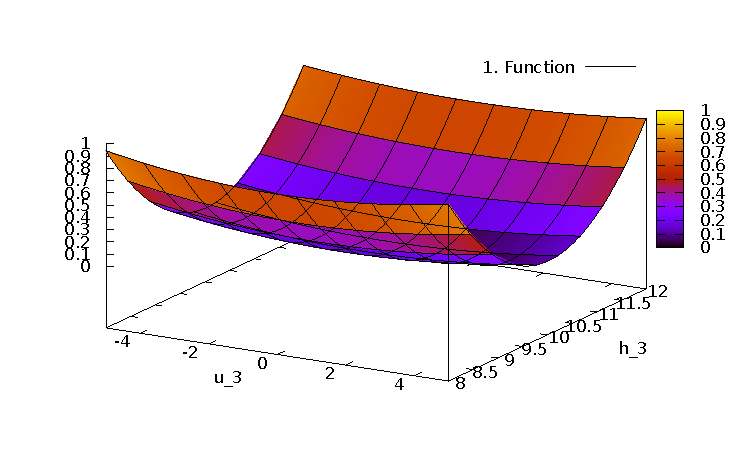
\includegraphics[scale=\zoomfactor]{{{3_punkte_1_impuls_verringert/-1.0_10.0_0.0_10.0_0.0_10.0_0.0_10.0_x_y_0.0_10.0f1}}}  
  }

  \subfigure[Height and velocity for $p_1^R$] {
    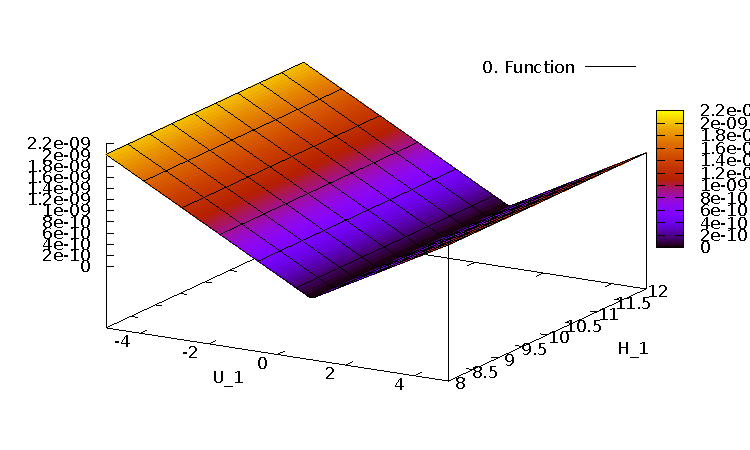
\includegraphics[scale=\zoomfactor]{{{3_punkte_1_impuls_verringert/-1.0_10.0_x_y_0.0_10.0_0.0_10.0_0.0_10.0_0.0_10.0f0}}}  
    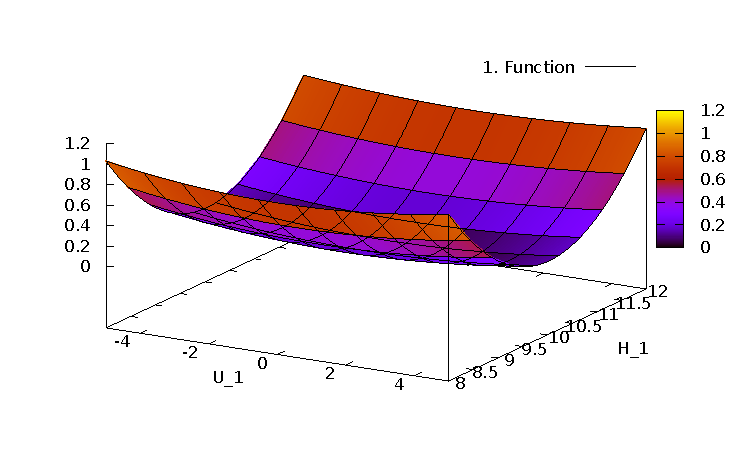
\includegraphics[scale=\zoomfactor]{{{3_punkte_1_impuls_verringert/-1.0_10.0_x_y_0.0_10.0_0.0_10.0_0.0_10.0_0.0_10.0f1}}}  
  }
  % \subfigure[Height and velocity for $p_2^R$] {
  %   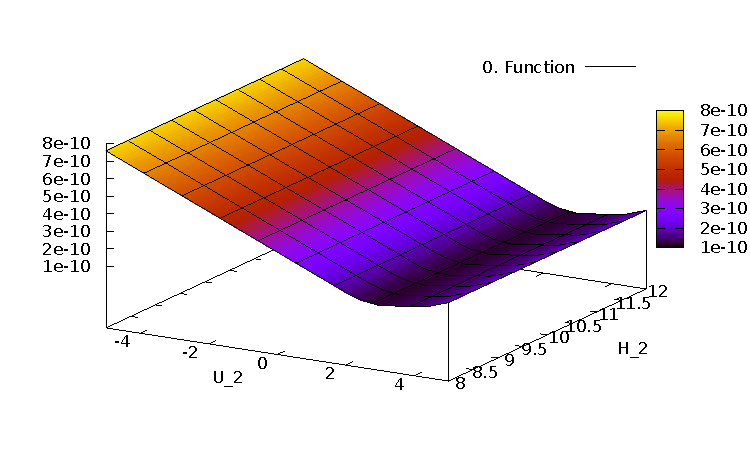
\includegraphics[scale=\zoomfactor]{{{3_punkte_1_impuls_verringert/-1.0_10.0_0.0_10.0_0.0_10.0_x_y_0.0_10.0_0.0_10.0f0}}}  
  %   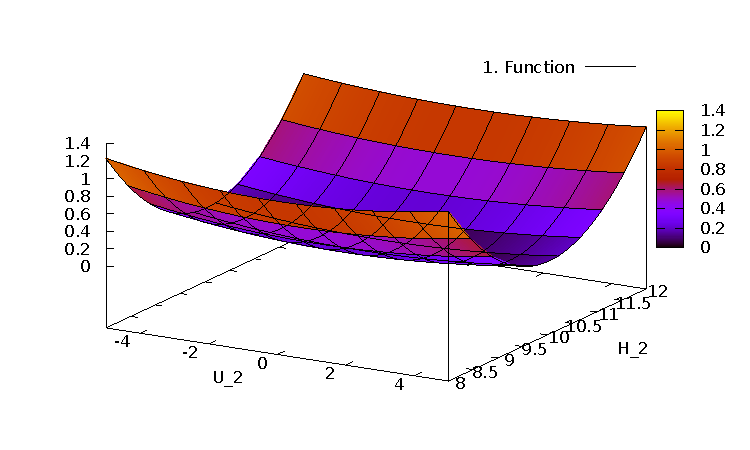
\includegraphics[scale=\zoomfactor]{{{3_punkte_1_impuls_verringert/-1.0_10.0_0.0_10.0_0.0_10.0_x_y_0.0_10.0_0.0_10.0f1}}}  
  % }

  % \subfigure[Height and velocity for $p_3^R$] {
  %   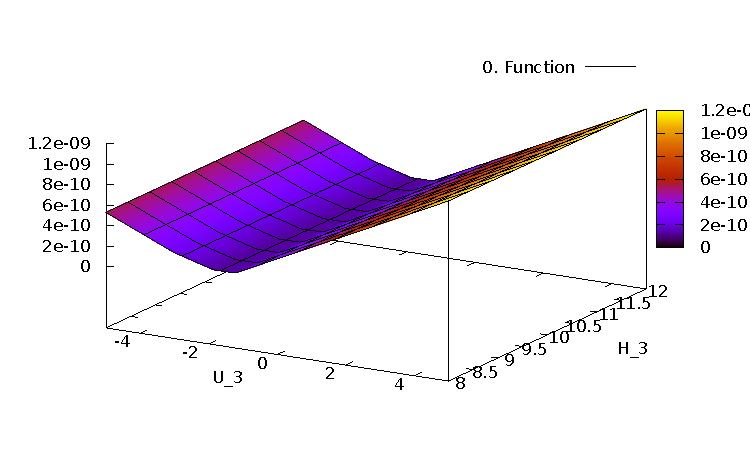
\includegraphics[scale=\zoomfactor]{{{3_punkte_1_impuls_verringert/-1.0_10.0_0.0_10.0_0.0_10.0_0.0_10.0_0.0_10.0_x_yf0}}}  
  %   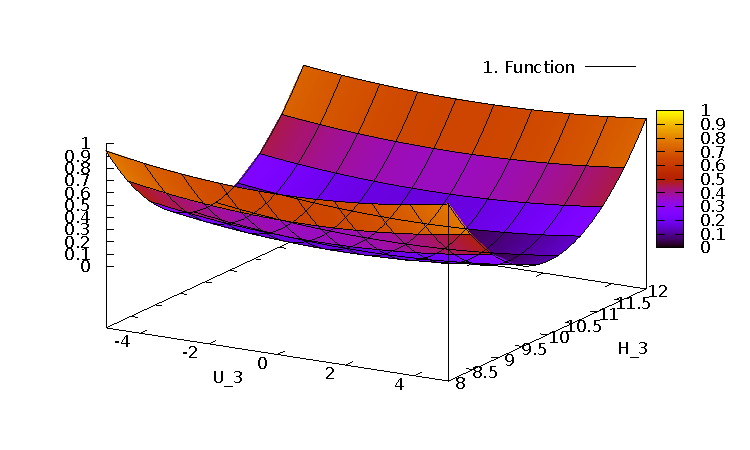
\includegraphics[scale=\zoomfactor]{{{3_punkte_1_impuls_verringert/-1.0_10.0_0.0_10.0_0.0_10.0_0.0_10.0_0.0_10.0_x_yf1}}}  
  % }
  \caption{Three points for each triangle. All points except $p_1$ have height 10, impulse 0. Point $p_1$ is set to $(10,-1)$. Surprisingly, changing the impulse results in  another error concerning the height component more than changing the height component. Subfigure \label{subfig:p2-height-impulse-three-points-p1-impulse-verringert} shows the height and impulse errors as well for $p_2^L$ and $p_2^R$ since the plots (at least) look so similar that they can't be distinguished with the naked eye. Moreover we sum up the plots for points $p_3^L$ and $p_3^R$ in subfigure \ref{subfig:p3-height-impulse-three-points-p1-impulse-verringert} for the same reason.
}
  \label{fig:three-points-u1-}
\end{figure}

%%% Local Variables:
%%% TeX-master: "../results.tex"
%%% End:

%%% Local Variables:
%%% TeX-master: "../results.tex"
%%% End:


\subsubsection{\texorpdfstring{Decreasing the height of $p_2^L$}{Decreasing the height of p2L}}
\label{sec:decreasing-height-p2}

Now we are going to examine if it makes a difference when we decrease the height of another point, namely $p_2^L$. We show the results in figure \ref{fig:three-points-h2-}. In this case, the graphs for points $p_1^L$ and $p_3^L$ in particular are noteworthy.

% 12 variables in here:
% u_1 = 0.0, h_1 = 10.0, U_1 = 0.0, H_1 = 10.0, u_2 = 0.0, h_2 = 9.0, U_2 = 0.0, H_2 = 10.0, u_3 = 0.0, h_3 = 10.0, U_3 = 0.0, H_3 = 10.0
\begin{figure}[h!t]
\centering
  % \subfigure[Height of point $p_1^L$] {
  %   \label{subfig:height-p1-three-points-p2-height-decreased}
  %   \begin{tikzpicture}
  %     \node at (0,0) {\includegraphics[scale=\zoomfactor]{{{3_punkte_2_hoehe_verringert/x_y_0.0_10.0_0.0_9.0_0.0_10.0_0.0_10.0_0.0_10.0f0}}}  };
  %     \fill[white] (.8,1.2) rectangle (1.75,1.5);
  %     \node[align=right, text width=3cm] at (.2,1.33) {\textsf{\tiny{Height error}}};
  %   \end{tikzpicture}
  %   %\includegraphics[scale=\zoomfactor]{{{3_punkte_2_hoehe_verringert/x_y_0.0_10.0_0.0_9.0_0.0_10.0_0.0_10.0_0.0_10.0f1}}}  
  % }
  % \subfigure[Impulse of point $p_2^L$] {
  %   \includegraphics[scale=\zoomfactor]{{{3_punkte_2_hoehe_verringert/0.0_10.0_0.0_10.0_x_y_0.0_10.0_0.0_10.0_0.0_10.0f0}}}  
  %   \includegraphics[scale=\zoomfactor]{{{3_punkte_2_hoehe_verringert/0.0_10.0_0.0_10.0_x_y_0.0_10.0_0.0_10.0_0.0_10.0f1}}}  
  % }

  % \subfigure[Impulse of point $p_3^L$] {
  %   %\includegraphics[scale=\zoomfactor]{{{3_punkte_2_hoehe_verringert/0.0_10.0_0.0_10.0_0.0_9.0_0.0_10.0_x_y_0.0_10.0f0}}}  
  %   \begin{tikzpicture}
  %     \node at (0,0) {\includegraphics[scale=\zoomfactor]{{{3_punkte_2_hoehe_verringert/0.0_10.0_0.0_10.0_0.0_9.0_0.0_10.0_x_y_0.0_10.0f1}}}  };
  %     \fill[white] (.8,1.2) rectangle (1.75,1.5);
  %     \node[align=right, text width=3cm] at (.2,1.33) {\textsf{\tiny{Impulse error}}};
  %   \end{tikzpicture}
  % }
  \subfigure[Impulse of point $p_1^L$ resp. $p_3^L$] {
    %\includegraphics[scale=\zoomfactor]{{{3_punkte_2_hoehe_verringert/x_y_0.0_10.0_0.0_9.0_0.0_10.0_0.0_10.0_0.0_10.0f0}}}  
    \begin{tikzpicture}
      \node at (0,0) {\includegraphics[scale=\zoomfactor]{{{3_punkte_2_hoehe_verringert/x_y_0.0_10.0_0.0_9.0_0.0_10.0_0.0_10.0_0.0_10.0f1}}}  };
      \fill[white] (.8,1.2) rectangle (1.75,1.5);
      \node[align=right, text width=3cm] at (.2,1.33) {\textsf{\tiny{Impulse error}}};
    \end{tikzpicture}
  }
  \subfigure[Impulse of point $p_1^R$ resp. $p_3^R$] {
    %\includegraphics[scale=\zoomfactor]{{{3_punkte_2_hoehe_verringert/0.0_10.0_x_y_0.0_9.0_0.0_10.0_0.0_10.0_0.0_10.0f0}}}  
    \begin{tikzpicture}
      \node at (0,0) {\includegraphics[scale=\zoomfactor]{{{3_punkte_2_hoehe_verringert/0.0_10.0_x_y_0.0_9.0_0.0_10.0_0.0_10.0_0.0_10.0f1}}}  };
      \fill[white] (.8,1.2) rectangle (1.75,1.5);
      \node[align=right, text width=3cm] at (.2,1.33) {\textsf{\tiny{Impulse error}}};
    \end{tikzpicture}
  }
  \subfigure[Impulse of point $p_2^R$] {
    %\includegraphics[scale=\zoomfactor]{{{3_punkte_2_hoehe_verringert/0.0_10.0_0.0_10.0_0.0_9.0_x_y_0.0_10.0_0.0_10.0f0}}}  
    \begin{tikzpicture}
      \node at (0,0) {\includegraphics[scale=\zoomfactor]{{{3_punkte_2_hoehe_verringert/0.0_10.0_0.0_10.0_0.0_9.0_x_y_0.0_10.0_0.0_10.0f1}}}  };
      \fill[white] (.8,1.2) rectangle (1.75,1.5);
      \node[align=right, text width=3cm] at (.2,1.33) {\textsf{\tiny{Impulse error}}};
    \end{tikzpicture}
  }
  % \subfigure[Impulse of point $p_3^R$] {
  %   %\includegraphics[scale=\zoomfactor]{{{3_punkte_2_hoehe_verringert/0.0_10.0_0.0_10.0_0.0_9.0_0.0_10.0_0.0_10.0_x_yf0}}}  
  %   \begin{tikzpicture}
  %     \node at (0,0) {\includegraphics[scale=\zoomfactor]{{{3_punkte_2_hoehe_verringert/0.0_10.0_0.0_10.0_0.0_9.0_0.0_10.0_0.0_10.0_x_yf1}}}  };
  %     \fill[white] (.8,1.2) rectangle (1.75,1.5);
  %     \node[align=right, text width=3cm] at (.2,1.33) {\textsf{\tiny{Impulse error}}};
  %   \end{tikzpicture}
  % }
  \caption{Three points for each triangle. All points except $p_2$ have height 10, impulse 0. Point $p_2$ is set to $(9,0)$.}
  \label{fig:three-points-h2-}
\end{figure}

%%% Local Variables:
%%% TeX-master: "../results.tex"
%%% End:

%%% Local Variables:
%%% TeX-master: "../results.tex"
%%% End:


\subsubsection{\texorpdfstring{Decreasing the momentum of $p_2^L$}{Decreasing the momentum of p2L}}
\label{sec:decreasing-momentum-of-p2}

Decreasing the momentum of point $p_2^L$ results in the plots depicted in figure \ref{fig:three-points-u2-}. In particular, the graphs for $p_1^L$ and $p_3^L$ show significant structural differences.

% 12 variables in here:
% u_1 = 0.0, h_1 = 10.0, U_1 = 0.0, H_1 = 10.0, u_2 = -1.0, h_2 = 10.0, U_2 = 0.0, H_2 = 10.0, u_3 = 0.0, h_3 = 10.0, U_3 = 0.0, H_3 = 10.0
\begin{figure}[h!t]
\centering
  \subfigure[Height for points $p_1^L$ and $p_3^L$ (same for $p_1^R$ and $p_3^R$ respectively).] {
    \includegraphics[scale=\zoomfactor]{{{3_punkte_2_impuls_verringert/x_y_0.0_10.0_-1.0_10.0_0.0_10.0_0.0_10.0_0.0_10.0f0}}}  
    \includegraphics[scale=\zoomfactor]{{{3_punkte_2_impuls_verringert/0.0_10.0_0.0_10.0_-1.0_10.0_0.0_10.0_x_y_0.0_10.0f0}}}  
%    \includegraphics[scale=\zoomfactor]{{{3_punkte_2_impuls_verringert/x_y_0.0_10.0_-1.0_10.0_0.0_10.0_0.0_10.0_0.0_10.0f1}}}  
  }

  \subfigure[Height for points $p_2^L$ and $p_2^R$. Slight difference in scale.] {
    \includegraphics[scale=\zoomfactor]{{{3_punkte_2_impuls_verringert/0.0_10.0_0.0_10.0_x_y_0.0_10.0_0.0_10.0_0.0_10.0f0}}}  
    \includegraphics[scale=\zoomfactor]{{{3_punkte_2_impuls_verringert/0.0_10.0_0.0_10.0_-1.0_10.0_x_y_0.0_10.0_0.0_10.0f0}}}  
%    \includegraphics[scale=\zoomfactor]{{{3_punkte_2_impuls_verringert/0.0_10.0_0.0_10.0_x_y_0.0_10.0_0.0_10.0_0.0_10.0f0}}}  
%    \includegraphics[scale=\zoomfactor]{{{3_punkte_2_impuls_verringert/0.0_10.0_0.0_10.0_0.0_10.0_x_y_0.0_10.0_0.0_10.0f1}}}  
  }

  \subfigure[Impulse for points $p_1^L$ (same for $p_3^L$) and $p_2^L$.] {
    \includegraphics[scale=\zoomfactor]{{{3_punkte_2_impuls_verringert/x_y_0.0_10.0_-1.0_10.0_0.0_10.0_0.0_10.0_0.0_10.0f1}}}  
    \includegraphics[scale=\zoomfactor]{{{3_punkte_2_impuls_verringert/0.0_10.0_0.0_10.0_-1.0_10.0_x_y_0.0_10.0_0.0_10.0f1}}}  
%    \includegraphics[scale=\zoomfactor]{{{3_punkte_2_impuls_verringert/0.0_10.0_0.0_10.0_-1.0_10.0_0.0_10.0_x_y_0.0_10.0f0}}}  
%    \includegraphics[scale=\zoomfactor]{{{3_punkte_2_impuls_verringert/0.0_10.0_0.0_10.0_-1.0_10.0_0.0_10.0_x_y_0.0_10.0f1}}}  
  }

%  \subfigure[Height and impulse for point $P_1$] {
%    \includegraphics[scale=\zoomfactor]{{{3_punkte_2_impuls_verringert/0.0_10.0_x_y_-1.0_10.0_0.0_10.0_0.0_10.0_0.0_10.0f0}}}  
%    \includegraphics[scale=\zoomfactor]{{{3_punkte_2_impuls_verringert/0.0_10.0_x_y_-1.0_10.0_0.0_10.0_0.0_10.0_0.0_10.0f1}}}  
%  }

%  \subfigure[Height and impulse for point $P_2$] {
%    \includegraphics[scale=\zoomfactor]{{{3_punkte_2_impuls_verringert/0.0_10.0_0.0_10.0_-1.0_10.0_x_y_0.0_10.0_0.0_10.0f0}}}  
%    \includegraphics[scale=\zoomfactor]{{{3_punkte_2_impuls_verringert/0.0_10.0_0.0_10.0_-1.0_10.0_x_y_0.0_10.0_0.0_10.0f1}}}  
%  }

%  \subfigure[Height and impulse for point $P_3$] {
%    \includegraphics[scale=\zoomfactor]{{{3_punkte_2_impuls_verringert/0.0_10.0_0.0_10.0_-1.0_10.0_0.0_10.0_0.0_10.0_x_yf0}}}  
%    \includegraphics[scale=\zoomfactor]{{{3_punkte_2_impuls_verringert/0.0_10.0_0.0_10.0_-1.0_10.0_0.0_10.0_0.0_10.0_x_yf1}}}  
%  }
  \caption{Three points for each triangle. All points except $p_2^L$ have height 10, impulse 0. Point $p_2^L$ is set to $(10,-1)$. The resulting error graphs look the same on both triangles for each point ($p_i^L$ and $p_i^R$), with only slight variation in $p_2^L$, due to that point's impulse being different to $p_2^R$'s. The shape between the points is the same, only the scale differs.}
  \label{fig:three-points-u2-}
\end{figure}

%%% Local Variables:
%%% TeX-master: "../results.tex"
%%% End:

%%% Local Variables:
%%% TeX-master: "../results.tex"
%%% End:


\subsection{Random values}
\label{sec:random-values}

The cases we have examined so far were just sample cases to show a qualitative change in error distribution, depending on the variation of certain variables. In reality, variables will differ at several values simultaneously, and are generally not properly aligned. The closest way to simulate that is to assign random values to all the points.

\subsubsection{Two random points}
\label{sec:two-random-points}

We start out with two random points. The results of random assignment of values can be seen in figure \ref{fig:two-points-random}. There are heavy structural differences discernable compared to previous plots. The maximum height error is also a lot higher than it was previously, which is to be expected.

% 8 variables in here:
% u_1 = -2.9, h_1 = 8.8, U_1 = -1.7, H_1 = 10.6, u_2 = -1.4, h_2 = 9.1, U_2 = 3.8, H_2 = 11.6
\begin{figure}[ht]
\centering
  \subfloat[Momentum of point $p_1^L$] {
    %\includegraphics[scale=\zoomfactor]{{{2_random_new/x_y_-1.7_10.6_-1.4_9.1_3.8_11.6f0}}}  
    \begin{tikzpicture}
      \node at (0,0) {\includegraphics[scale=\zoomfactor]{{{2_random_new/x_y_-1.7_10.6_-1.4_9.1_3.8_11.6f1}}}  };
      \fill[white] (.8,1.2) rectangle (1.75,1.5);
      \node[align=right, text width=3cm] at (.2,1.33) {\textsf{\tiny{Momentum error}}};
    \end{tikzpicture}
  }
  \subfloat[Momentum of point $p_2^L$] {
    %\includegraphics[scale=\zoomfactor]{{{2_random_new/-2.9_8.8_-1.7_10.6_x_y_3.8_11.6f0}}}  
    \begin{tikzpicture}
      \node at (0,0) {\includegraphics[scale=\zoomfactor]{{{2_random_new/-2.9_8.8_-1.7_10.6_x_y_3.8_11.6f1}}}  };
      \fill[white] (.8,1.2) rectangle (1.75,1.5);
      \node[align=right, text width=3cm] at (.2,1.33) {\textsf{\tiny{Momentum error}}};
    \end{tikzpicture}
  }

  \subfloat[Momentum of point $p_1^R$] {
    %\includegraphics[scale=\zoomfactor]{{{2_random_new/-2.9_8.8_x_y_-1.4_9.1_3.8_11.6f0}}}  
    \begin{tikzpicture}
      \node at (0,0) {\includegraphics[scale=\zoomfactor]{{{2_random_new/-2.9_8.8_x_y_-1.4_9.1_3.8_11.6f1}}}  };
      \fill[white] (.8,1.2) rectangle (1.75,1.5);
      \node[align=right, text width=3cm] at (.2,1.33) {\textsf{\tiny{Momentum error}}};
    \end{tikzpicture}
  }
  \subfloat[Momentum of point $p_2^R$] {
    %\includegraphics[scale=\zoomfactor]{{{2_random_new/-2.9_8.8_-1.7_10.6_-1.4_9.1_x_yf0}}}  
    \begin{tikzpicture}
      \node at (0,0) {\includegraphics[scale=\zoomfactor]{{{2_random_new/-2.9_8.8_-1.7_10.6_-1.4_9.1_x_yf1}}}  };
      \fill[white] (.8,1.2) rectangle (1.75,1.5);
      \node[align=right, text width=3cm] at (.2,1.33) {\textsf{\tiny{Momentum error}}};
    \end{tikzpicture}
  }
  \caption{Two points for each triangle. Values for the points are: $u_1^L = -2.9, h_1^L = 8.8, u_1^R = -1.7, h_1^R = 10.6, u_2^L = -1.4, h_2^L = 9.1, u_2^R = 3.8, h_2^r = 11.6$.}
  \label{fig:two-points-random}
\end{figure}

%%% Local Variables:
%%% TeX-master: "../results.tex"
%%% End:

%%% Local Variables:
%%% TeX-master: "../results.tex"
%%% End:


\subsubsection{Three random points}
\label{sec:three-random-points}

The same calculations for three random points is shown in figure \ref{fig:three-points-random}. Again, it differs strongly from figure \ref{fig:three-points-equal}, where we set all points to the same value.

% 12 variables in here:
% u_1 = 3.9, h_1 = 11.0, U_1 = -1.3, H_1 = 11.3, u_2 = 1.7, h_2 = 8.6, U_2 = 3.5, H_2 = 11.9, u_3 = -3.2, h_3 = 11.4, U_3 = -3.8, H_3 = 8.7
\begin{figure}[h!t]
\centering
  \subfigure[Impulse error for point $p_1^L$] {
    % \begin{tikzpicture}
    %   \node at (0,0) {\includegraphics[scale=\zoomfactor]{{{3_random_new/x_y_-1.3_11.3_1.7_8.6_3.5_11.9_-3.2_11.4_-3.8_8.7f0}}}  };
    %   \fill[white] (.8,1.2) rectangle (1.75,1.5);
    %   \node[align=right, text width=3cm] at (.2,1.33) {\textsf{\tiny{Height error}}};
    % \end{tikzpicture}
    \begin{tikzpicture}
      \node at (0,0) {\includegraphics[scale=\zoomfactor]{{{3_random_new/x_y_-1.3_11.3_1.7_8.6_3.5_11.9_-3.2_11.4_-3.8_8.7f1}}}  };
      \fill[white] (.8,1.2) rectangle (1.75,1.5);
      \node[align=right, text width=3cm] at (.2,1.33) {\textsf{\tiny{Impulse error}}};
    \end{tikzpicture}
  }
  % \subfigure[Height and Impulse for point $p_2^L$] {
  %   \includegraphics[scale=\zoomfactor]{{{3_random_new/3.9_11.0_-1.3_11.3_x_y_3.5_11.9_-3.2_11.4_-3.8_8.7f0}}}  
  %   \includegraphics[scale=\zoomfactor]{{{3_random_new/3.9_11.0_-1.3_11.3_x_y_3.5_11.9_-3.2_11.4_-3.8_8.7f1}}}  
  % }
  \subfigure[Impulse error for point $p_3^L$] {
    % \begin{tikzpicture}
    %   \node at (0,0) {\includegraphics[scale=\zoomfactor]{{{3_random_new/3.9_11.0_-1.3_11.3_1.7_8.6_3.5_11.9_x_y_-3.8_8.7f0}}}  };
    %   \fill[white] (.8,1.2) rectangle (1.75,1.5);
    %   \node[align=right, text width=3cm] at (.2,1.33) {\textsf{\tiny{Height error}}};
    % \end{tikzpicture}
    \begin{tikzpicture}
      \node at (0,0) {\includegraphics[scale=\zoomfactor]{{{3_random_new/3.9_11.0_-1.3_11.3_1.7_8.6_3.5_11.9_x_y_-3.8_8.7f1}}}  };
      \fill[white] (.8,1.2) rectangle (1.75,1.5);
      \node[align=right, text width=3cm] at (.2,1.33) {\textsf{\tiny{Impulse error}}};
    \end{tikzpicture}
  }

  \subfigure[Impulse error for point $p_1^R$] {
    % \includegraphics[scale=\zoomfactor]{{{3_random_new/3.9_11.0_x_y_1.7_8.6_3.5_11.9_-3.2_11.4_-3.8_8.7f0}}}  
    \begin{tikzpicture}
      \node at (0,0) {\includegraphics[scale=\zoomfactor]{{{3_random_new/3.9_11.0_x_y_1.7_8.6_3.5_11.9_-3.2_11.4_-3.8_8.7f1}}}  };
      \fill[white] (.8,1.2) rectangle (1.75,1.5);
      \node[align=right, text width=3cm] at (.2,1.33) {\textsf{\tiny{Impulse error}}};
    \end{tikzpicture}
  }
  \subfigure[Impulse error for point $p_2^R$] {
    % \includegraphics[scale=\zoomfactor]{{{3_random_new/3.9_11.0_-1.3_11.3_1.7_8.6_x_y_-3.2_11.4_-3.8_8.7f0}}}  
    \begin{tikzpicture}
      \node at (0,0) {\includegraphics[scale=\zoomfactor]{{{3_random_new/3.9_11.0_-1.3_11.3_1.7_8.6_x_y_-3.2_11.4_-3.8_8.7f1}}}  };
      \fill[white] (.8,1.2) rectangle (1.75,1.5);
      \node[align=right, text width=3cm] at (.2,1.33) {\textsf{\tiny{Impulse error}}};
    \end{tikzpicture}
  }

  % \subfigure[Height and Impulse for point $p_3^R$] {
  %   \includegraphics[scale=\zoomfactor]{{{3_random_new/3.9_11.0_-1.3_11.3_1.7_8.6_3.5_11.9_-3.2_11.4_x_yf0}}}  
  %   \includegraphics[scale=\zoomfactor]{{{3_random_new/3.9_11.0_-1.3_11.3_1.7_8.6_3.5_11.9_-3.2_11.4_x_yf1}}}  
  % }
\caption{Selected plots when choosing the height and impulse of three points randomly. Height and impulse data for these plots: $u_1^L = 3.9, h_1^L = 11.0, u_1^R = -1.3, h_1^R = 11.3, u_2^L = 1.7, h_2^L = 8.6, u_2^R = 3.5, h_2^R = 11.9, u_3^L = -3.2, h_3^L = 11.4, u_3^R = -3.8, h_3^R = 8.7$}
\label{fig:three-points-random}
\end{figure}

%%% Local Variables:
%%% TeX-master: "../results.tex"
%%% End:

%%% Local Variables:
%%% TeX-master: "../results.tex"
%%% End:


\section{Equidistant distribution of support points}
\label{sec:equidistant-distribution-of-support-points}

When one considers the figures depicted in section \ref{sec:results}, it seems intuitive to assume that the error grows if the values for $h$ and $u$ diverge further from the average.

One suspicion that could explain that intuition is that because of the fact that the polynomials $N\left(x\right)$ and $N^\prime\left(x\right)$ generally diverge towards the borders of $[0,1]$.

So we chose the support points equidistant over the interval $[0,1]$ and conducted some experiments. When we choose the support points equidistant over this interval, 0 and 1 are support points and we can be sure that $N\left(x\right)$ and $N^\prime\left(x\right)$ coincide at the values 0 and 1 (i.e.\,$N\left(0\right)=N^\prime\left(0\right)$ and $N\left(1\right)=N^\prime\left(1\right)$).

In this section, we show some results that were obtained by choosing the support points equidistant along the edge.

\subsection{Three fixed support points}
\label{sec:equidistant-three-fixed}

We started as in section \ref{sec:setting-all-support-points-to-the-same-value} and set all support points to $
\begin{pmatrix}
  10 \\ 0
\end{pmatrix}$. You can see the resulting plots in figure \ref{fig:three-equidistant-all-fixed}. And while the results do differ from the ones depicted in figure \ref{fig:three-points-equal}, where we examined the same situation for the Gaussian quadrature support points, the shape of the plots still looks very similar. The range of the error differs only slightly as well.

% 12 variables in here:
% u_1 = 0.0, h_1 = 10.0, U_1 = 0.0, H_1 = 10.0, u_2 = 0.0, h_2 = 10.0, U_2 = 0.0, H_2 = 10.0, u_3 = 0.0, h_3 = 10.0, U_3 = 0.0, H_3 = 10.0
\begin{figure}[h!t]
\centering
  \subfigure[Impulse error of $p_1^L$, $p_1^R$, $p_3^L$ resp. $p_3^R$ for equidistant support points at $\{0, \frac{1}{2}, 1\}$] {
    %\includegraphics[scale=\zoomfactor]{{{3_punkte_equidist_alles_gleich/x_y_0.0_10.0_0.0_10.0_0.0_10.0_0.0_10.0_0.0_10.0f0}}}  
    \begin{tikzpicture}
      \node at (0,0) {\includegraphics[scale=\zoomfactor]{{{3_punkte_equidist_alles_gleich/x_y_0.0_10.0_0.0_10.0_0.0_10.0_0.0_10.0_0.0_10.0f1}}}  };
      \fill[white] (.8,1.2) rectangle (1.75,1.5);
      \node[align=right, text width=3cm] at (.2,1.33) {\textsf{\tiny{Impulse error}}};
    \end{tikzpicture}
  }
  \hspace{.3cm}
  \subfigure[Impulse error of $p_2^L$ resp. $p_2^R$ for equidistant support points at $\{0, \frac{1}{2}, 1\}$] {
    %\includegraphics[scale=\zoomfactor]{{{3_punkte_equidist_alles_gleich/0.0_10.0_0.0_10.0_x_y_0.0_10.0_0.0_10.0_0.0_10.0f0}}}  
    \begin{tikzpicture}
      \node at (0,0) {\includegraphics[scale=\zoomfactor]{{{3_punkte_equidist_alles_gleich/0.0_10.0_0.0_10.0_x_y_0.0_10.0_0.0_10.0_0.0_10.0f1}}}  };
      \fill[white] (.8,1.2) rectangle (1.75,1.5);
      \node[align=right, text width=3cm] at (.2,1.33) {\textsf{\tiny{Impulse error}}};
    \end{tikzpicture}
  }
  % \subfigure[Height and impulse of $p_3^L$ resp. $p_3^R$.] {
  %   %\includegraphics[scale=\zoomfactor]{{{3_punkte_equidist_alles_gleich/0.0_10.0_0.0_10.0_0.0_10.0_0.0_10.0_x_y_0.0_10.0f0}}}  
  %   \includegraphics[scale=\zoomfactor]{{{3_punkte_equidist_alles_gleich/0.0_10.0_0.0_10.0_0.0_10.0_0.0_10.0_x_y_0.0_10.0f1}}}  
  % }
  % \subfigure[Height and impulse of $p_1^R$.] {
  %   %\includegraphics[scale=\zoomfactor]{{{3_punkte_equidist_alles_gleich/0.0_10.0_x_y_0.0_10.0_0.0_10.0_0.0_10.0_0.0_10.0f0}}}  
  %   \includegraphics[scale=\zoomfactor]{{{3_punkte_equidist_alles_gleich/0.0_10.0_x_y_0.0_10.0_0.0_10.0_0.0_10.0_0.0_10.0f1}}}  
  % }
  % \subfigure[Height and impulse of $p_2^R$.] {
  %   %\includegraphics[scale=\zoomfactor]{{{3_punkte_equidist_alles_gleich/0.0_10.0_0.0_10.0_0.0_10.0_x_y_0.0_10.0_0.0_10.0f0}}}  
  %   \includegraphics[scale=\zoomfactor]{{{3_punkte_equidist_alles_gleich/0.0_10.0_0.0_10.0_0.0_10.0_x_y_0.0_10.0_0.0_10.0f1}}}  
  % }
  % \subfigure[Height and impulse of $p_3^R$.] {
  %   %\includegraphics[scale=\zoomfactor]{{{3_punkte_equidist_alles_gleich/0.0_10.0_0.0_10.0_0.0_10.0_0.0_10.0_0.0_10.0_x_yf0}}}  
  %   \includegraphics[scale=\zoomfactor]{{{3_punkte_equidist_alles_gleich/0.0_10.0_0.0_10.0_0.0_10.0_0.0_10.0_0.0_10.0_x_yf1}}}  
  % }

  \subfigure[Impulse error for point $p_1^L$, $p_3^L$, $p_1^R$ resp. $p_3^R$ for support points at $\{-\frac{\sqrt{15}}{10}\pm\frac{1}{2}, 0\}$] {
    % \begin{tikzpicture}
    %   \node at (0,0) {\includegraphics[scale=\zoomfactor]{{{3_punkte_gleich/x_y_0.0_10.0_0.0_10.0_0.0_10.0_0.0_10.0_0.0_10.0f0}}}   };
    %   \fill[white] (.8,1.2) rectangle (1.75,1.5);
    %   \node[align=right, text width=3cm] at (.2,1.33) {\textsf{\tiny{Height error}}};
    % \end{tikzpicture}
    \begin{tikzpicture}
      \node at (0,0) {\includegraphics[scale=\zoomfactor]{{{3_punkte_gleich/x_y_0.0_10.0_0.0_10.0_0.0_10.0_0.0_10.0_0.0_10.0f1}}}   };
      \fill[white] (.8,1.2) rectangle (1.75,1.5);
      \node[align=right, text width=3cm] at (.2,1.33) {\textsf{\tiny{Impulse error}}};
    \end{tikzpicture}
  }
  \hspace{.3cm}
  \subfigure[Impulse error for point $p_2^L$ resp. $p_2^R$ for support points at $\{-\frac{\sqrt{15}}{10}\pm\frac{1}{2}, 0\}$] {
    % \begin{tikzpicture}
    %   \node at (0,0) {\includegraphics[scale=\zoomfactor]{{{3_punkte_gleich/0.0_10.0_0.0_10.0_x_y_0.0_10.0_0.0_10.0_0.0_10.0f0}}}   };
    %   \fill[white] (.8,1.2) rectangle (1.75,1.5);
    %   \node[align=right, text width=3cm] at (.2,1.33) {\textsf{\tiny{Height error}}};
    % \end{tikzpicture}
    \begin{tikzpicture}
      \node at (0,0) {\includegraphics[scale=\zoomfactor]{{{3_punkte_gleich/0.0_10.0_0.0_10.0_x_y_0.0_10.0_0.0_10.0_0.0_10.0f1}}}   };
      \fill[white] (.8,1.2) rectangle (1.75,1.5);
      \node[align=right, text width=3cm] at (.2,1.33) {\textsf{\tiny{Impulse error}}};
    \end{tikzpicture}
  }
\caption{Three support points. Coordinates of points are (10,0). We compare equidistant support points to support points obtained from Gaussian quadrature.}
\label{fig:three-equidistant-all-fixed}
\end{figure}

%%% Local Variables:
%%% TeX-master: "../results.tex"
%%% End:

%%% Local Variables:
%%% TeX-master: "../results.tex"
%%% End:


\section{Conclusions from the things seen}
\label{sec:conslusions}

What all plots have in common is the fact that it looks as if towards the boundarys the error grows. However, trying to determine an exact formula for the deviation is impracticle due to the amount of variables that all interact with each other, and may even be impossible.

\clearpage{}

\part{Stiffness matrix accuracy analysis}
\label{part:stiffness-matrix}

\emph{Remark:} Since the following part contains a myriad of mathematical symbols, we encourage you to have a copy of the cheat sheet from section \ref{sec:cheat-sheet-stiffn} on page \pageref{sec:cheat-sheet-stiffn}.

\section{Sum approximation vs. exact solution}
\label{sec:point-wise-appr-vs-exact-solution-intro}

While deriving the equations necessary for our calculations, we introduced several approximations. One of them was the approximation of the combination of various sums, as presented in the calculation of the stiffness matrix in section \ref{sec:stiffness-second-line}, in particular in the equations (\ref{eq:third-integral-second-line-1}) and (\ref{eq:third-integral-second-line-2}). For the second line (i.e. for the $u_x$ component), we had:

\begin{eqnarray}
  \label{eq:third-integral-second-line-1-analysis-part}
  \int_T F_2(\mathbf{q}) \cdot \nabla \phi \, dT & = &
  \int_T
  \begin{pmatrix}
    \frac{u_x^2}{h} + \frac{1}{2} g h^2 \\ \frac{u_x u_y}{h}
  \end{pmatrix}
  \cdot \nabla \phi_i \, dT \\
  \label{eq:third-integral-second-line-2-analysis-part}
  & \approx &
  \int_T
  \begin{pmatrix}
    \sum_{j=1}^n \left(\frac{u_{x,j}^2}{h_j^2} + \frac{1}{2} g h_j^2\right) \phi_j \\
    \sum_{j=1}^n \left(\frac{u_{x,j} u_{y,j}}{h_j}\right) \phi_j \\
  \end{pmatrix}
  \cdot
  \begin{pmatrix}
    \pd{\phi_i}{x} \\
    \pd{\phi_i}{y}
  \end{pmatrix} dT \\
  & = & \nonumber \sum_{j=1}^n \left(\frac{u_{x,j}^2}{h_j^2} + \frac{1}{2} g h_j^2\right) \int_T \phi_j \pd{\phi_i}{x} \, dT \\
  & {} & + \nonumber \sum_{j=1}^n \left(\frac{u_{x,j} u_{y,j}}{h_j}\right) \int_T \phi_j \pd{\phi_i}{y} \, dT
\end{eqnarray}

The equation for the $u_y$ component was analogous:

\begin{eqnarray*}
  \int_T F_3\left(\mathbf{q}\right) \cdot \nabla \phi \, dT & = &
  \int_T
  \begin{pmatrix}
    \frac{u_x u_y}{h} \\ \frac{u_y^2}{h} + \frac{1}{2} g h^2
  \end{pmatrix}
  \cdot \nabla \phi_i \, dT \\
  & \approx & \int_T
  \begin{pmatrix}
    \sum_{j=1}^n \left(\frac{u_{x,j} u_{y,j}}{h_j}\right) \phi_j \\
    \sum_{j=1}^n \left(\frac{u_{y,j}^2}{h_j^2} + \frac{1}{2} g h_j^2\right) \phi_j \\
  \end{pmatrix}
  \cdot
  \begin{pmatrix}
    \pd{\phi_i}{x} \\
    \pd{\phi_i}{y}
  \end{pmatrix} dT \\
  & = & \sum_{j=1}^n \left(\frac{u_{x,j} u_{y,j}}{h_j}\right) \int_T \phi_j \pd{\phi_i}{x} \, dT \\
  & {} & + \sum_{j=1}^n \left(\frac{u_{y,j}^2}{h_j^2} + \frac{1}{2} g h_j^2\right) \int_T \phi_j \pd{\phi_i}{y} \, dT
\end{eqnarray*}

We will introduce this notation to refer to the approximated integrand:

\begin{equation}
  \label{eq:point-wise-approx-result-second-line}
  \overline{F}_2(\mathbf{q}) \cdot \nabla \phi =
  \begin{pmatrix}
    \sum_{j=1}^n \left(\frac{u_{x,j}^2}{h_j^2} + \frac{1}{2} g h_j^2\right) \phi_j \\
    \sum_{j=1}^n \left(\frac{u_{x,j} u_{y,j}}{h_j}\right) \phi_j \\
  \end{pmatrix}
  \cdot
  \begin{pmatrix}
    \pd{\phi_i}{x} \\
    \pd{\phi_i}{y}
  \end{pmatrix}
\end{equation}

\begin{equation}
  \label{eq:point-wise-approx-result-third-line}
  \overline{F}_3(\mathbf{q}) \cdot \nabla \phi =
  \begin{pmatrix}
    \sum_{j=1}^n \left(\frac{u_{x,j} u_{y,j}}{h_j}\right) \phi_j \\
    \sum_{j=1}^n \left(\frac{u_{y,j}^2}{h_j^2} + \frac{1}{2} g h_j^2\right) \phi_j \\
  \end{pmatrix}
  \cdot
  \begin{pmatrix}
    \pd{\phi_i}{x} \\
    \pd{\phi_i}{y}
  \end{pmatrix}
\end{equation}

As mentioned in section \ref{sec:stiffness-second-line}, we approximated the rational function containing a product of sums. This approximation implies some loss of precision. We will now examine the difference between the exact\footnote{Exact in the sense that we substitute $h$ by $\sum_{j=1}^n \phi_j \cdot h_j$ and substitute $u_x$ and $u_y$ accordingly.} and our approximate solution and try to analyze its validity.

We do so by exemplarily examining the third component and try to calculate its exact value:

\begin{eqnarray*}
  \int_T F_2\left(\mathbf{q}\right) \cdot \nabla \phi \, dT & = &
  \int_T
  \begin{pmatrix}
    \frac{u_x u_y}{h} \\ \frac{u_y^2}{h} + \frac{1}{2} g h^2
  \end{pmatrix}
  \cdot \nabla \phi_i \, dT \\
  & \approx & \int_T
  \begin{pmatrix}
    \frac{(\sum_{j=1}^n \phi_j u_{x,j}) \cdot (\sum_{j=1}^n \phi_j u_{y,j})}{\sum_{j=1}^n \phi_j h_j} \\ \frac{(\sum_{j=1}^n \phi_j u_{y,j})^2}{\sum_{j=1}^n \phi_j h_j} + \frac{1}{2} g (\sum_{j=1}^n \phi_j h_j)^2
  \end{pmatrix}
  \cdot \nabla \phi_i \, dT = \\
  & = &
  \frac{(\sum_{j=1}^n \phi_j u_{x,j}) \cdot (\sum_{j=1}^n \phi_j u_{y,j})}{\sum_{j=1}^n \phi_j h_j} \cdot \pd{\phi_i}{x} + \\
  & & \left( \frac{(\sum_{j=1}^n \phi_j u_{y,j})^2}{\sum_{j=1}^n \phi_j h_j} + \frac{1}{2} g (\sum_{j=1}^n \phi_j h_j)^2 \right) \cdot \pd{\phi_i}{y}
\end{eqnarray*}

While we approximate here as well, it's the point-wise sampling approximation and is used in both cases, as it's impossible to determine the exact value for a continuous area.

These terms are become huge and difficult to handle manually (as well as expensive to compute automatically). We will introduce three shorthand notations for the three components of $\mathbf{q}$:

\begin{equation}
  \label{eq:substitutions-for-all-components-with-hat}
  \widehat{h} := \sum_{j=1}^n \phi_j h_j \quad
  \widehat{u}_y := \sum_{j=1}^n \phi_j u_{y,j} \quad
  \widehat{u}_x := \sum_{j=1}^n \phi_j u_{x,j}
\end{equation}

Similarily to before, we can introduce a hat notation to signal the summation of the individual components, only this time we define it for the entire integrand. Doing that, we can simply the above term:

\begin{equation}
  \label{eq:stiffness-analysis-third-line-exact-approx-simple}
  \widehat{F}_3(\mathbf{q}) \cdot \nabla \phi=
  \frac{\widehat{u}_x \cdot \widehat{u}_y }{\widehat{h}} \cdot \pd{\phi_i}{x} +
  \left( \frac{\widehat{u}_y^2}{\widehat{h}} + \frac{1}{2} g \widehat{h}^2 \right) \cdot \pd{\phi_i}{y}
\end{equation}

Analogously, we define this for the second component:

\begin{equation}
  \label{eq:stiffness-analysis-second-line-exact-approx-simple}
  \widehat{F}_2(\mathbf{q}) \cdot \nabla \phi =
  \left( \frac{\widehat{u}_x^2}{\widehat{h}} + \frac{1}{2} g \widehat{h}^2 \right) \cdot \pd{\phi_i}{x} +
  \frac{\widehat{u}_x \cdot \widehat{u}_y }{\widehat{h}} \cdot \pd{\phi_i}{y}
\end{equation}

\subsection{Comparison of exact and approximative solution}

We have now derived an exact solution ($\widehat{F}_2(\mathbf{q}) \cdot \nabla \phi$ and $\widehat{F}_3(\mathbf{q}) \cdot \nabla \phi$) and one that uses an approximation for the rational fraction ($\overline{F}_2(\mathbf{q}) \cdot \nabla \phi$ and $\overline{F}_3(\mathbf{q}) \cdot \nabla \phi$ respectively). We now compare these two with the $L_1$ norm, as we did in the previous part. For that we take the absolute value of the difference, and then integrate over the domain. We do this once for each component, hence we get these two terms called $SE_x$ and $SE_y$ respectively:

\begin{eqnarray*}
  SE_x := \int_T \left| \overline{F}_2(\mathbf{q}) \cdot \nabla \phi - \widehat{F}_2(\mathbf{q}) \cdot \nabla \phi \right| \, dT, \quad
  SE_y := \int_T \left| \overline{F}_3(\mathbf{q}) \cdot \nabla \phi - \widehat{F}_3(\mathbf{q}) \cdot \nabla \phi \right| \, dT
\end{eqnarray*}

These terms could be simplified a bit further (for example by factoring out $\nabla \phi$), but since the terms are rather complicated anyway, we omit such manual simplifications and delegate tasks of this kind to Maple (or any equivalent computer algebra system).

As you can see, computing these terms involves the terms $\phi$ that acts as a representative for \emph{one} of the basis functions $\phi_1,\dots,\phi_n$. That means we get these two error terms ($SE_x$, $SE_y$) for \emph{each} basis function. To distinguish these two, we add superscript indices to indicate the underlying basis function: $SE^i=
\begin{pmatrix}
  SE_x^i \\ SE_y^i
\end{pmatrix}$ is the error term for basis function $\phi_i$.

\subsection{\texorpdfstring{What does $SE$ mean?}{What does SE mean?}}
\label{sec:stiffness-analysis-what-does-se-mean}

Each component of $SE$ describes the deviation between two functions (namely the exact solution and the point-wise approximation). Due to comparing norms for our desired terms, the only thing one can say for sure is that if $SE$ is zero in either component, then the compared functions in that component are equal, i.e. then we have no error at all.

On the other hand, the greater $SE$ grows, the more the two compared functions deviate. However, it is unfortunately not possible to tell \emph{where} these functions deviate by just looking at $SE$.

\subsection{\texorpdfstring{How to evaluate $SE$}{How to evaluate SE}}
\label{sec:how-to-evaluate-e}

If one considers the terms $SE_x$ and $SE_y$, it is clear that these terms -- similar to the term $I$ obtained in section \ref{sec:how-to-eval-I} -- contain rational fractional functions and are likely quite hard to compute exactly, maybe even impossible.

While integrating in the one-dimensional case can be easily approximated by the rectangle method (which can be made arbitrarily precise by a varying number of rectangles), the two-dimensional case (i.e. integrating something like $\int_{0}^1 \int_0^{1-x} f(x,y)\, dy\, dx$) requires a slightly more sophisticated approach. Instead of lines we now need to divide the area in smaller areas to sample, but at the same time make sure not to exceed the bounds. Since we are dealing with a triangle, we cannot use rectangle shapes for that.

However, it is not difficult to extend the rectangle method to the two-dimensional case. Since we are interested in an integral over a triangle $T$, and $T$ is a right triangle with cathetus length 1, we divide the triangle into smaller right triangles such that all triangles together cover the original triangle $T$.

Note that $\int_T f(x,y)\,dT$ can be interpreted as the volume under the function $f(x,y)$, bounded by the borders given by our triangle $T$. This, however, means that we can try to approximate this volume by comprising it out of smaller parts. We decided to use prisms to approximate that volume.

In principle, we devide the triangle in a way such that we cut the cathetuses (of length 1) into smaller pieces of length $\frac{1}{L}$ (the integer $L$ denotes the parameter for our integral approximation). Then, we can generate the centers of the resulting triangles as follows. First, we consider a set of \emph{all possible} centers:

\begin{equation*}
  \mathtt{POSSIBLE\_CENTERS} = \left\{
    \left(\frac{i}{L} + \frac{1}{3L}, \frac{j}{L} + \frac{1}{3L}\right) ,
    \left(\frac{i}{L} - \frac{1}{3L}, \frac{j}{L} - \frac{1}{3L}\right)
    \mid
    i, j\in \mathbb{N}
  \right\}
\end{equation*}

After this, we filter out the unnecessary centers:

\begin{equation*}
  \mathtt{CENTERS} = \left\{
    (x,y)\in \mathtt{POSSIBLE\_CENTERS}
    \mid
    (x,y) \in T
  \right\}
\end{equation*}

If we use this definition, we obtain $L^2$ triangles of equal size.

\begin{figure}[ht!]
  \newcommand{\mytriangle}[3]{
    \begin{scope}[scale=#1*2, xshift=#2cm,yshift=#3cm]
      \draw(0,0) -- (1,0) -- (0,1) -- (0,0);
    \end{scope}
  }
  \centering
  \subfigure[One trianglev($L=1$)]{
    \begin{tikzpicture}
      \mytriangle{1}{0}{0};
    \end{tikzpicture}
  }
  \subfigure[Four triangles ($L=2$)]{
    \begin{tikzpicture}
      \mytriangle{1}{0}{0};
      \mytriangle{.5}{0}{0};
      \mytriangle{.5}{0}{1};
      \mytriangle{.5}{1}{0};
    \end{tikzpicture}
  }
  \subfigure[Nine triangles ($L=3$)]{
    \begin{tikzpicture}
      \mytriangle{1}{0}{0};
      \mytriangle{.3333}{0}{0};
      \mytriangle{.3333}{0}{1};
      \mytriangle{.3333}{1}{0};
      \mytriangle{.3333}{0}{2};
      \mytriangle{.3333}{2}{0};
      \mytriangle{.3333}{1}{1};
    \end{tikzpicture}
  }
  \subfigure[Sixteen triangles ($L=4$)]{
    \begin{tikzpicture}
      \mytriangle{1}{0}{0};
      \mytriangle{.25}{0}{0};
      \mytriangle{.25}{0}{1};
      \mytriangle{.25}{1}{0};
      \mytriangle{.25}{0}{2};
      \mytriangle{.25}{2}{0};
      \mytriangle{.25}{1}{1};
      \mytriangle{.25}{0}{3};
      \mytriangle{.25}{3}{0};
      \mytriangle{.25}{1}{2};
      \mytriangle{.25}{2}{1};
    \end{tikzpicture}
  }
  \subfigure[Twenty-five triangles ($L=5$)]{
    \begin{tikzpicture}
      \mytriangle{1}{0}{0};
      \mytriangle{.2}{0}{0};
      \mytriangle{.2}{0}{1};
      \mytriangle{.2}{1}{0};
      \mytriangle{.2}{0}{2};
      \mytriangle{.2}{2}{0};
      \mytriangle{.2}{1}{1};
      \mytriangle{.2}{0}{3};
      \mytriangle{.2}{3}{0};
      \mytriangle{.2}{1}{2};
      \mytriangle{.2}{2}{1};
      \mytriangle{.2}{0}{4};
      \mytriangle{.2}{4}{0};
      \mytriangle{.2}{1}{3};
      \mytriangle{.2}{3}{1};
      \mytriangle{.2}{2}{2};
    \end{tikzpicture}
  }
  \caption{Splitting a triangle into smaller triangles, the centers of which are all contained in  $\mathtt{CENTERS}$.}
  \label{fig:splitting-triangle-into-smaller-triangles}
\end{figure}

You can see how the division of the triangles works in figure \ref{fig:splitting-triangle-into-smaller-triangles}.

We can now sample the height at the centers and compute the appropriate volume of the corresponding prism. Therefore, we have to multiply the height by the base area of the respective triangle. The area of one triangle is $\frac{1}{2 L^2}$. This results then in the following equation:

\begin{equation}
  \int_T f(x,y) dT \approx \sum_{(x,y)\in\mathtt{CENTERS}} f(x,y) \cdot \frac{1}{2L^2}
\end{equation}

To clarify this, let us consider some examples:

If we use just one triangle (i.e. $L=1$), then this triangle coincides with the original triangle, and its center is located at $(\frac{1}{3}, \frac{1}{3})$. If we use this approximation, we obtain the following:

\begin{equation*}
  \int_T f(x,y)\, dT \approx \frac{1}{2} \cdot f(\frac{1}{3},\frac{1}{3})
\end{equation*}

The factor $\frac{1}{2}$ is needed since we actually approximate the volume denoted by the integral by the volume of a prism, which has the same base area as our triangle $T$ ($\frac{1}{2}$).

Naturally we need more triangles for an actual approximation. If we use four triangles (i.e. $L=2$), we get the following centers: $\mathtt{CENTERS} = \left\{ (\frac{1}{6}, \frac{1}{6}), (\frac{1}{6}, \frac{1}{6}), (\frac{1}{3}, \frac{1}{6}), (\frac{1}{6},\frac{1}{3}) \right\}$.

We can now approximate the integral as follows:

\begin{equation*}
  \int_T f(x,y) dT \approx \sum_{(x,y)\in\mathtt{CENTERS}} f(x,y)\cdot \frac{1}{2\cdot 4}
\end{equation*}

Here, the factor $\frac{1}{2\cdot 4}= \frac{1}{8}$ denotes the area of one single triangle.

Using this technique, one can -- just as in the one-dimensional case -- adjust the number of triangles to take into account. The more triangles are used, the more accurate the approximation of the integral gets.

We noticed that $L=5$ (i.e. using 25 triangles) suffices most of the time. Higher values for $r$ rarely result in changes to the plots and if that's the case it's never enough to make an impact on the eventual interpretation of the results.

\subsection{\texorpdfstring{Singularities in $SE$}{Singularities in SE}}
\label{sec:stiffness-analysis-singularities}

Before we actually generate plots and interpret them, let us for a moment consider the term $SE_x$ (we could also do so for $SE_y$ --- it is just for illustrative purpose).

This term ($SE_x$) depends on $\widehat{F_2}(\mathbf{q})$ and $\overline{F_2}(\mathbf{q})$. Moreover, as you hopefully remember, $\widehat{F_2}(\mathbf{q})$ is defined as follows:

\begin{equation*}
  \widehat{F}_2(\mathbf{q}) \cdot \nabla \phi =
  \left( \frac{\widehat{u}_x^2}{\widehat{h}} + \frac{1}{2} g \widehat{h}^2 \right) \cdot \pd{\phi_i}{x} +
  \frac{\widehat{u}_x \cdot \widehat{u}_y }{\widehat{h}} \cdot \pd{\phi_i}{y}
\end{equation*}

As you can see, it contains the term $\widehat{h} = \sum_{i=1}^n h_i \cdot \phi_i(x,y)$ as a denominator. Since $\phi_i$ depends upon $x$ and $y$, and we integrate exactly over these two variables, this might imply a problem if we have singularities (w.r.t. the variables $x$ and $y$), i.e. if we have that $\widehat h = 0$ (which would make the denominator 0 and thus the affected fraction undefined).

Note that the term $\overline{F}(\mathbf{q})$ can not produce any singularities since $x$ and $y$ are nowhere in a denominator there (neither are they in a logarithm, or under a root).

We will now investigate where these singularities lie! We start by considering the following equation characterizing the problem cases:

\begin{equation*}
  \widehat{h} = \sum_{i=1}^n h_j \phi_j(x,y) \stackrel{!}{=} 0
\end{equation*}

If we solve this equation for -- let's say -- $h_1$, we obtain
\begin{equation}
  \label{eq:stiffness-analysis-singularities-h1}
  h_1 = \frac{-\sum_{i=2}^n h_j \phi_j(x,y)}{\phi_1(x,y)}
\end{equation}

The meaning of equation (\ref{eq:stiffness-analysis-singularities-h1}) is the following: Given the values for $h_2$ to $h_n$, the values $h_1$, $x$ and $y$ that satisfy equation (\ref{eq:stiffness-analysis-singularities-h1}) yield a singularity. We can exploit this the following way: We know that the point $(x,y)$ must reside within our triangle $T$ (i.e. $x+y\leq 1$ and $x\geq 0$ and $y\geq 0$). That is, we (in principle) can try all values $(x,y)$ that satisfy this property and compute the value $h_1$ that would produce a singularity.

We will do so for illustrating some simple cases.

\begin{figure}[ht]
  \centering
  \subfigure[Heatmap for first order singularities. Plot shows $\log_{10} h_1 = \log_{10}\frac{1-2x+24y}{-1+2y}$. White area is either undefined or not within the triangle $T$.]{
    \label{fig:stiffness-analysis-log-singularities-ord-1}
    \includegraphics[scale=0.5]{stiffness_analysis_log_sing_o1.pdf}
  }
  \hspace{.5cm}
  \subfigure[Heatmap for second order singularities. Plot shows $\log_{10} h_1 = \log_{10} \frac{20\,y^2+\left(40\,x-30\right)\,y+20\,x^2-30\,x}{2\,y^2+
        \left(4\,x-3\right)\,y+2\,x^2-3\,x+1}$. White area is either undefined or not within the triangle $T$.]{
    \label{fig:stiffness-analysis-log-singularities-ord-2}
    \includegraphics[scale=0.5]{stiffness_analysis_log_sing_o2.pdf}
  }
  \caption{Heatmaps for $\log_{10} h_1$ depending on $(x,y)$ under the assumption that all other height values are set to 10. If all other height values are 10, \emph{reasonable} values for $h_1$ lie in the range $\left[ 6,14 \right] \approx \left[ 10^{0.75}, 10^{1.14} \right]$. I.e. the logarithm of reasonable values for $h_1$ is in $\left[ 0.75, 1.14 \right]$. As you can see, this is never the case. This means that -- for reasonable values of $h_1$ -- we do not observe any singularities.}
\end{figure}

\subsubsection{Order 1}
\label{sec:stiffness-analysis-singluarities-ord-1}

Let us start out ba trying order 1, and setting $h_2=h_3=10$. We then obtain the following (by substituting $\phi_1$ to $\phi_3$ as defined in table \ref{tab:basis-functions-for-low-degrees}):

\begin{equation*}
  h_1 = \frac{1-2x+24y}{-1+2y}
\end{equation*}

We can now -- for example -- ``try'' $x=y=0.25$ and obtain $  h_1 = \frac{1-2\cdot 0.25+24\cdot 0.25}{-1+2\cdot 0.25} = -13$. That means: For the point within the triangle located at $(0.25, 0.25)$ we would need a height of -13 to ``generate'' a singularity. If we then take into account that $h_2=h_3=10$ we see that the value -13 \emph{strongly} deviates from these values and can be considered very unlikely. Since it would be very tedious to try all values for $x$ and $y$ lying within our triangle, we can use a simple plot. However, we chose not to plot the term directly, but instead apply the logarithm to it (since the resulting values might be huge). I.e. we plot
\begin{equation*}
\log_{10}\frac{1-2x+24y}{-1+2y}.
\end{equation*}

We then examine the results of this term.

You can see the ``graph'' (more precisely a heatmap) for $\log_{10} h_1$ in figure \ref{fig:stiffness-analysis-log-singularities-ord-1}. We chose the coloring as follows: Everything that is red resp. green denotes values above 1.2 resp. below 0.7. Yellow denotes values between 0.7 and 1.2. White area is either undefined or out of the triangle.

As you can see, the value for $\log_{10}\frac{1-2x+24y}{-1+2y}$ is either 0 or below, or 1.25 or above (since there is only red and green in figure \ref{fig:stiffness-analysis-log-singularities-ord-1} --- no yellow at all). If we go back, we can conclude that either $h_1 \leq 10^{0.7} = 5$ or $h_1\geq 10^{1.2} \approx 15$. We can conclude that -- for the assignment $h_2=h_3=10$ -- the only values for $h_1$ that could provoke a singularity are strongly different from 10.

The white area is -- as said -- undefined or out of the triangle. Let us for a moment focus on the ``undefined'' ones: If the logarithm of $h_1$ is undefined, this means, that the value for $h_1$ was negative --- wich again is not a reasonable value for $h_1$ if all other heights are 10.

We also did experiments for other assignments of $h_2$ and $h_3$ and observed similar behaviour.\todo{Wirklich?}

\subsubsection{Order 2}
\label{sec:stiffness-analysis-singularities-ord-2}

We now examine the same thing for order 2. Again, we solve equation (\ref{eq:stiffness-analysis-singularities-h1}) for $h_1$. We do so by setting $h_2=\dots=h_6=10$.

% \begin{equation*}
%   h_1 = -\frac{\left(4\,h_{6}-2\,h_{5}\right)\,y^2+\left(\left(4\,h_{6}-4
%  \,h_{4}+4\,h_{2}\right)\,x-4\,h_{6}+h_{5}\right)\,y+\left(4\,h_{2}-2
%  \,h_{3}\right)\,x^2+\left(h_{3}-4\,h_{2}\right)\,x}{2\,y^2+\left(4\,
%  x-3\right)\,y+2\,x^2-3\,x+1}
% \end{equation*}

\begin{equation*}
  h_1 = -\frac{20\,y^2+\left(40\,x-30\right)\,y+20\,x^2-30\,x}{2\,y^2+
    \left(4\,x-3\right)\,y+2\,x^2-3\,x+1}
\end{equation*}

Again, we could test specific values for $(x,y)$, such as e.g. $(0.5, 0.25)$. If we did so, we would obtain $h_1=-90$ --- a very unlikely setting for $h_1$ if all other heights are 10.

Have a look at figure \ref{fig:stiffness-analysis-log-singularities-ord-2} and observe that for order 2, the value $\log_{10} h_1$ ranges from 1.5 to about 5.5 within our triangle, which means that $10^{1.5} \leq h_1 \leq 10^{5.5}$. This means that $h_1$ (roughly) has to lie within the range $\left[ 31, 100000 \right]$ to provoke a singularity within the triangle --- very unlikely.

\section{Error terms for order 1}
\label{sec:stiffness-analysis-first-touch}

We begin our analysis by investigating the case for basis functions of order 1 (i.e. we have three basis functions $\phi_1,\dots,\phi_3$). Looking back at table \ref{tab:basis-functions-for-low-degrees} we derived some symmetries between the basis functions. We found out that $\phi_1(x,y)=\phi_3(y,x)$ and $\phi_2(x,y)=\phi_2(y,x)$. We will now exploit these facts.
\todo{Display basis functions?}
Consider e.g. the term $SE_x^i = \int_T \left| \left(\overline{F}_2(\mathbf{q})-\widehat{F}_2(\mathbf{q})\right) \cdot \nabla\phi_i(x,y) \right|$. The terms $\overline{F}_2(\mathbf{q})$ and $\widehat{F}_2(\mathbf{q})$ depend on the height and momentum values of the single support points (i.e. on the values $h_1,\dots,h_3$, $u_{x,1},\dots,u_{x,3}$ and $u_{y,1},\dots,u_{y,3}$).

If we have two symmetric basis funcions $\phi_i$ and $\phi_j$ and consider $SE^i$, we can compute the following:

\begin{equation*}
  SE^i(h, u_x, u_y) = SE^j(h, u_y, u_x)
\end{equation*}

To examine this, you can look at equations \eqref{eq:point-wise-approx-result-second-line} and \eqref{eq:stiffness-analysis-second-line-exact-approx-simple}. This symmetry results in the fact that some plots look extremely similar to some others (in fact they might even be equal). This will later enable us to use some plots for multiple situations.

%This is especially useful when the $u_x$ and $u_y$-values are distributed in a way such that $u_{x,j}=u_{y,k}$ for $j=1..n$. In this case, we can completely omit the plots for the error of either the $y$- or the $x$ momentum since these plots can be constructed from their counterpart (i.e. the error in $x$ momentum for basis function $\phi_i$ is the same as the error in $y$ momentum for basis function $\phi_j$ if $\phi_i$ and $\phi_j$ are symmetric basis functions).

Following are reports of various scenarios we have tested, trying to find out any common behavior between the values. All the following graphs will show the calculated error in the stiffness terms for both components, i.e. $SE^i =
\begin{pmatrix}
  SE_x^i \\ SE_y^i
\end{pmatrix}$ for $i=1,\dots, n$.

\subsection{Order 1 -- standard values}

\subsubsection{\texorpdfstring{Varying $h_1$}{Varying h1}}

As was mentioned in section \ref{sec:basis-functions-choice}, choosing order 1 requires 3 basis functions $\phi_1,\dots,\phi_n$. These depend on the three components (height, $x$ momentum, $y$ momentum) of the three support points. First, we will look into the impact the value $h_1$ (i.e. the height of the first support point) has on the error terms. We fix the following values:

\begin{eqnarray*}
  & h_2 = 10 & h_3 = 10 \\
  u_{x,1} = 0 & u_{x,2} = 0 & u_{x,3} = 0 \\
  u_{y,1} = 0 & u_{y,2} = 0 & u_{y,3} = 0
\end{eqnarray*}

As you can see, the variable $h_1$ is explicitly omitted in the above setting, since we will leave this as the single varying component in this experiment. That means, we examine how a variation of $h_1$ results in the plots.

% 9 variables in here:
% h_1 = 10.0, h_2 = 10.0, h_3 = 10.0, ux_1 = 0.0, ux_2 = 0.0, ux_3 = 0.0, uy_1 = 0.0, uy_2 = 0.0, uy_3 = 0.0
\begin{figure}[h]
\centering
  \subfigure[1st basis funtcion, $x$-momentum resp. 3rd basis funcion, $y$-momentum] {
    \includegraphics[scale=\zoomfactor]{{{standardwerte_nach_h1_ord1/y_10.0_10.0_0.0_0.0_0.0_0.0_0.0_0.0f00}}}
  }
  \subfigure[1st basis function, $y$-momentum; 2nd basis function, $x$-momentum; 2nd basis function, $y$-momenum, 3rd basis function, $x$-momentum] {
    \includegraphics[scale=\zoomfactor]{{{standardwerte_nach_h1_ord1/y_10.0_10.0_0.0_0.0_0.0_0.0_0.0_0.0f01}}}
  }
  % \subfigure[2nd basis function, $x$-momentum] {
  %   \includegraphics[scale=\zoomfactor]{{{standardwerte_nach_h1_ord1/y_10.0_10.0_0.0_0.0_0.0_0.0_0.0_0.0f02}}}
  % }
  % \subfigure[] {
  %   \includegraphics[scale=\zoomfactor]{{{standardwerte_nach_h1_ord1/y_10.0_10.0_0.0_0.0_0.0_0.0_0.0_0.0f03}}}
  % }
  % \subfigure[] {
  %   \includegraphics[scale=\zoomfactor]{{{standardwerte_nach_h1_ord1/y_10.0_10.0_0.0_0.0_0.0_0.0_0.0_0.0f04}}}
  % }
  % \subfigure[] {
  %   \includegraphics[scale=\zoomfactor]{{{standardwerte_nach_h1_ord1/y_10.0_10.0_0.0_0.0_0.0_0.0_0.0_0.0f05}}}
  % }
\caption{Error plots for order 1. Values of variables are 
  $h_2 = 10 , h_3 = 10,
  u_{x,1} = 0 , u_{x,2} = 0 , u_{x,3} = 0 ,
  u_{y,1} = 0 , u_{y,2} = 0 , u_{y,3} = 0$. $h_1$ is varying.}
\label{fig:stiffness-analysis-order-1-standard-values-h1}
\end{figure}


The resulting plots are displayed in figure \ref{fig:stiffness-analysis-order-1-standard-values-h1}. As you can see in these plots, the error terms $SE_x^1$ and $SE_y^3$ are 0.\todo{Explanation?}

While this is a good result for us, the more interesting plots in figure \ref{fig:stiffness-analysis-order-1-standard-values-h1} are the remaining ones, which all seem to be the same. You can see that the error is minimal for $h_1=10$ and grows as $h_1$ deviates from this value (apparently the same in both directions). It looks like a parabola, which makes sense when we examine the equations for the first order.

The fact that the error is minimal for $h_1=10$ is interesting for the following reason: $h_2$ as well as $h_3$ have the value 10, too, so it \emph{might} be advantageous if the third height (in this case $h_1$) has value 10, as well.

From now on, we will omit plots that depict a zero error plot and will leave a remark where necessary.

\subsubsection{\texorpdfstring{Varying $u_{x,1}$}{Varying ux1}}

We leave all values as they were and additionally set $h_1=10$, but instead take $u_{x,1}$ as the varying component. The results are depicted in figure \ref{fig:stiffness-analysis-order-1-standard-values-ux1}.

% 9 variables in here:
% h_1 = 10.0, h_2 = 10.0, h_3 = 10.0, ux_1 = 0.0, ux_2 = 0.0, ux_3 = 0.0, uy_1 = 0.0, uy_2 = 0.0, uy_3 = 0.0
\begin{figure}[h]
\centering
  \subfloat[$SE_x^1$ as well as all $SE_y^i$] {
    \includegraphics[scale=\zoomfactor]{{{standardwerte_nach_ux_ord1/10.0_10.0_10.0_y_0.0_0.0_0.0_0.0_0.0f00}}}
  }
  % \subfloat[] {
  %   \includegraphics[scale=\zoomfactor]{{{standardwerte_nach_ux_ord1/10.0_10.0_10.0_y_0.0_0.0_0.0_0.0_0.0f01}}}
  % }
  \subfloat[$SE_x^2$ and $SE_x^3$] {
    \includegraphics[scale=\zoomfactor]{{{standardwerte_nach_ux_ord1/10.0_10.0_10.0_y_0.0_0.0_0.0_0.0_0.0f02}}}
  }
  % \subfloat[] {
  %   \includegraphics[scale=\zoomfactor]{{{standardwerte_nach_ux_ord1/10.0_10.0_10.0_y_0.0_0.0_0.0_0.0_0.0f03}}}
  % }
  % \subfloat[] {
  %   \includegraphics[scale=\zoomfactor]{{{standardwerte_nach_ux_ord1/10.0_10.0_10.0_y_0.0_0.0_0.0_0.0_0.0f04}}}
  % }
  % \subfloat[] {
  %   \includegraphics[scale=\zoomfactor]{{{standardwerte_nach_ux_ord1/10.0_10.0_10.0_y_0.0_0.0_0.0_0.0_0.0f05}}}
  % }
\caption{Error plots for order 1. Values of variables are
  $h_1=10, h_2 = 10 , h_3 = 10,
  u_{x,2} = 0 , u_{x,3} = 0 ,
  u_{y,1}=0, u_{y,2} = 0 , u_{y,3} = 0$. $u_{x,1}$ is varying.}
\label{fig:stiffness-analysis-order-1-standard-values-ux1}
\end{figure}

%%% Local Variables:
%%% TeX-master: "../results.tex"
%%% End:


As you can see, we omitted all plots except those for the $x$ momentum for the second and third basis function. These two look like parabolas again, but note that theoccurring error lies somewhere between 0 and 0.5.

Moreover, it is again noteworthy that the minimum error occurs for $u_{x,1}=0$ since that equals the values of $u_{x,2}$ and $u_{x,3}$.

\subsubsection{\texorpdfstring{Varying $u_{y,1}$}{Varying uy1}}

In the last section, the $x$ momentum of the second and third basis function were the most interesting terms to look at. Let us now see, what happens if we choose $u_{y,1}$ as varying comopnent.

% 9 variables in here:
% h_1 = 10.0, h_2 = 10.0, h_3 = 10.0, ux_1 = 0.0, ux_2 = 0.0, ux_3 = 0.0, uy_1 = 0.0, uy_2 = 0.0, uy_3 = 0.0
\begin{figure}[h]
\centering
  \subfloat[$SE_x^i$ for all basis functions as well as $SE_y^3$] {
    \includegraphics[scale=\zoomfactor]{{{standardwerte_nach_uy_ord1/10.0_10.0_10.0_0.0_0.0_0.0_y_0.0_0.0f00}}}
  }
  \subfloat[Remaining two terms, $SE_y^1$ and $SE_y^2$] {
    \includegraphics[scale=\zoomfactor]{{{standardwerte_nach_uy_ord1/10.0_10.0_10.0_0.0_0.0_0.0_y_0.0_0.0f01}}}
  }
  % \subfloat[] {
  %   \includegraphics[scale=\zoomfactor]{{{standardwerte_nach_uy_ord1/10.0_10.0_10.0_0.0_0.0_0.0_y_0.0_0.0f02}}}
  % }
  % \subfloat[] {
  %   \includegraphics[scale=\zoomfactor]{{{standardwerte_nach_uy_ord1/10.0_10.0_10.0_0.0_0.0_0.0_y_0.0_0.0f03}}}
  % }
  % \subfloat[] {
  %   \includegraphics[scale=\zoomfactor]{{{standardwerte_nach_uy_ord1/10.0_10.0_10.0_0.0_0.0_0.0_y_0.0_0.0f04}}}
  % }
  % \subfloat[] {
  %   \includegraphics[scale=\zoomfactor]{{{standardwerte_nach_uy_ord1/10.0_10.0_10.0_0.0_0.0_0.0_y_0.0_0.0f05}}}
  % }
\caption{Error plots for order 1. Values of variables are
  $h_1=10, h_2 = 10 , h_3 = 10,
  u_{x,1} = 0 , u_{x,2} = 0 , u_{x,3} = 0 ,
  u_{y,2} = 0 , u_{y,3} = 0$. $u_{y,1}$ is varying.}
\label{fig:stiffness-analysis-order-1-standard-values-uy1}
\end{figure}

%%% Local Variables:
%%% TeX-master: "../results.tex"
%%% End:


The results can be seen in figure \ref{fig:stiffness-analysis-order-1-standard-values-uy1}. As one could have suspected, the plots for varying $u_{y,1}$ look like these for $u_{x,1}$, except that when varying $u_{y,1}$, the errors in the $y$ momentum of basis function 1 and 2 have the parabola-like shape. Similar to the situation before, the error is minimal for $u_{y,1}=0$.

\subsubsection{\texorpdfstring{Varying $u_{x,1}$ and $u_{y,1}$}{Varying ux1 and uy1}}

So far we restricted ourselves to one varying component, but now we will examine the situation for two variables (namely $u_{x,1}$ and $u_{y,1}$), while fixing the others to set values.

We will use the following variable assignment for the remaining variables:

\begin{eqnarray*}
  h_1 = 10 & h_2 = 10 & h_3 = 10 \\
   & u_{x,2} = 0 & u_{x,3} = 0 \\
   & u_{y,2} = 0 & u_{y,3} = 0
\end{eqnarray*}

The resulting plots are shown in figure \ref{fig:standardwerte_nach_ux1_ux2_ord1}.

% 9 variables in here:
% h_1 = 10.0, h_2 = 10.0, h_3 = 10.0, ux_1 = 0.0, ux_2 = 0.0, ux_3 = 0.0, uy_1 = 0.0, uy_2 = 0.0, uy_3 = 0.0
\begin{figure}[ht]
\centering
  \subfigure[] {
    \includegraphics[scale=\zoomfactor]{{{standardwerte_nach_ux1_uy1_ord1/10.0_10.0_10.0_x_0.0_0.0_y_0.0_0.0f00}}}
  }
  \subfigure[] {
    \includegraphics[scale=\zoomfactor]{{{standardwerte_nach_ux1_uy1_ord1/10.0_10.0_10.0_x_0.0_0.0_y_0.0_0.0f01}}}
  }
  \subfigure[] {
    \includegraphics[scale=\zoomfactor]{{{standardwerte_nach_ux1_uy1_ord1/10.0_10.0_10.0_x_0.0_0.0_y_0.0_0.0f02}}}
  }
  \subfigure[] {
    \includegraphics[scale=\zoomfactor]{{{standardwerte_nach_ux1_uy1_ord1/10.0_10.0_10.0_x_0.0_0.0_y_0.0_0.0f03}}}
  }
  \subfigure[] {
    \includegraphics[scale=\zoomfactor]{{{standardwerte_nach_ux1_uy1_ord1/10.0_10.0_10.0_x_0.0_0.0_y_0.0_0.0f04}}}
  }
  \subfigure[] {
    \includegraphics[scale=\zoomfactor]{{{standardwerte_nach_ux1_uy1_ord1/10.0_10.0_10.0_x_0.0_0.0_y_0.0_0.0f05}}}
  }
\caption{Basis functions of order 1. Variables $u_{x,1}$ and $u_{y,1}$ are the axes of the plots. All height values are set to 10, all remaining momentums set to 0. Note that the $x$-momentum for the first basis function looks like the $y$-momentum for the third basis function. Please note the symmetry between some other plots: The $x$-momentum of the third basis function looks like the $y$-momentum for the first basis function mirrored at the plane $u_{x,1}=u_{y,1}$. The plots for the second basis functions look also like mirror-images by that plane.}
\label{fig:standardwerte_nach_ux1_ux2_ord1}
\end{figure}

%%% Local Variables:
%%% TeX-master: "../results.tex"
%%% End:


What's interesting here is that \emph{all} error plots have a characteristic shapes (i.e. none of them is 0, like in previous examples). Moreover, it seems that the error is minimal if $u_{x,1}=u_{y,1}=0$. Once again one can see the similarities between some plots, especially with regard to mirroring/rotating. We will later omit plots that are the same or mirrored.

\clearpage{} % force output of *all* floats up to now, since LaTeX crahes otherwise

\subsection{Order 1 -- non-standard values}
\label{sec:stiffness-analysis-ord1-non-std-values}

Up until now we have only considered scenarios in which all fixed heights and momentums were equal. We will now focus on what happens if we choose different fixed values, for example $h_2=10$ and $h_3=11$.

\subsubsection{Different heights}
\label{sec:stiffness-analysis-ord1-differing-h2-10-h3-11}

Let us begin with a setting that employs different heights, and assigns all momentums to 0. We want to investigate the plots for varying $h_1$.

% 9 variables in here:
% h_1 = 10.0, h_2 = 10.0, h_3 = 11.0, ux_1 = 0.0, ux_2 = 0.0, ux_3 = 0.0, uy_1 = 0.0, uy_2 = 0.0, uy_3 = 0.0
\begin{figure}[ht]
\centering
  \subfigure[] {
    \includegraphics[scale=\zoomfactor]{{{ord1_differing_h2_h3_10_11/y_10.0_11.0_0.0_0.0_0.0_0.0_0.0_0.0f00}}}
  }
  \subfigure[] {
    \includegraphics[scale=\zoomfactor]{{{ord1_differing_h2_h3_10_11/y_10.0_11.0_0.0_0.0_0.0_0.0_0.0_0.0f01}}}
  }
  \subfigure[] {
    \includegraphics[scale=\zoomfactor]{{{ord1_differing_h2_h3_10_11/y_10.0_11.0_0.0_0.0_0.0_0.0_0.0_0.0f02}}}
  }
  \subfigure[] {
    \includegraphics[scale=\zoomfactor]{{{ord1_differing_h2_h3_10_11/y_10.0_11.0_0.0_0.0_0.0_0.0_0.0_0.0f03}}}
  }
  \subfigure[] {
    \includegraphics[scale=\zoomfactor]{{{ord1_differing_h2_h3_10_11/y_10.0_11.0_0.0_0.0_0.0_0.0_0.0_0.0f04}}}
  }
  \subfigure[] {
    \includegraphics[scale=\zoomfactor]{{{ord1_differing_h2_h3_10_11/y_10.0_11.0_0.0_0.0_0.0_0.0_0.0_0.0f05}}}
  }
\caption{Errors in $x$-momentum for second and third basis function. All momentums are set to 0, $h_2=10$ and $h_3=11$.}
\label{fig:stiffneses-analysis-ord1-h2-10-h3-11}
\end{figure}


You can see the resulting plots in figure \ref{fig:stiffneses-analysis-ord1-h2-10-h3-11}. We only show the plots for the errors in $x$ momentum of second and third basis function since all other plots show 0 error again.

What is remarkable about these plots is the fact that the error is now minimal for a value of $h_1\approx 10.5$ -- which corresponds to the average value of $h_2$ and $h_3$. However, note that now the minimal error is roughly 1, while in the previous setting ($h_2=h_3=10$) the minimal error was 0.

Let us investigate, if we can find a minimal at $h_1=11$ error if we do the same experiment for $h_2=10$ and $h_3=12$.

% 9 variables in here:
% h_1 = 10.0, h_2 = 10.0, h_3 = 12.0, ux_1 = 0.0, ux_2 = 0.0, ux_3 = 0.0, uy_1 = 0.0, uy_2 = 0.0, uy_3 = 0.0
\begin{figure}[ht]
\centering
  \subfigure[$SE_x^1$, $SE_y^3$] {
    \includegraphics[scale=\zoomfactor]{{{ord1_differing_h2_h3_10_12/y_10.0_12.0_0.0_0.0_0.0_0.0_0.0_0.0f00}}}
  }
  \subfigure[Remaining error terms, $SE_x^2$, $SE_x^3$, $SE_y^1$, $SE_y^2$] {
    \includegraphics[scale=\zoomfactor]{{{ord1_differing_h2_h3_10_12/y_10.0_12.0_0.0_0.0_0.0_0.0_0.0_0.0f01}}}
  }
  % \subfigure[] {
  %   \includegraphics[scale=\zoomfactor]{{{ord1_differing_h2_h3_10_12/y_10.0_12.0_0.0_0.0_0.0_0.0_0.0_0.0f02}}}
  % }
  % \subfigure[] {
  %   \includegraphics[scale=\zoomfactor]{{{ord1_differing_h2_h3_10_12/y_10.0_12.0_0.0_0.0_0.0_0.0_0.0_0.0f03}}}
  % }
  % \subfigure[] {
  %   \includegraphics[scale=\zoomfactor]{{{ord1_differing_h2_h3_10_12/y_10.0_12.0_0.0_0.0_0.0_0.0_0.0_0.0f04}}}
  % }
  % \subfigure[] {
  %   \includegraphics[scale=\zoomfactor]{{{ord1_differing_h2_h3_10_12/y_10.0_12.0_0.0_0.0_0.0_0.0_0.0_0.0f05}}}
  % }
\caption{All momentums are set to 0, $h_2=10$ and $h_3=12$.}
\label{fig:stiffneses-analysis-ord1-h2-10-h3-12}
\end{figure}

%%% Local Variables:
%%% TeX-master: "../results.tex"
%%% End:


You can see the resulting plots in figure \ref{fig:stiffneses-analysis-ord1-h2-10-h3-12}. And, indeed, the error is now minimal at $h_1\approx 11$ -- the average of $h_2=10$ and $h_3=12$. The minimal error grew up to 4.

Let's see what it looks like if we now set $h_2=12$ and $h_1=10$.

% 9 variables in here:
% h_1 = 10.0, h_2 = 12.0, h_3 = 10.0, ux_1 = 0.0, ux_2 = 0.0, ux_3 = 0.0, uy_1 = 0.0, uy_2 = 0.0, uy_3 = 0.0
\begin{figure}[ht]
\centering
  \quad \subfloat[$SE_x^1$, $SE_y^3$] {
    \includegraphics[scale=\zoomfactor]{{{ord1_differing_h2_h3_12_10/y_12.0_10.0_0.0_0.0_0.0_0.0_0.0_0.0f00}}}
  }
  \quad \subfloat[Remaining error terms, $SE_x^2$, $SE_x^3$, $SE_y^1$, $SE_y^2$] {
    \includegraphics[scale=\zoomfactor]{{{ord1_differing_h2_h3_12_10/y_12.0_10.0_0.0_0.0_0.0_0.0_0.0_0.0f01}}}
  }
  % \quad \subfloat[] {
  %   \includegraphics[scale=\zoomfactor]{{{ord1_differing_h2_h3_12_10/y_12.0_10.0_0.0_0.0_0.0_0.0_0.0_0.0f02}}}
  % }
  % \quad \subfloat[] {
  %   \includegraphics[scale=\zoomfactor]{{{ord1_differing_h2_h3_12_10/y_12.0_10.0_0.0_0.0_0.0_0.0_0.0_0.0f03}}}
  % }
  % \quad \subfloat[] {
  %   \includegraphics[scale=\zoomfactor]{{{ord1_differing_h2_h3_12_10/y_12.0_10.0_0.0_0.0_0.0_0.0_0.0_0.0f04}}}
  % }
  % \quad \subfloat[] {
  %   \includegraphics[scale=\zoomfactor]{{{ord1_differing_h2_h3_12_10/y_12.0_10.0_0.0_0.0_0.0_0.0_0.0_0.0f05}}}
  % }
\caption{All momentums are set to 0, $h_2=12$ and $h_3=10$.}
\label{fig:stiffneses-analysis-ord1-h2-12-h3-10}
\end{figure}

%%% Local Variables:
%%% TeX-master: "../results.tex"
%%% End:


The resulting plots are shown in figure \ref{fig:stiffneses-analysis-ord1-h2-12-h3-10} and they look as expected: The minimum error is again at $h_1\approx 11$. That means, we can conjecture that it does not matter which of the other heights does differ, but only the difference between the two. This makes sense when examining the equations, which we will cover later.

Let us now inspect the following scenario: We set $h_2=12$ and $h_3=8$. We would expect the resulting plots to show the minimal error at $h_1=10$.

% 9 variables in here:
% h_1 = 10.0, h_2 = 12.0, h_3 = 8.0, ux_1 = 0.0, ux_2 = 0.0, ux_3 = 0.0, uy_1 = 0.0, uy_2 = 0.0, uy_3 = 0.0
\begin{figure}[ht]
\centering
  \subfigure[] {
    \includegraphics[scale=\zoomfactor]{{{ord1_differing_h2_h3_12_8/y_12.0_8.0_0.0_0.0_0.0_0.0_0.0_0.0f2}}}
  }
  \subfigure[] {
    \includegraphics[scale=\zoomfactor]{{{ord1_differing_h2_h3_12_8/y_12.0_8.0_0.0_0.0_0.0_0.0_0.0_0.0f4}}}
  }
\caption{Errors in $x$-momentum for second and third basis function. All momentums are set to 0, $h_2=12$, $h_3=8$.}
\label{fig:ord1_differing_h2_h3_12_8}
\end{figure}


As you can see in figure \ref{fig:ord1_differing_h2_h3_12_8}, the error is still minimal for a value of $h_1=\frac{12+8}{2}=\frac{h_2+h_3}{2}=10$, but the shape looks different than before. Moreover, the error terms grow up to about 19, and more importantly, the minimal error grew to over 16.

\paragraph{Conclusion}

What one can guess from the things seen so far is that -- if we leave all $u_{x,i}=u_{y,i}=0$ ($i=1\dots n$) and take $h_1$ as axis variable -- the error seems to be minimal if $h_1\approx \frac{h_2+h_3}{2}$.

Of course, it is an interesting question if this can be proven (or even disproven) analytically. To examine this, we take -- as an example -- the error in the $x$ momentum of the third basis function and set all $u_{x,i}=u_{y,i}=0$.

Unfortunately, we were not able to verify this result. The reason for that is that it does not hold true for all input values. To illustrate this, let us consider an (admittedly extreme) example where we choose $h_2=16$ and $h_3=4$.

% 9 variables in here:
% h_1 = 10.0, h_2 = 16.0, h_3 = 4.0, ux_1 = 0.0, ux_2 = 0.0, ux_3 = 0.0, uy_1 = 0.0, uy_2 = 0.0, uy_3 = 0.0
\begin{figure}[ht]
\centering
  \quad \subfloat[$SE_x^1$, $SE_y^3$] {
    \includegraphics[scale=\zoomfactor]{{{ord1_differing_h2_h3_164/y_16.0_4.0_0.0_0.0_0.0_0.0_0.0_0.0f00}}}
  }
  \quad \subfloat[Remaining error terms, $SE_x^2$, $SE_x^3$, $SE_y^1$, $SE_y^2$] {
    \includegraphics[scale=\zoomfactor]{{{ord1_differing_h2_h3_164/y_16.0_4.0_0.0_0.0_0.0_0.0_0.0_0.0f01}}}
  }
  % \quad \subfloat[] {
  %   \includegraphics[scale=\zoomfactor]{{{ord1_differing_h2_h3_164/y_16.0_4.0_0.0_0.0_0.0_0.0_0.0_0.0f02}}}
  % }
  % \quad \subfloat[] {
  %   \includegraphics[scale=\zoomfactor]{{{ord1_differing_h2_h3_164/y_16.0_4.0_0.0_0.0_0.0_0.0_0.0_0.0f03}}}
  % }
  % \quad \subfloat[] {
  %   \includegraphics[scale=\zoomfactor]{{{ord1_differing_h2_h3_164/y_16.0_4.0_0.0_0.0_0.0_0.0_0.0_0.0f04}}}
  % }
  % \quad \subfloat[] {
  %   \includegraphics[scale=\zoomfactor]{{{ord1_differing_h2_h3_164/y_16.0_4.0_0.0_0.0_0.0_0.0_0.0_0.0f05}}}
  % }
\caption{All momentums are set to $0$, $h_2=16$ and $h_3=4$.}
\label{fig:ord1_differing_h2_h3_164}
\end{figure}

%%% Local Variables:
%%% TeX-master: "../results.tex"
%%% End:


Figure \ref{fig:ord1_differing_h2_h3_164} shows the plot for this situation. As you can see, the error is \emph{not} minimal for $h_1=10$, even if the average of $h_2=16$ and $h_3=4$ is 10 in this case. As one would expect, the error terms become extremely large in this case (from 145 to 147 in the range from 8 to 12). Although an overall parabola form is still noticeable, there are deviations, probably due to the absolute values in the integrand which also causes the average of $h_2$ and $h_3$ to be a local maximum instead of a minimum.

\todo{Kann man das nicht doch irgendwie herrechnen? KP\dots}

\subsubsection{\texorpdfstring{Different $x$ momentums}{Different x momentums}}
\label{sec:stiffness-analysis-ord1-nonstandard-diff-ux}

For the next test, we set all height values to 10, and see what happens if we choose different values for the $u_{x,i}$. For a reference what happens for $u_{x,2}=u_{x,3}=0$, see figure \ref{fig:stiffness-analysis-order-1-standard-values-ux1}.

We start out by setting $u_{x,2}=0$ and $u_{x,3}=2$. The plots for this setting can be seen in figure \ref{fig:ord1_ux1_differing_ux2_ux3}. Again, only the $x$ momentums for the second and third basis function are shown, since all other plots show 0 error.

% 9 variables in here:
% h_1 = 10.0, h_2 = 10.0, h_3 = 10.0, ux_1 = 0.0, ux_2 = 0.0, ux_3 = 2.0, uy_1 = 0.0, uy_2 = 0.0, uy_3 = 0.0
\begin{figure}[ht!]
\centering
  \quad \subfloat[$SE_x^1$, $SE_y^i$ for all basis functions] {
    \includegraphics[scale=\zoomfactor]{{{ord1_ux1_differing_ux2_ux3/10.0_10.0_10.0_y_0.0_2.0_0.0_0.0_0.0f00}}}
  }
  % \quad \subfloat[] {
  %   \includegraphics[scale=\zoomfactor]{{{ord1_ux1_differing_ux2_ux3/10.0_10.0_10.0_y_0.0_2.0_0.0_0.0_0.0f01}}}
  % }
  \quad \subfloat[Remaining error plots, $SE_x^2$, $SE_x^3$] {
    \includegraphics[scale=\zoomfactor]{{{ord1_ux1_differing_ux2_ux3/10.0_10.0_10.0_y_0.0_2.0_0.0_0.0_0.0f02}}}
  }
  % \quad \subfloat[] {
  %   \includegraphics[scale=\zoomfactor]{{{ord1_ux1_differing_ux2_ux3/10.0_10.0_10.0_y_0.0_2.0_0.0_0.0_0.0f03}}}
  % }
  % \quad \subfloat[] {
  %   \includegraphics[scale=\zoomfactor]{{{ord1_ux1_differing_ux2_ux3/10.0_10.0_10.0_y_0.0_2.0_0.0_0.0_0.0f04}}}
  % }
  % \quad \subfloat[] {
  %   \includegraphics[scale=\zoomfactor]{{{ord1_ux1_differing_ux2_ux3/10.0_10.0_10.0_y_0.0_2.0_0.0_0.0_0.0f05}}}
  % }
\caption{}
\label{fig:ord1_ux1_differing_ux2_ux3}
\end{figure}

%%% Local Variables:
%%% TeX-master: "../results.tex"
%%% End:


As can be seen, the error describes a parabola-like shape, its minimum value being at $u_{x,y}\approx 1$, which -- similar to before -- resembles the average of $u_{x,2}$ and $u_{x,3}$. However, further investigating this direction is not necessary, since altering $u_{x,2}$ and $u_{x,3}$ (while leaving $u_{x,1}$ variable) affects the plots in the same way as changing $h_2$ and $h_3$ (with $h_1$ variable).

\subsubsection{\texorpdfstring{Different $y$ momentums}{Different y momentums}}
\label{sec:stiffness-analysis-ord1-nonstandard-diff-uy}

To complete the current line of experiments, we could examine different $y$ momentums analogously to before, but it's obvious from the equations that this will present the same results, only with a different zero-error functions. In that case, the $y$ momentums of the first and the second basis function are the interesting plots, while all others are 0.

\subsubsection{\texorpdfstring{Different $x$ and $y$ momentums}{Different x and y momentums}}
\label{sec:stiffness-analysis-different-ux-uy-momentums}

We now generalize the previous experiments by altering both $x$ momentums and $y$ momentums.

To visualize these settings, we will revisit three-dimensional plots that have two axis variables. Refer to figure \ref{fig:standardwerte_nach_ux1_ux2_ord1} for the original situation (i.e. heights are 10, momentums are 0), where we always had a minimal error at $u_{x,1}=u_{y,1}=0$. From now on, since the plots tend to be highly symmetric, we will omit some of them, stating which plots we omitted and why.

Remember that if we only changed either the $x$ or the $y$ impulse values, the error (depending on the only non-fixed $x$ or $y$ momentum) reached its minimum roughly at the average of the other two $x$ or $y$ momentums respectively, as long as they did not differ too strongly.

Let us start by setting $u_{x,2}=u_{y,2}=1$. The resulting plots can be seen in figure \ref{fig:ord1_varying_ux1_uy1_differing_ux2_uy2_1_1}.

% 9 variables in here:
% h_1 = 10.0, h_2 = 10.0, h_3 = 10.0, ux_1 = 0.0, ux_2 = 1.0, ux_3 = 0.0, uy_1 = 0.0, uy_2 = 1.0, uy_3 = 0.0
\begin{figure}[h!]
\centering
  \quad \subfloat[$SE_x^1$, $SE_y^3$ is the same image mirrored by the plane $u_{x,1}=u_{y,1}$.] {
    \includegraphics[scale=\zoomfactor]{{{ord1_varying_ux1_uy1_differing_ux2_uy2_1_1/10.0_10.0_10.0_x_1.0_0.0_y_1.0_0.0f00}}}
  }
  \quad \subfloat[$SE_x^3$, $SE_y^1$ is the same image mirrored by the plane $u_{x,1}=u_{y,1}$.] {
    \includegraphics[scale=\zoomfactor]{{{ord1_varying_ux1_uy1_differing_ux2_uy2_1_1/10.0_10.0_10.0_x_1.0_0.0_y_1.0_0.0f01}}}
  }
  \quad \subfloat[$SE_x^2$] {
    \includegraphics[scale=\zoomfactor]{{{ord1_varying_ux1_uy1_differing_ux2_uy2_1_1/10.0_10.0_10.0_x_1.0_0.0_y_1.0_0.0f02}}}
  }
  \quad \subfloat[$SE_y^2$] {
    \includegraphics[scale=\zoomfactor]{{{ord1_varying_ux1_uy1_differing_ux2_uy2_1_1/10.0_10.0_10.0_x_1.0_0.0_y_1.0_0.0f03}}}
  }
  % \quad \subfloat[] {
  %   \includegraphics[scale=\zoomfactor]{{{ord1_varying_ux1_uy1_differing_ux2_uy2_1_1/10.0_10.0_10.0_x_1.0_0.0_y_1.0_0.0f04}}}
  % }
  % \quad \subfloat[] {
  %   \includegraphics[scale=\zoomfactor]{{{ord1_varying_ux1_uy1_differing_ux2_uy2_1_1/10.0_10.0_10.0_x_1.0_0.0_y_1.0_0.0f05}}}
  % }
\caption{Error plots for varying $u_{x,1}$ and $u_{y,1}$. All heights are set to 10, all momentums to 0. Note that $SE_x^2$ and $SE_y^2$ mirror images by the plane $u_{x,1}=u_{y,1}$. Similarily, $SE_x^1$ is a mirror-image of $SE_y^3$.}
\label{fig:ord1_varying_ux1_uy1_differing_ux2_uy2_1_1}
\end{figure}

%%% Local Variables:
%%% TeX-master: "../results.tex"
%%% End:


Considering the plot for $SE_x^1$, it's easy to distinguish the two bent shapes (one for $u_{x,1}\approx 0.5$, the other one for $u_{y,1}\approx 0.5$ -- again roughly the average values of the corresponding $x$ and $y$ momentums). Comparing this plot to the one of figure \ref{fig:standardwerte_nach_ux1_ux2_ord1}, you can see that there the bends were sharper, while now they have been smoothed. Moreover, the error term now reaches the 0.5 mark, while previously only came up to about 0.4.

In general (i.e. considering all plots of figure \ref{fig:ord1_varying_ux1_uy1_differing_ux2_uy2_1_1}), you can observe a slight translation of all the plots. It is roughly 0.5 in the directions of $u_x$ and $u_y$, since we altered some $x$ and $y$ momentums. Moreover the error term grew (compared to the one where all fixed momentums were set to 0).

However, with $u_{x,2}=u_{y,2}=1$ one can still see the strong connection to the original plots.

Let us now choose some more extreme values: $u_{x,2}=3$ and $u_{y,2}=3$. The corresponding plots can be found in figure \ref{fig:ord1_varying_ux1_uy1_differing_ux2_uy2_3_3}.

% 9 variables in here:
% h_1 = 10.0, h_2 = 10.0, h_3 = 10.0, ux_1 = 0.0, ux_2 = 3.0, ux_3 = 0.0, uy_1 = 0.0, uy_2 = 3.0, uy_3 = 0.0
\begin{figure}[h!]
\centering
  % \subfigure[] {
  %   \includegraphics[scale=\zoomfactor]{{{ord1_varying_ux1_uy1_differing_ux2_uy2_3_3/10.0_10.0_10.0_x_3.0_0.0_y_3.0_0.0f0}}}
  % }
  \subfigure[] {
    \includegraphics[scale=\zoomfactor]{{{ord1_varying_ux1_uy1_differing_ux2_uy2_3_3/10.0_10.0_10.0_x_3.0_0.0_y_3.0_0.0f00}}}
  }
  \subfigure[] {
    \includegraphics[scale=\zoomfactor]{{{ord1_varying_ux1_uy1_differing_ux2_uy2_3_3/10.0_10.0_10.0_x_3.0_0.0_y_3.0_0.0f01}}}
  }
  \subfigure[] {
    \includegraphics[scale=\zoomfactor]{{{ord1_varying_ux1_uy1_differing_ux2_uy2_3_3/10.0_10.0_10.0_x_3.0_0.0_y_3.0_0.0f02}}}
  }
  \subfigure[] {
    \includegraphics[scale=\zoomfactor]{{{ord1_varying_ux1_uy1_differing_ux2_uy2_3_3/10.0_10.0_10.0_x_3.0_0.0_y_3.0_0.0f03}}}
  }
  \subfigure[] {
    \includegraphics[scale=\zoomfactor]{{{ord1_varying_ux1_uy1_differing_ux2_uy2_3_3/10.0_10.0_10.0_x_3.0_0.0_y_3.0_0.0f04}}}
  }
  \subfigure[] {
    \includegraphics[scale=\zoomfactor]{{{ord1_varying_ux1_uy1_differing_ux2_uy2_3_3/10.0_10.0_10.0_x_3.0_0.0_y_3.0_0.0f05}}}
  }
  % \subfigure[] {
  %   \includegraphics[scale=\zoomfactor]{{{ord1_varying_ux1_uy1_differing_ux2_uy2_3_3/10.0_10.0_10.0_x_3.0_0.0_y_3.0_0.0f1}}}
  % }
  % \subfigure[] {
  %   \includegraphics[scale=\zoomfactor]{{{ord1_varying_ux1_uy1_differing_ux2_uy2_3_3/10.0_10.0_10.0_x_3.0_0.0_y_3.0_0.0f2}}}
  % }
  % \subfigure[] {
  %   \includegraphics[scale=\zoomfactor]{{{ord1_varying_ux1_uy1_differing_ux2_uy2_3_3/10.0_10.0_10.0_x_3.0_0.0_y_3.0_0.0f3}}}
  % }
  % \subfigure[] {
  %   \includegraphics[scale=\zoomfactor]{{{ord1_varying_ux1_uy1_differing_ux2_uy2_3_3/10.0_10.0_10.0_x_3.0_0.0_y_3.0_0.0f4}}}
  % }
  % \subfigure[] {
  %   \includegraphics[scale=\zoomfactor]{{{ord1_varying_ux1_uy1_differing_ux2_uy2_3_3/10.0_10.0_10.0_x_3.0_0.0_y_3.0_0.0f5}}}
  % }
\caption{All heights are 10, $u_{x,2}=u_{y,2}=3$, $u_{x,3}=u_{y,3}=0$. We omitted the plot for $y$-momentum with the third basis function since it looks like the one for the $x$-momentum of the first basis function. Moreover, we omitted the $x$-plot for the third basis function -- it looks like the $y$-plot for the first basis function mirrored at the plane $u_{x,1}=u_{x,2}$. The $y$-plot for the second basis function looks like the $x$-plot for the second basis function mirrored at the plane $u_{x,1}=u_{x,2}$.}
\label{fig:ord1_varying_ux1_uy1_differing_ux2_uy2_3_3}
\end{figure}

%%% Local Variables:
%%% TeX-master: "../results.tex"
%%% End:


Now, the deformations in the plots are stronger. While the overall error grew by a significant amount, we can still say that it is minimal roughly at $u_{x,1}=\frac{u_{x,2}+u_{x,3}}{2}$ and $u_{y,1}=\frac{u_{y,2}+u_{y,3}}{2}$.

What we can assume from the plots we have seen so far is that the more the momentums differ, the worse our approximation (i.e. the bigger the error) will get. We made the same observation about the height values before.

To examine this suspicion a bit, let us now choose $u_{x,1}=u_{x,2}=u_{y,2}=u_{y,3}=1$ assuming that this should roughly look like the original situation where all moments were set to 0, except that we suspect the error to be minimal at $u_{x,1}=1$ and $u_{y,1}=1$.

% 9 variables in here:
% h_1 = 10.0, h_2 = 10.0, h_3 = 10.0, ux_1 = 0.0, ux_2 = 1.0, ux_3 = 1.0, uy_1 = 0.0, uy_2 = 1.0, uy_3 = 1.0
\begin{figure}[ht]
\centering
  \subfigure[] {
    \includegraphics[scale=\zoomfactor]{{{ord1_varying_ux1_uy1_differing_ux2_uy2_ux3_uy3_1_1_1_1/10.0_10.0_10.0_x_1.0_1.0_y_1.0_1.0f0}}}
  }
  \subfigure[] {
    \includegraphics[scale=\zoomfactor]{{{ord1_varying_ux1_uy1_differing_ux2_uy2_ux3_uy3_1_1_1_1/10.0_10.0_10.0_x_1.0_1.0_y_1.0_1.0f1}}}
  }
  \subfigure[] {
    \includegraphics[scale=\zoomfactor]{{{ord1_varying_ux1_uy1_differing_ux2_uy2_ux3_uy3_1_1_1_1/10.0_10.0_10.0_x_1.0_1.0_y_1.0_1.0f2}}}
  }
  \subfigure[] {
    \includegraphics[scale=\zoomfactor]{{{ord1_varying_ux1_uy1_differing_ux2_uy2_ux3_uy3_1_1_1_1/10.0_10.0_10.0_x_1.0_1.0_y_1.0_1.0f3}}}
  }
  % \subfigure[] {
  %   \includegraphics[scale=\zoomfactor]{{{ord1_varying_ux1_uy1_differing_ux2_uy2_ux3_uy3_1_1_1_1/10.0_10.0_10.0_x_1.0_1.0_y_1.0_1.0f4}}}
  % }
  % \subfigure[] {
  %   \includegraphics[scale=\zoomfactor]{{{ord1_varying_ux1_uy1_differing_ux2_uy2_ux3_uy3_1_1_1_1/10.0_10.0_10.0_x_1.0_1.0_y_1.0_1.0f5}}}
  % }
\caption{All height values are set to 10, $u_{x,2} = 1.0, u_{x,3} = 1.0, u_{y,2} = 1.0, u_{y,3} = 1.0$. $y$-momentum for third basis function looks like $x$-momentum for first basis function. $x$-momentum for third basis function is the mirror-image (on plane $u_{x,1}=u_{y,1}$) of $y$-momentum of first basis function.}
\label{fig:ord1_varying_ux1_uy1_differing_ux2_uy2_ux3_uy3_1_1_1_1}
\end{figure}


The plots confirm our suspiction: the error is indeed minimal for our suspected values of $u_{x,1}$ and $u_{y,1}$ -- it is even 0.

\clearpage{}

\section{Error terms for order 2}
\label{sec:stiffness-analyis-ord-2}

We will now examine the error plots for order 2. Remember from table \ref{tab:basis-functions-for-low-degrees} that we now have 6 basis functions $\phi_1,\dots,\phi_6$. Besides making the approximation more complicated, this gives rise to 12 plots (we have the errors in $x$ momentum and in $y$ momentum for each of the basis functions).

Similar to before, we will use only one plot for several error plots if they all look the same.

\subsection{Standard values}
\label{sec:stiffness-analyiss-ord2-default}

\subsubsection{\texorpdfstring{Varying $h_1$}{Varying h1}}
\label{sec:stiffness-analysis-ord2-default-var-h1}

Again, we start out by using the default values, setting all heights to 10 (except $h_1$ which will be our axis variable) and all momentums will be set to 0. You can see the resulting plots in figure \ref{fig:ord2_varying_h1_default}.

% 18 variables in here:
% h_1 = 10.0, h_2 = 10.0, h_3 = 10.0, h_4 = 10.0, h_5 = 10.0, h_6 = 10.0, ux_1 = 0.0, ux_2 = 0.0, ux_3 = 0.0, ux_4 = 0.0, ux_5 = 0.0, ux_6 = 0.0, uy_1 = 0.0, uy_2 = 0.0, uy_3 = 0.0, uy_4 = 0.0, uy_5 = 0.0, uy_6 = 0.0
\begin{figure}[ht!]
\centering
  \subfloat[$SE^1_x$, $SE^1_y$] {
    \includegraphics[scale=\zoomfactor]{{{ord2_varying_h1_default/y_10.0_10.0_10.0_10.0_10.0_0.0_0.0_0.0_0.0_0.0_0.0_0.0_0.0_0.0_0.0_0.0_0.0f00}}}
  }
  % \subfloat[] {
  %   \includegraphics[scale=\zoomfactor]{{{ord2_varying_h1_default/y_10.0_10.0_10.0_10.0_10.0_0.0_0.0_0.0_0.0_0.0_0.0_0.0_0.0_0.0_0.0_0.0_0.0f01}}}
  % }
  \subfloat[$SE^2_x$, $SE^6_y$] {
    \includegraphics[scale=\zoomfactor]{{{ord2_varying_h1_default/y_10.0_10.0_10.0_10.0_10.0_0.0_0.0_0.0_0.0_0.0_0.0_0.0_0.0_0.0_0.0_0.0_0.0f02}}}
  }
  \subfloat[$SE^2_y$, $SE^4_x$, $SE^4_y$, $SE^6_x$] {
    \includegraphics[scale=\zoomfactor]{{{ord2_varying_h1_default/y_10.0_10.0_10.0_10.0_10.0_0.0_0.0_0.0_0.0_0.0_0.0_0.0_0.0_0.0_0.0_0.0_0.0f03}}}
  }
  \subfloat[$SE^3_x$, $SE^5_y$] {
    \includegraphics[scale=\zoomfactor]{{{ord2_varying_h1_default/y_10.0_10.0_10.0_10.0_10.0_0.0_0.0_0.0_0.0_0.0_0.0_0.0_0.0_0.0_0.0_0.0_0.0f04}}}
  }
  % \subfloat[3rd basis function, $y$-momentum -- 5th basis function, $x$-momentum] {
  %   \includegraphics[scale=\zoomfactor]{{{ord2_varying_h1_default/y_10.0_10.0_10.0_10.0_10.0_0.0_0.0_0.0_0.0_0.0_0.0_0.0_0.0_0.0_0.0_0.0_0.0f05}}}
  % }
  % \subfloat[] {
  %   \includegraphics[scale=\zoomfactor]{{{ord2_varying_h1_default/y_10.0_10.0_10.0_10.0_10.0_0.0_0.0_0.0_0.0_0.0_0.0_0.0_0.0_0.0_0.0_0.0_0.0f06}}}
  % }
  % \subfloat[] {
  %   \includegraphics[scale=\zoomfactor]{{{ord2_varying_h1_default/y_10.0_10.0_10.0_10.0_10.0_0.0_0.0_0.0_0.0_0.0_0.0_0.0_0.0_0.0_0.0_0.0_0.0f07}}}
  % }
  % \subfloat[] {
  %   \includegraphics[scale=\zoomfactor]{{{ord2_varying_h1_default/y_10.0_10.0_10.0_10.0_10.0_0.0_0.0_0.0_0.0_0.0_0.0_0.0_0.0_0.0_0.0_0.0_0.0f08}}}
  % }
  % \subfloat[] {
  %   \includegraphics[scale=\zoomfactor]{{{ord2_varying_h1_default/y_10.0_10.0_10.0_10.0_10.0_0.0_0.0_0.0_0.0_0.0_0.0_0.0_0.0_0.0_0.0_0.0_0.0f09}}}
  % }
  % \subfloat[] {
  %   \includegraphics[scale=\zoomfactor]{{{ord2_varying_h1_default/y_10.0_10.0_10.0_10.0_10.0_0.0_0.0_0.0_0.0_0.0_0.0_0.0_0.0_0.0_0.0_0.0_0.0f10}}}
  % }
  % \subfloat[] {
  %   \includegraphics[scale=\zoomfactor]{{{ord2_varying_h1_default/y_10.0_10.0_10.0_10.0_10.0_0.0_0.0_0.0_0.0_0.0_0.0_0.0_0.0_0.0_0.0_0.0_0.0f11}}}
  % }
\caption{Error plots for varying $h_1$. All heights are fixed to 10 (except, of course, $h_1$) and all momentums are 0. The errors for the $y$-momentum of the 3rd basis function and the $x$-momentum for the 5th basis function are 0.}
\label{fig:ord2_varying_h1_default}
\end{figure}

%%% Local Variables:
%%% TeX-master: "../results.tex"
%%% End:


As one can see, we always have a parabola-like shape (except for the $x$ momentum of the 5th and the $y$ momentum of the 3rd basis function that are both 0). The error is at most at 1.6 (for $SE_x^2$). We observe that the error is always minimal (in fact even 0) for $h_1=10$. The results of $SE_x^5$ and $SE_y^3$ are a natural consequence of $\pd{\phi_5}{x}=\pd{\phi_3}{y}=0$, analogous to the order 1 case.

\subsubsection{\texorpdfstring{Varying $u_{x,1}$}{Varying ux1}}
\label{sec:stiffness-analysis-ord2-default-var-ux1}

Next we choose $u_{x,1}$ to be the axis variable. We set all other momentums to 0 and all height values to 10. If we do so, we obtain the plots shown in figure \ref{fig:ord2_varying_ux_1}.

% 18 variables in here:
% h_1 = 10.0, h_2 = 10.0, h_3 = 10.0, h_4 = 10.0, h_5 = 10.0, h_6 = 10.0, ux_1 = 0.0, ux_2 = 0.0, ux_3 = 0.0, ux_4 = 0.0, ux_5 = 0.0, ux_6 = 0.0, uy_1 = 0.0, uy_2 = 0.0, uy_3 = 0.0, uy_4 = 0.0, uy_5 = 0.0, uy_6 = 0.0
\begin{figure}[h!]
\centering
  \subfigure[$SE^1_x$] {
    \includegraphics[scale=\zoomfactor]{{{ord2_varying_ux_1/10.0_10.0_10.0_10.0_10.0_10.0_y_0.0_0.0_0.0_0.0_0.0_0.0_0.0_0.0_0.0_0.0_0.0f00}}}
  }
  % \subfigure[] {
  %   \includegraphics[scale=\zoomfactor]{{{ord2_varying_ux_1/10.0_10.0_10.0_10.0_10.0_10.0_y_0.0_0.0_0.0_0.0_0.0_0.0_0.0_0.0_0.0_0.0_0.0f01}}}
  % }
  \subfigure[$SE^2_x$] {
    \includegraphics[scale=\zoomfactor]{{{ord2_varying_ux_1/10.0_10.0_10.0_10.0_10.0_10.0_y_0.0_0.0_0.0_0.0_0.0_0.0_0.0_0.0_0.0_0.0_0.0f02}}}
  }
  % \subfigure[] {
  %   \includegraphics[scale=\zoomfactor]{{{ord2_varying_ux_1/10.0_10.0_10.0_10.0_10.0_10.0_y_0.0_0.0_0.0_0.0_0.0_0.0_0.0_0.0_0.0_0.0_0.0f03}}}
  % }
  \subfigure[$SE^3_x$] {
    \includegraphics[scale=\zoomfactor]{{{ord2_varying_ux_1/10.0_10.0_10.0_10.0_10.0_10.0_y_0.0_0.0_0.0_0.0_0.0_0.0_0.0_0.0_0.0_0.0_0.0f04}}}
  }
  % \subfigure[] {
  %   \includegraphics[scale=\zoomfactor]{{{ord2_varying_ux_1/10.0_10.0_10.0_10.0_10.0_10.0_y_0.0_0.0_0.0_0.0_0.0_0.0_0.0_0.0_0.0_0.0_0.0f05}}}
  % }
  \subfigure[$SE^4_x$] {
    \includegraphics[scale=\zoomfactor]{{{ord2_varying_ux_1/10.0_10.0_10.0_10.0_10.0_10.0_y_0.0_0.0_0.0_0.0_0.0_0.0_0.0_0.0_0.0_0.0_0.0f06}}}
  }
  % \subfigure[] {
  %   \includegraphics[scale=\zoomfactor]{{{ord2_varying_ux_1/10.0_10.0_10.0_10.0_10.0_10.0_y_0.0_0.0_0.0_0.0_0.0_0.0_0.0_0.0_0.0_0.0_0.0f07}}}
  % }
  \subfigure[$SE^5_x$, $SE_y^i$ for all basis functions] {
    \includegraphics[scale=\zoomfactor]{{{ord2_varying_ux_1/10.0_10.0_10.0_10.0_10.0_10.0_y_0.0_0.0_0.0_0.0_0.0_0.0_0.0_0.0_0.0_0.0_0.0f08}}}
  }
  % \subfigure[] {
  %   \includegraphics[scale=\zoomfactor]{{{ord2_varying_ux_1/10.0_10.0_10.0_10.0_10.0_10.0_y_0.0_0.0_0.0_0.0_0.0_0.0_0.0_0.0_0.0_0.0_0.0f09}}}
  % }
  \subfigure[$SE^6_x$] {
    \includegraphics[scale=\zoomfactor]{{{ord2_varying_ux_1/10.0_10.0_10.0_10.0_10.0_10.0_y_0.0_0.0_0.0_0.0_0.0_0.0_0.0_0.0_0.0_0.0_0.0f10}}}
  }
  % \subfigure[] {
  %   \includegraphics[scale=\zoomfactor]{{{ord2_varying_ux_1/10.0_10.0_10.0_10.0_10.0_10.0_y_0.0_0.0_0.0_0.0_0.0_0.0_0.0_0.0_0.0_0.0_0.0f11}}}
  % }
\caption{Error plots for varying $u_{x,1}$. All other momentums are set to 0 (i.e. $u_{x,2}=\dots=u_{x,6}=u_{y,1}=\dots=u_{y,6}=0$), all heights are set to 10 (i.e. $h_1=\dots=h_6=10$). The error is zero for \emph{all} $y$-momentums and for the $x$-momentum of the 5th basis function.}
\label{fig:ord2_varying_ux_1}
\end{figure}

%%% Local Variables:
%%% TeX-master: "../results.tex"
%%% End:


One can see there that the error for all $y$ momentums is zero. Moreover, the error is zero for the $x$ momentum of the 5th basis function. The error becomes zero at $u_{x,1}=0$, i.e. if $u_{x,1}$ is the same as all other momentums.

For the most part, the plots all look parabola-like which is traceable since we use basis functions of second degree. \todo{Sollte es nicht $2\cdot deg(\phi)$ = 4 sein?}

The fact that all $y$ momentum errors are zero deserves a special attention. However, we will explain that later for a more generalized case.

% Imagine we have a basis function $\phi_X$ whose $y$-derivative is 0, and one basis function $\phi_Y$ whose $y$-derivative is 0. You can see in table \ref{tab:basis-functions-for-low-degrees} that this is actually the case sometimes.

% Mathematically, we have then
% \begin{align*}
%   \pd{\phi_X}{x} &= 0 \\
%   \pd{\phi_Y}{y} &= 0
% \end{align*}

Let us start out by examining the error of the $y$ momentum for the basis function $\phi_X$. To do so, we define $\mathtt{DIFFY}:=\left( \overline{F}_3(\mathbf{q}) - \widehat{F}_3(\mathbf{q}) \right)$. That makes $\mathtt{DIFFY}$ a two-component vector containing an $x$ and an $y$ coordinate.

\begin{align*}
  SE_y^X &= \int_T \left| \left( \overline{F}_3(\mathbf{q}) - \widehat{F}_3(\mathbf{q}) \right) \cdot \nabla \phi_X \right| \, dT = \\
  &= \int_T \left| \mathtt{DIFFY} \cdot \nabla \phi_X \right|\,dT = \\
  &= \int_T \left| \left( \mathtt{DIFFY}_X \cdot \pd{\phi_X}{x} + \mathtt{DIFFY}_Y \cdot \underbrace{\pd{\phi_X}{y}}_{=0} \right) \right| \, dT = \\
  &=\int_T \left| \left( \mathtt{DIFFY}_X \cdot \pd{\phi_X}{x} \right) \right| \, dT
\end{align*}

Consider the term $\mathtt{DIFF}_X$ that describes the difference in the $x$ component between the exact solution and the approximation:

\begin{equation*}
  \mathtt{DIFF}_X = \left( \sum_{j=1}^n \left(\frac{u_{x,j}^2}{h_j^2} + \frac{1}{2} g h_j^2\right) \phi_j \right) - \left( \frac{\widehat{u}_x^2}{\widehat h} + \frac{1}{2} g \widehat{h}^2\right)
\end{equation*}
with $\widehat h, \widehat{u}_x, \widehat{u}_y$ as defined in equation (\ref{eq:substitutions-for-all-components-with-hat}).

If we choose all momentums to be 0 (which is what we are doing in this scenario), then we can simplify $\mathtt{DIFF}_Y$ to the following:

\begin{equation*}
  \left( \sum_{j=1}^n \left(\frac{1}{2} g h_j^2\right) \phi_j \right) - \left( \frac{1}{2} g \widehat{h}^2\right)
\end{equation*}

For second order, we have $n=6$. And moreover, we have $\sum_{i=1}^6 \phi(x,y)=1$ and  $(\sum_{i=1}^6 a \phi(x,y))^2 = a^2$ as defined above. \todo{Ref}

With these two identities and $\widehat{h}=\sum_{j=1}^n \left(h_j \phi_j\right)$, we can set $h_1=h_2=h_3=\dots=h_n$ and can simplify the above to 0, thereby explaining the above result.
\todo{Genauer}
\subsection{Non-standard values}
\label{sec:stiffness-analysis-ord2-nondefault}

We will now alter some values and see how this affects our error plots. We will do similar alterations to the ones used in section \ref{sec:stiffness-analysis-ord1-non-std-values} and see if we have a similar behavior to before.

\subsubsection{Altering heights}
\label{sec:stiffness-analysis-ord2-nondefault-altering-heights}

\paragraph{\texorpdfstring{Altering $h_2$}{Altering h2}}

We choose $h_2=11$ and leave all other height values ($h_3$ to $h_6$) fixed at 10. The resulting plots can be seen in figure \ref{fig:ord2_varying_h1_h2_11}.

% 18 variables in here:
% h_1 = 10.0, h_2 = 11.0, h_3 = 10.0, h_4 = 10.0, h_5 = 10.0, h_6 = 10.0, ux_1 = 0.0, ux_2 = 0.0, ux_3 = 0.0, ux_4 = 0.0, ux_5 = 0.0, ux_6 = 0.0, uy_1 = 0.0, uy_2 = 0.0, uy_3 = 0.0, uy_4 = 0.0, uy_5 = 0.0, uy_6 = 0.0
\renewcommand{\zoomfactor}{0.4}
\begin{figure}[ht]
\centering
  \subfigure[1st basis function, $x$-momentum -- 1st basis function, $y$-momentum] {
    \includegraphics[scale=\zoomfactor]{{{ord2_varying_h1_h2_11/y_11.0_10.0_10.0_10.0_10.0_0.0_0.0_0.0_0.0_0.0_0.0_0.0_0.0_0.0_0.0_0.0_0.0f00}}}
  }
  \subfigure[2nd basis function, $x$-momentum -- 6th basis function, $y$-momentum ] {
    \includegraphics[scale=\zoomfactor]{{{ord2_varying_h1_h2_11/y_11.0_10.0_10.0_10.0_10.0_0.0_0.0_0.0_0.0_0.0_0.0_0.0_0.0_0.0_0.0_0.0_0.0f01}}}
  }
  \subfigure[] {
    \includegraphics[scale=\zoomfactor]{{{ord2_varying_h1_h2_11/y_11.0_10.0_10.0_10.0_10.0_0.0_0.0_0.0_0.0_0.0_0.0_0.0_0.0_0.0_0.0_0.0_0.0f02}}}
  }
  \subfigure[] {
    \includegraphics[scale=\zoomfactor]{{{ord2_varying_h1_h2_11/y_11.0_10.0_10.0_10.0_10.0_0.0_0.0_0.0_0.0_0.0_0.0_0.0_0.0_0.0_0.0_0.0_0.0f03}}}
  }
  \subfigure[] {
    \includegraphics[scale=\zoomfactor]{{{ord2_varying_h1_h2_11/y_11.0_10.0_10.0_10.0_10.0_0.0_0.0_0.0_0.0_0.0_0.0_0.0_0.0_0.0_0.0_0.0_0.0f04}}}
  }
  \subfigure[] {
    \includegraphics[scale=\zoomfactor]{{{ord2_varying_h1_h2_11/y_11.0_10.0_10.0_10.0_10.0_0.0_0.0_0.0_0.0_0.0_0.0_0.0_0.0_0.0_0.0_0.0_0.0f05}}}
  }
  \subfigure[] {
    \includegraphics[scale=\zoomfactor]{{{ord2_varying_h1_h2_11/y_11.0_10.0_10.0_10.0_10.0_0.0_0.0_0.0_0.0_0.0_0.0_0.0_0.0_0.0_0.0_0.0_0.0f06}}}
  }
  \subfigure[] {
    \includegraphics[scale=\zoomfactor]{{{ord2_varying_h1_h2_11/y_11.0_10.0_10.0_10.0_10.0_0.0_0.0_0.0_0.0_0.0_0.0_0.0_0.0_0.0_0.0_0.0_0.0f07}}}
  }
  \subfigure[] {
    \includegraphics[scale=\zoomfactor]{{{ord2_varying_h1_h2_11/y_11.0_10.0_10.0_10.0_10.0_0.0_0.0_0.0_0.0_0.0_0.0_0.0_0.0_0.0_0.0_0.0_0.0f08}}}
  }
  \subfigure[] {
    \includegraphics[scale=\zoomfactor]{{{ord2_varying_h1_h2_11/y_11.0_10.0_10.0_10.0_10.0_0.0_0.0_0.0_0.0_0.0_0.0_0.0_0.0_0.0_0.0_0.0_0.0f09}}}
  }
  \subfigure[] {
    \includegraphics[scale=\zoomfactor]{{{ord2_varying_h1_h2_11/y_11.0_10.0_10.0_10.0_10.0_0.0_0.0_0.0_0.0_0.0_0.0_0.0_0.0_0.0_0.0_0.0_0.0f10}}}
  }
  \subfigure[] {
    \includegraphics[scale=\zoomfactor]{{{ord2_varying_h1_h2_11/y_11.0_10.0_10.0_10.0_10.0_0.0_0.0_0.0_0.0_0.0_0.0_0.0_0.0_0.0_0.0_0.0_0.0f11}}}
  }
\caption{}
\label{fig:ord2_varying_h1_h2_11}
\end{figure}


As you can see, we have a strongly different situation here compared to that for order 1, where we set one single height to 11 (section \ref{sec:stiffness-analysis-ord1-differing-h2-10-h3-11}). All of the plots assume the shape of a fourth degree polynomials.

This is traceable, since we use second order approximations for $h, u_x$ and $u_y$ (due to the second order basis functions) that are multiplied with each other. This results in the fourth degree.

While in the first order case, we saw that the error was minimal roughly at the average values of the fixed heights (at least if we altered only one height value to 11), this does not hold true anymore. Trying to derive the local minima analytically is made too difficult because of the absolute value used in the integrand.

As expected from our calculations in section \ref{sec:stiffness-analysis-ord2-default-var-ux1} and , the errors for the $y$ momentum of the 3rd basis function and the $x$ momentum of the 5th basis function is still 0.

\todo{Kann man dies irgendwie herrechnen?} \done[Philipp]{Bereits in vorigem Abschnitt hergerechnet.} \todo{$\pd{\phi_3}{y} = 0$ and $\pd{\phi_5}{x} = 0$} \done[Philipp]{Die Ableitungsgeschichte sollte aber nicht das ausschlaggebende sein, oder?}

\paragraph{\texorpdfstring{Altering $h_3$}{Altering h3}}

We now want to get insights whether modifying another height value results in remarkably different plots. Therefore, we choose $h_3=11$ and consider the resulting plots in figure \ref{fig:ord2_varying_h1_h3_11}.

% 18 variables in here:
% h_1 = 10.0, h_2 = 10.0, h_3 = 11.0, h_4 = 10.0, h_5 = 10.0, h_6 = 10.0, ux_1 = 0.0, ux_2 = 0.0, ux_3 = 0.0, ux_4 = 0.0, ux_5 = 0.0, ux_6 = 0.0, uy_1 = 0.0, uy_2 = 0.0, uy_3 = 0.0, uy_4 = 0.0, uy_5 = 0.0, uy_6 = 0.0
\begin{figure}[ht!]
\centering
  \quad \subfloat[$SE^1_x$, $SE^1_y$] {
    \includegraphics[scale=\zoomfactor]{{{ord2_varying_h1_h3_11/y_10.0_11.0_10.0_10.0_10.0_0.0_0.0_0.0_0.0_0.0_0.0_0.0_0.0_0.0_0.0_0.0_0.0f00}}}
  }
  % \quad \subfloat[] {
  %   \includegraphics[scale=\zoomfactor]{{{ord2_varying_h1_h3_11/y_10.0_11.0_10.0_10.0_10.0_0.0_0.0_0.0_0.0_0.0_0.0_0.0_0.0_0.0_0.0_0.0_0.0f01}}}
  % }
  \quad \subfloat[$SE^2_x$] {
    \includegraphics[scale=\zoomfactor]{{{ord2_varying_h1_h3_11/y_10.0_11.0_10.0_10.0_10.0_0.0_0.0_0.0_0.0_0.0_0.0_0.0_0.0_0.0_0.0_0.0_0.0f02}}}
  }
  \quad \subfloat[$SE^2_y$, $SE^4_y$] {
    \includegraphics[scale=\zoomfactor]{{{ord2_varying_h1_h3_11/y_10.0_11.0_10.0_10.0_10.0_0.0_0.0_0.0_0.0_0.0_0.0_0.0_0.0_0.0_0.0_0.0_0.0f03}}}
  }
  \quad \subfloat[$SE^3_x$] {
    \includegraphics[scale=\zoomfactor]{{{ord2_varying_h1_h3_11/y_10.0_11.0_10.0_10.0_10.0_0.0_0.0_0.0_0.0_0.0_0.0_0.0_0.0_0.0_0.0_0.0_0.0f04}}}
  }
  \quad \subfloat[$SE^3_y$, $SE^5_x$] {
    \includegraphics[scale=\zoomfactor]{{{ord2_varying_h1_h3_11/y_10.0_11.0_10.0_10.0_10.0_0.0_0.0_0.0_0.0_0.0_0.0_0.0_0.0_0.0_0.0_0.0_0.0f05}}}
  }
  \quad \subfloat[$SE^4_x$, $SE^6_x$] {
    \includegraphics[scale=\zoomfactor]{{{ord2_varying_h1_h3_11/y_10.0_11.0_10.0_10.0_10.0_0.0_0.0_0.0_0.0_0.0_0.0_0.0_0.0_0.0_0.0_0.0_0.0f06}}}
  }
  % \quad \subfloat[] {
  %   \includegraphics[scale=\zoomfactor]{{{ord2_varying_h1_h3_11/y_10.0_11.0_10.0_10.0_10.0_0.0_0.0_0.0_0.0_0.0_0.0_0.0_0.0_0.0_0.0_0.0_0.0f07}}}
  % }
  % \quad \subfloat[] {
  %   \includegraphics[scale=\zoomfactor]{{{ord2_varying_h1_h3_11/y_10.0_11.0_10.0_10.0_10.0_0.0_0.0_0.0_0.0_0.0_0.0_0.0_0.0_0.0_0.0_0.0_0.0f08}}}
  % }
  \quad \subfloat[$SE^5_y$] {
    \includegraphics[scale=\zoomfactor]{{{ord2_varying_h1_h3_11/y_10.0_11.0_10.0_10.0_10.0_0.0_0.0_0.0_0.0_0.0_0.0_0.0_0.0_0.0_0.0_0.0_0.0f09}}}
  }
  % \quad \subfloat[] {
  %   \includegraphics[scale=\zoomfactor]{{{ord2_varying_h1_h3_11/y_10.0_11.0_10.0_10.0_10.0_0.0_0.0_0.0_0.0_0.0_0.0_0.0_0.0_0.0_0.0_0.0_0.0f10}}}
  % }
  \quad \subfloat[$SE^6_y$] {
    \includegraphics[scale=\zoomfactor]{{{ord2_varying_h1_h3_11/y_10.0_11.0_10.0_10.0_10.0_0.0_0.0_0.0_0.0_0.0_0.0_0.0_0.0_0.0_0.0_0.0_0.0f11}}}
  }
\caption{Error plots for varying $h_1$. All $h_2=h_4=h_5=h_6=10$, $h_3=11$. All momentums are set to 0.}
\label{fig:ord2_varying_h1_h3_11}
\end{figure}

%%% Local Variables:
%%% TeX-master: "../results.tex"
%%% End:


First of all, we notice that $SE_y^3$ and $SE_x^5$ remain zero, which is not surprising considering the above. \todo{Herrechenbar?}

However, all other plots still resemble polynomials of the fourth degree. Again, we can not be sure that the minimum error is at the average of the height values $h_2$ to $h_6$. Moreover, all these errors are \emph{never} 0.

What we can see from these plots is that it has a significant influence which of the height values we modify. Even if we still look at 4th degree polynomials, they have significantly different shapes than the ones obtained by setting $h_2=11$.

\paragraph{Altering all height values}

We now set all heights $h_2$ to $h_6$ to the value 11. We do so, because we hope to see that we now again obtain parabola-like shapes (as in the case where all heights were set to 10). The results are shown in figure \ref{fig:ord2_varying_h1_h2-h6_11} and confirm our expectations: We have parabola-like shapes, whose minima are without exception at $h_1=11$.

% 18 variables in here:
% h_1 = 10.0, h_2 = 11.0, h_3 = 11.0, h_4 = 11.0, h_5 = 11.0, h_6 = 11.0, ux_1 = 0.0, ux_2 = 0.0, ux_3 = 0.0, ux_4 = 0.0, ux_5 = 0.0, ux_6 = 0.0, uy_1 = 0.0, uy_2 = 0.0, uy_3 = 0.0, uy_4 = 0.0, uy_5 = 0.0, uy_6 = 0.0
\begin{figure}[ht!]
\centering
  \subfigure[$SE^1_x$, $SE^1_y$] {
    \includegraphics[scale=\zoomfactor]{{{ord2_varying_h1_h2-h6_11/y_11.0_11.0_11.0_11.0_11.0_0.0_0.0_0.0_0.0_0.0_0.0_0.0_0.0_0.0_0.0_0.0_0.0f00}}}
  }
  % \subfigure[] {
  %   \includegraphics[scale=\zoomfactor]{{{ord2_varying_h1_h2-h6_11/y_11.0_11.0_11.0_11.0_11.0_0.0_0.0_0.0_0.0_0.0_0.0_0.0_0.0_0.0_0.0_0.0_0.0f01}}}
  % }
  \subfigure[$SE^2_x$, $SE^6_y$] {
    \includegraphics[scale=\zoomfactor]{{{ord2_varying_h1_h2-h6_11/y_11.0_11.0_11.0_11.0_11.0_0.0_0.0_0.0_0.0_0.0_0.0_0.0_0.0_0.0_0.0_0.0_0.0f02}}}
  }
  \subfigure[$SE^2_y$, $SE^4_x$, $SE^4_y$, $SE^6_x$] {
    \includegraphics[scale=\zoomfactor]{{{ord2_varying_h1_h2-h6_11/y_11.0_11.0_11.0_11.0_11.0_0.0_0.0_0.0_0.0_0.0_0.0_0.0_0.0_0.0_0.0_0.0_0.0f03}}}
  }
  \subfigure[$SE^3_x$, $SE^5_y$] {
    \includegraphics[scale=\zoomfactor]{{{ord2_varying_h1_h2-h6_11/y_11.0_11.0_11.0_11.0_11.0_0.0_0.0_0.0_0.0_0.0_0.0_0.0_0.0_0.0_0.0_0.0_0.0f04}}}
  }
  % \subfigure[3rd basis function, $y$-momentum -- 5th basis function, $x$-momentum] {
  %   \includegraphics[scale=\zoomfactor]{{{ord2_varying_h1_h2-h6_11/y_11.0_11.0_11.0_11.0_11.0_0.0_0.0_0.0_0.0_0.0_0.0_0.0_0.0_0.0_0.0_0.0_0.0f05}}}
  % }
  % \subfigure[] {
  %   \includegraphics[scale=\zoomfactor]{{{ord2_varying_h1_h2-h6_11/y_11.0_11.0_11.0_11.0_11.0_0.0_0.0_0.0_0.0_0.0_0.0_0.0_0.0_0.0_0.0_0.0_0.0f06}}}
  % }
  % \subfigure[] {
  %   \includegraphics[scale=\zoomfactor]{{{ord2_varying_h1_h2-h6_11/y_11.0_11.0_11.0_11.0_11.0_0.0_0.0_0.0_0.0_0.0_0.0_0.0_0.0_0.0_0.0_0.0_0.0f07}}}
  % }
  % \subfigure[] {
  %   \includegraphics[scale=\zoomfactor]{{{ord2_varying_h1_h2-h6_11/y_11.0_11.0_11.0_11.0_11.0_0.0_0.0_0.0_0.0_0.0_0.0_0.0_0.0_0.0_0.0_0.0_0.0f08}}}
  % }
  % \subfigure[] {
  %   \includegraphics[scale=\zoomfactor]{{{ord2_varying_h1_h2-h6_11/y_11.0_11.0_11.0_11.0_11.0_0.0_0.0_0.0_0.0_0.0_0.0_0.0_0.0_0.0_0.0_0.0_0.0f09}}}
  % }height 
  % \subfigure[] {
  %   \includegraphics[scale=\zoomfactor]{{{ord2_varying_h1_h2-h6_11/y_11.0_11.0_11.0_11.0_11.0_0.0_0.0_0.0_0.0_0.0_0.0_0.0_0.0_0.0_0.0_0.0_0.0f10}}}
  % }
  % \subfigure[] {
  %   \includegraphics[scale=\zoomfactor]{{{ord2_varying_h1_h2-h6_11/y_11.0_11.0_11.0_11.0_11.0_0.0_0.0_0.0_0.0_0.0_0.0_0.0_0.0_0.0_0.0_0.0_0.0f11}}}
  % }
\caption{Error plots for varying $h_1$. All heights $h_2$ to $h_6$ are fixed to 11. All momentums are 0. Note that the error is always minimal for $h_1=11$. The errors for the $y$-momentum of the 3rd basis function and the $x$-momentum of the 5th basis function are zero.}
\label{fig:ord2_varying_h1_h2-h6_11}
\end{figure}

%%% Local Variables:
%%% TeX-master: "../results.tex"
%%% End:


Even the opening of the parabola looks very similar, and the minimum error is 0.

\paragraph{Differing heights}

Up to now we examined what happens if all heights are equal or at most one height differs from the other ones. We now do an experiment where we set $h_2=h_3=11$ and $h_4=h_5=h_6=9$. The corresponding plots are shown in figure \ref{fig:ord2_varying_h1_h2-h3_11_h4-h6_9}.

% 18 variables in here:
% h_1 = 10.0, h_2 = 11.0, h_3 = 11.0, h_4 = 9.0, h_5 = 9.0, h_6 = 9.0, ux_1 = 0.0, ux_2 = 0.0, ux_3 = 0.0, ux_4 = 0.0, ux_5 = 0.0, ux_6 = 0.0, uy_1 = 0.0, uy_2 = 0.0, uy_3 = 0.0, uy_4 = 0.0, uy_5 = 0.0, uy_6 = 0.0
\begin{figure}[ht]
\centering
  \subfigure[1st basis function, $x$-momentum -- 1st basis function, $y$-momentum] {
    \includegraphics[scale=\zoomfactor]{{{ord2_varying_h1_h2-h3_11_h4-h6_9/y_11.0_11.0_9.0_9.0_9.0_0.0_0.0_0.0_0.0_0.0_0.0_0.0_0.0_0.0_0.0_0.0_0.0f00}}}
  }
  % \subfigure[] {
  %   \includegraphics[scale=\zoomfactor]{{{ord2_varying_h1_h2-h3_11_h4-h6_9/y_11.0_11.0_9.0_9.0_9.0_0.0_0.0_0.0_0.0_0.0_0.0_0.0_0.0_0.0_0.0_0.0_0.0f01}}}
  % }
  \subfigure[2nd basis function, $x$-momentum] {
    \includegraphics[scale=\zoomfactor]{{{ord2_varying_h1_h2-h3_11_h4-h6_9/y_11.0_11.0_9.0_9.0_9.0_0.0_0.0_0.0_0.0_0.0_0.0_0.0_0.0_0.0_0.0_0.0_0.0f02}}}
  }
  \subfigure[2nd basis function, $y$-momentum -- 4th basis function, $y$-momentum] {
    \includegraphics[scale=\zoomfactor]{{{ord2_varying_h1_h2-h3_11_h4-h6_9/y_11.0_11.0_9.0_9.0_9.0_0.0_0.0_0.0_0.0_0.0_0.0_0.0_0.0_0.0_0.0_0.0_0.0f03}}}
  }
  \subfigure[3rd basis function, $x$-momentum] {
    \includegraphics[scale=\zoomfactor]{{{ord2_varying_h1_h2-h3_11_h4-h6_9/y_11.0_11.0_9.0_9.0_9.0_0.0_0.0_0.0_0.0_0.0_0.0_0.0_0.0_0.0_0.0_0.0_0.0f04}}}
  }
  \subfigure[3rd basis function, $y$-momentum -- 5th basis function, $x$-momentum] {
    \includegraphics[scale=\zoomfactor]{{{ord2_varying_h1_h2-h3_11_h4-h6_9/y_11.0_11.0_9.0_9.0_9.0_0.0_0.0_0.0_0.0_0.0_0.0_0.0_0.0_0.0_0.0_0.0_0.0f05}}}
  }
  \subfigure[4th basis function, $x$-momentum -- 6th basis function, $x$-momentum] {
    \includegraphics[scale=\zoomfactor]{{{ord2_varying_h1_h2-h3_11_h4-h6_9/y_11.0_11.0_9.0_9.0_9.0_0.0_0.0_0.0_0.0_0.0_0.0_0.0_0.0_0.0_0.0_0.0_0.0f06}}}
  }
  % \subfigure[] {
  %   \includegraphics[scale=\zoomfactor]{{{ord2_varying_h1_h2-h3_11_h4-h6_9/y_11.0_11.0_9.0_9.0_9.0_0.0_0.0_0.0_0.0_0.0_0.0_0.0_0.0_0.0_0.0_0.0_0.0f07}}}
  % }
  % \subfigure[] {
  %   \includegraphics[scale=\zoomfactor]{{{ord2_varying_h1_h2-h3_11_h4-h6_9/y_11.0_11.0_9.0_9.0_9.0_0.0_0.0_0.0_0.0_0.0_0.0_0.0_0.0_0.0_0.0_0.0_0.0f08}}}
  % }
  \subfigure[5th basis function, $y$-momentum] {
    \includegraphics[scale=\zoomfactor]{{{ord2_varying_h1_h2-h3_11_h4-h6_9/y_11.0_11.0_9.0_9.0_9.0_0.0_0.0_0.0_0.0_0.0_0.0_0.0_0.0_0.0_0.0_0.0_0.0f09}}}
  }
  % \subfigure[] {
  %   \includegraphics[scale=\zoomfactor]{{{ord2_varying_h1_h2-h3_11_h4-h6_9/y_11.0_11.0_9.0_9.0_9.0_0.0_0.0_0.0_0.0_0.0_0.0_0.0_0.0_0.0_0.0_0.0_0.0f10}}}
  % }
  \subfigure[6th basis function, $y$-momentum] {
    \includegraphics[scale=\zoomfactor]{{{ord2_varying_h1_h2-h3_11_h4-h6_9/y_11.0_11.0_9.0_9.0_9.0_0.0_0.0_0.0_0.0_0.0_0.0_0.0_0.0_0.0_0.0_0.0_0.0f11}}}
  }
\caption{Error plots for varying $h_1$. $h_2 = 11.0, h_3 = 11.0, h_4 = 9.0, h_5 = 9.0, h_6 = 9.0$. All momentums are set to $0$.}
\label{fig:ord2_varying_h1_h2-h3_11_h4-h6_9}
\end{figure}


Now we have the first time where some plots look drastically different than before.

\clearpage{}

\subsubsection{Altering momentums}
\label{sec:stiffness-analysis-ord2-altering-momentums}

\paragraph{\texorpdfstring{Altering $u_{x,2}$}{Altering ux2}}

We will now examine what influence has it if we alter one single $x$ momentum. Therefore, we choose $u_{x,2}=1$ and leave all other momentums at 0. We show the corresponding plots in figure \ref{fig:ord2_varying_ux2_1}.

% 18 variables in here:
% h_1 = 10.0, h_2 = 10.0, h_3 = 10.0, h_4 = 10.0, h_5 = 10.0, h_6 = 10.0, ux_1 = 0.0, ux_2 = 1.0, ux_3 = 0.0, ux_4 = 0.0, ux_5 = 0.0, ux_6 = 0.0, uy_1 = 0.0, uy_2 = 0.0, uy_3 = 0.0, uy_4 = 0.0, uy_5 = 0.0, uy_6 = 0.0
\begin{figure}[ht!]
\centering
  \quad \subfloat[$SE_x^1$] {
    \includegraphics[scale=\zoomfactor]{{{ord2_varying_ux2_1/10.0_10.0_10.0_10.0_10.0_10.0_y_1.0_0.0_0.0_0.0_0.0_0.0_0.0_0.0_0.0_0.0_0.0f00}}}
  }
  % \quad \subfloat[] {
  %   \includegraphics[scale=\zoomfactor]{{{ord2_varying_ux2_1/10.0_10.0_10.0_10.0_10.0_10.0_y_1.0_0.0_0.0_0.0_0.0_0.0_0.0_0.0_0.0_0.0_0.0f01}}}
  % }
  \quad \subfloat[$SE_x^2$] {
    \includegraphics[scale=\zoomfactor]{{{ord2_varying_ux2_1/10.0_10.0_10.0_10.0_10.0_10.0_y_1.0_0.0_0.0_0.0_0.0_0.0_0.0_0.0_0.0_0.0_0.0f02}}}
  }
  % \quad \subfloat[] {
  %   \includegraphics[scale=\zoomfactor]{{{ord2_varying_ux2_1/10.0_10.0_10.0_10.0_10.0_10.0_y_1.0_0.0_0.0_0.0_0.0_0.0_0.0_0.0_0.0_0.0_0.0f03}}}
  % }
  \quad \subfloat[$SE_x^3$] {
    \includegraphics[scale=\zoomfactor]{{{ord2_varying_ux2_1/10.0_10.0_10.0_10.0_10.0_10.0_y_1.0_0.0_0.0_0.0_0.0_0.0_0.0_0.0_0.0_0.0_0.0f04}}}
  }
  % \quad \subfloat[] {
  %   \includegraphics[scale=\zoomfactor]{{{ord2_varying_ux2_1/10.0_10.0_10.0_10.0_10.0_10.0_y_1.0_0.0_0.0_0.0_0.0_0.0_0.0_0.0_0.0_0.0_0.0f05}}}
  % }
  \quad \subfloat[$SE_x^4$, $SE_x^6$] {
    \includegraphics[scale=\zoomfactor]{{{ord2_varying_ux2_1/10.0_10.0_10.0_10.0_10.0_10.0_y_1.0_0.0_0.0_0.0_0.0_0.0_0.0_0.0_0.0_0.0_0.0f06}}}
  }
  % \quad \subfloat[] {
  %   \includegraphics[scale=\zoomfactor]{{{ord2_varying_ux2_1/10.0_10.0_10.0_10.0_10.0_10.0_y_1.0_0.0_0.0_0.0_0.0_0.0_0.0_0.0_0.0_0.0_0.0f07}}}
  % }
  % \quad \subfloat[$SE_x^5$, $SE_y^i$ for all basis functions] {
  %   \includegraphics[scale=\zoomfactor]{{{ord2_varying_ux2_1/10.0_10.0_10.0_10.0_10.0_10.0_y_1.0_0.0_0.0_0.0_0.0_0.0_0.0_0.0_0.0_0.0_0.0f08}}}
  % }
  % \quad \subfloat[] {
  %   \includegraphics[scale=\zoomfactor]{{{ord2_varying_ux2_1/10.0_10.0_10.0_10.0_10.0_10.0_y_1.0_0.0_0.0_0.0_0.0_0.0_0.0_0.0_0.0_0.0_0.0f09}}}
  % }
  % \quad \subfloat[$SE_x^6$] {
  %   \includegraphics[scale=\zoomfactor]{{{ord2_varying_ux2_1/10.0_10.0_10.0_10.0_10.0_10.0_y_1.0_0.0_0.0_0.0_0.0_0.0_0.0_0.0_0.0_0.0_0.0f10}}}
  % }
  % \quad \subfloat[] {
  %   \includegraphics[scale=\zoomfactor]{{{ord2_varying_ux2_1/10.0_10.0_10.0_10.0_10.0_10.0_y_1.0_0.0_0.0_0.0_0.0_0.0_0.0_0.0_0.0_0.0_0.0f11}}}
  % }
\caption{Error plots for varying $u_{x,1}$. All heights are set to 10. All momentums except $u_{x,2}$ are set to 0. The momentum $u_{x,2}$ is set to 1. Note that still all $y$-momentum and the $x$-momentum of the 5th basis function do not show any error. The errors in all other $x$-momentums have grown a bit. They are no more parabolae, but (at least look like) functions of degree 4. $SE_x^5$ and all $SE_y^i$ are omitted since they are zero in the whole range.}
\label{fig:ord2_varying_ux2_1}
\end{figure}

%%% Local Variables:
%%% TeX-master: "../results.tex"
%%% End:


You can see that the curves are no parabolae anymore, but look more like functions of degree 4. Again, this is convincing, since we are multiplying approximations of degree 2 with each other, which results in degree 4. However, the errors in the $x$ momentum of the 5th basis function and the $y$ momentums of all basis functions are still 0.

\paragraph{\texorpdfstring{Altering $u_{x,3}$}{Altering ux3}}

We now want to research whether the different $x$ momentums have significantly different impacts on the error term. Therefore, we now exemplarily alter $u_{x,3}$ (instead of -- like before -- altering $u_{x,2}$). The plots are shown in figure \ref{fig:ord2_varying_ux1_ux3_1}.

% 18 variables in here:
% h_1 = 10.0, h_2 = 10.0, h_3 = 10.0, h_4 = 10.0, h_5 = 10.0, h_6 = 10.0, ux_1 = 0.0, ux_2 = 0.0, ux_3 = 1.0, ux_4 = 0.0, ux_5 = 0.0, ux_6 = 0.0, uy_1 = 0.0, uy_2 = 0.0, uy_3 = 0.0, uy_4 = 0.0, uy_5 = 0.0, uy_6 = 0.0
\begin{figure}[ht!]
\centering
  \quad \subfloat[$SE^1_x$] {
    \includegraphics[scale=\zoomfactor]{{{ord2_varying_ux1_ux3_1/10.0_10.0_10.0_10.0_10.0_10.0_y_0.0_1.0_0.0_0.0_0.0_0.0_0.0_0.0_0.0_0.0_0.0f00}}}
  }
  % \quad \subfloat[] {
  %   \includegraphics[scale=\zoomfactor]{{{ord2_varying_ux1_ux3_1/10.0_10.0_10.0_10.0_10.0_10.0_y_0.0_1.0_0.0_0.0_0.0_0.0_0.0_0.0_0.0_0.0_0.0f01}}}
  % }
  \quad \subfloat[$SE^2_x$,] {
    \includegraphics[scale=\zoomfactor]{{{ord2_varying_ux1_ux3_1/10.0_10.0_10.0_10.0_10.0_10.0_y_0.0_1.0_0.0_0.0_0.0_0.0_0.0_0.0_0.0_0.0_0.0f02}}}
  }
  % \quad \subfloat[] {
  %   \includegraphics[scale=\zoomfactor]{{{ord2_varying_ux1_ux3_1/10.0_10.0_10.0_10.0_10.0_10.0_y_0.0_1.0_0.0_0.0_0.0_0.0_0.0_0.0_0.0_0.0_0.0f03}}}
  % }
  \quad \subfloat[$SE^3_x$] {
    \includegraphics[scale=\zoomfactor]{{{ord2_varying_ux1_ux3_1/10.0_10.0_10.0_10.0_10.0_10.0_y_0.0_1.0_0.0_0.0_0.0_0.0_0.0_0.0_0.0_0.0_0.0f04}}}
  }
  % \quad \subfloat[] {
  %   \includegraphics[scale=\zoomfactor]{{{ord2_varying_ux1_ux3_1/10.0_10.0_10.0_10.0_10.0_10.0_y_0.0_1.0_0.0_0.0_0.0_0.0_0.0_0.0_0.0_0.0_0.0f05}}}
  % }
  \quad \subfloat[$SE^4_x$] {
    \includegraphics[scale=\zoomfactor]{{{ord2_varying_ux1_ux3_1/10.0_10.0_10.0_10.0_10.0_10.0_y_0.0_1.0_0.0_0.0_0.0_0.0_0.0_0.0_0.0_0.0_0.0f06}}}
  }
  % \quad \subfloat[] {
  %   \includegraphics[scale=\zoomfactor]{{{ord2_varying_ux1_ux3_1/10.0_10.0_10.0_10.0_10.0_10.0_y_0.0_1.0_0.0_0.0_0.0_0.0_0.0_0.0_0.0_0.0_0.0f07}}}
  % }
  \quad \subfloat[$SE^5_x$, $SE_y^i$ for all basis functions] {
    \includegraphics[scale=\zoomfactor]{{{ord2_varying_ux1_ux3_1/10.0_10.0_10.0_10.0_10.0_10.0_y_0.0_1.0_0.0_0.0_0.0_0.0_0.0_0.0_0.0_0.0_0.0f08}}}
  }
  % \quad \subfloat[] {
  %   \includegraphics[scale=\zoomfactor]{{{ord2_varying_ux1_ux3_1/10.0_10.0_10.0_10.0_10.0_10.0_y_0.0_1.0_0.0_0.0_0.0_0.0_0.0_0.0_0.0_0.0_0.0f09}}}
  % }
  \quad \subfloat[$SE^6_x$] {
    \includegraphics[scale=\zoomfactor]{{{ord2_varying_ux1_ux3_1/10.0_10.0_10.0_10.0_10.0_10.0_y_0.0_1.0_0.0_0.0_0.0_0.0_0.0_0.0_0.0_0.0_0.0f10}}}
  }
  % \quad \subfloat[] {
  %   \includegraphics[scale=\zoomfactor]{{{ord2_varying_ux1_ux3_1/10.0_10.0_10.0_10.0_10.0_10.0_y_0.0_1.0_0.0_0.0_0.0_0.0_0.0_0.0_0.0_0.0_0.0f11}}}
  % }
\caption{Error plots for varying $u_{x,1}$. All heights are set to 10. All momentums except $u_{x,3}$ are set to 0. The momentum $u_{x,3}$ is set to 1. Note that still all $y$-momentum and the $x$-momentum of the 5th basis function do not show any error. The errors in all other $x$-momentums have grown a bit. They are no more parabolae, but (at least look like) functions of degree 4.}
\label{fig:ord2_varying_ux1_ux3_1}
\end{figure}

%%% Local Variables:
%%% TeX-master: "../results.tex"
%%% End:


The plots look quite similar to the ones where we changed $u_{x,2}$, even if the impact seems to be a bit weaker at some points (especially at the $x$ momentums of the 1st, 2nd and 3rd basis function). Therefore, we can suspect that -- if we only alter one single $x$ momentum -- the error plots will look quite similar, i.e. it does not (significantly) matter \emph{which} $x$ momentum we alter, but only how strong we do so.

\paragraph{\texorpdfstring{Altering $u_{y,2}$}{Altering uy2}}

Let us now inspect what happens if we do not change the $x$ momentum but the $y$ momentum. As a showcase example, we will use $u_{y,2}=1$ and leave all other momentums at 0 (-- all heights are still 10).

The plots are shown in figure \ref{fig:ord2_varying_ux1_uy2_1} and are likely to surprise us. Because these plots are likely to surprise us, we split them up into the errors for the $x$ momentums and the errors for the $y$ momentums.

The errors for the $x$ momentums are shown in figure \ref{fig:ord2_varying_ux1_uy2_1}, the ones for the $y$ momentums in figure \ref{fig:ord2_varying_ux1_uy2_1__ycomponent}.

\subparagraph{\texorpdfstring{Errors in $x$ momentums}{Errors in x momentums}}

Let us first concentrate on the errors of the $x$ momentums shown in figure \ref{fig:ord2_varying_ux1_uy2_1}.

% 18 variables in here:
% h_1 = 10.0, h_2 = 10.0, h_3 = 10.0, h_4 = 10.0, h_5 = 10.0, h_6 = 10.0, ux_1 = 0.0, ux_2 = 0.0, ux_3 = 0.0, ux_4 = 0.0, ux_5 = 0.0, ux_6 = 0.0, uy_1 = 0.0, uy_2 = 1.0, uy_3 = 0.0, uy_4 = 0.0, uy_5 = 0.0, uy_6 = 0.0
\begin{figure}[ht!]
\centering
  % \quad \subfloat[$SE^1_x$] {
  %   \includegraphics[scale=\zoomfactor]{{{ord2_varying_ux1_uy2_1/10.0_10.0_10.0_10.0_10.0_10.0_y_0.0_0.0_0.0_0.0_0.0_0.0_1.0_0.0_0.0_0.0_0.0f00}}}
  % }
  \quad \subfloat[$SE^2_x$. $SE^1_x$, $SE^3_x$, $SE^4_x$, $SE^6_x$ look very similar in shape, but their values are all slightly smaller than $SE_x^2$.] {
    \includegraphics[scale=\zoomfactor]{{{ord2_varying_ux1_uy2_1/10.0_10.0_10.0_10.0_10.0_10.0_y_0.0_0.0_0.0_0.0_0.0_0.0_1.0_0.0_0.0_0.0_0.0f02}}}
  }
  % \quad \subfloat[$SE^3_x$] {
  %   \includegraphics[scale=\zoomfactor]{{{ord2_varying_ux1_uy2_1/10.0_10.0_10.0_10.0_10.0_10.0_y_0.0_0.0_0.0_0.0_0.0_0.0_1.0_0.0_0.0_0.0_0.0f04}}}
  % }
  % \quad \subfloat[$SE^4_x$] {
  %   \includegraphics[scale=\zoomfactor]{{{ord2_varying_ux1_uy2_1/10.0_10.0_10.0_10.0_10.0_10.0_y_0.0_0.0_0.0_0.0_0.0_0.0_1.0_0.0_0.0_0.0_0.0f06}}}
  % }
  \quad \subfloat[$SE^5_x$] {
    \includegraphics[scale=\zoomfactor]{{{ord2_varying_ux1_uy2_1/10.0_10.0_10.0_10.0_10.0_10.0_y_0.0_0.0_0.0_0.0_0.0_0.0_1.0_0.0_0.0_0.0_0.0f08}}}
  }
  % \quad \subfloat[$SE^6_x$] {
  %   \includegraphics[scale=\zoomfactor]{{{ord2_varying_ux1_uy2_1/10.0_10.0_10.0_10.0_10.0_10.0_y_0.0_0.0_0.0_0.0_0.0_0.0_1.0_0.0_0.0_0.0_0.0f10}}}
  % }
\caption{Error plots for $x$-momentums. All heights are 10, and all momentums except $u_{x,1}$ and $u_{y,2}$ are fixed to 0. The value $u_{y,2}$ is set to 1.}
\label{fig:ord2_varying_ux1_uy2_1}
\end{figure}

%%% Local Variables:
%%% TeX-master: "../results.tex"
%%% End:


All in all, the error plots look roughly the same -- except for the error of the 5th basis function. All of the other plots still show parabolae, and the error is negligibly bigger than the error used for default values (have a look at figure \ref{fig:ord2_varying_ux_1} for comparison). The most striking difference is -- as said -- the $x$ momentum for the 5th basis function, that has changed from zero to an ``absolute-value-linear'' graph.

Note that \emph{all} errors reach zero for $u_{x,1}=0$ (except possibly the error for the 1st basis function that is shifted to the right by a quantum \todo{Herrechenbar?}).

\subparagraph{\texorpdfstring{Errors in $y$ momentums}{Errors in y momentums}}

The error plots for the $y$ momentums are shown in figure \ref{fig:ord2_varying_ux1_uy2_1__ycomponent} and look a bit chaotic (compared to before where they were all 0).

\begin{figure}[ht!]
\centering
  \subfloat[$SE^1_y$] {
    \includegraphics[scale=\zoomfactor]{{{ord2_varying_ux1_uy2_1/10.0_10.0_10.0_10.0_10.0_10.0_y_0.0_0.0_0.0_0.0_0.0_0.0_1.0_0.0_0.0_0.0_0.0f01}}}
  }
  \subfloat[$SE^2_y$] {
    \includegraphics[scale=\zoomfactor]{{{ord2_varying_ux1_uy2_1/10.0_10.0_10.0_10.0_10.0_10.0_y_0.0_0.0_0.0_0.0_0.0_0.0_1.0_0.0_0.0_0.0_0.0f03}}}
  }
  \subfloat[$SE^3_y$] {
    \includegraphics[scale=\zoomfactor]{{{ord2_varying_ux1_uy2_1/10.0_10.0_10.0_10.0_10.0_10.0_y_0.0_0.0_0.0_0.0_0.0_0.0_1.0_0.0_0.0_0.0_0.0f05}}}
  }
  \subfloat[$SE^4_y$] {
    \includegraphics[scale=\zoomfactor]{{{ord2_varying_ux1_uy2_1/10.0_10.0_10.0_10.0_10.0_10.0_y_0.0_0.0_0.0_0.0_0.0_0.0_1.0_0.0_0.0_0.0_0.0f07}}}
  }
  \subfloat[$SE^5_y$] {
    \includegraphics[scale=\zoomfactor]{{{ord2_varying_ux1_uy2_1/10.0_10.0_10.0_10.0_10.0_10.0_y_0.0_0.0_0.0_0.0_0.0_0.0_1.0_0.0_0.0_0.0_0.0f09}}}
  }
  \subfloat[$SE^6_y$] {
    \includegraphics[scale=\zoomfactor]{{{ord2_varying_ux1_uy2_1/10.0_10.0_10.0_10.0_10.0_10.0_y_0.0_0.0_0.0_0.0_0.0_0.0_1.0_0.0_0.0_0.0_0.0f11}}}
  }
\caption{Error plots for $y$-momentums. All heights are 10, and all momentums except $u_{x,1}$ and $u_{y,2}$ are fixed to 0. The value $u_{y,2}$ is set to 1.}
\label{fig:ord2_varying_ux1_uy2_1__ycomponent}
\end{figure}

%%% Local Variables:
%%% TeX-master: "../results.tex"
%%% End:


Suddenly, the errors in the $y$ momentums are not zero anymore, but look like piecewise linear functions (at least within the plotted range). Even if the error term didn't grow that much, the shape differs strongly from what we have seen so far.

Probably most interesting is the $y$ momentum of the 5th basis function, that is still constant, however not at a value of 0 anymore, but at a value of roughly 0.004835.\todo{Ist das eine numerische Ungenauigkeit? (vermutlich nicht, oder?!)}

We saw that changing an $y$ momentum can result in drastically changed shapes of the error plots,  which is something we did not expect.\todo{Hier noch mehr Experimente durchführen, um genauere Aussagen treffen zu können.}

\paragraph{Setting all $x$ momentums to 1}

We will now come back to only modifying the $x$ momentums. We will set them all to 1 and leave $u_{x,1}$ as axis variable. We expect parabolae whose minima are at $u_{x,1}=1$ (since all other $x$ momentums are 1). You can see the plots in figure \ref{fig:ord2_varying_ux1_ux2-ux6_1}.

% 18 variables in here:
% h_1 = 10.0, h_2 = 10.0, h_3 = 10.0, h_4 = 10.0, h_5 = 10.0, h_6 = 10.0, ux_1 = 0.0, ux_2 = 1.0, ux_3 = 1.0, ux_4 = 1.0, ux_5 = 1.0, ux_6 = 1.0, uy_1 = 0.0, uy_2 = 0.0, uy_3 = 0.0, uy_4 = 0.0, uy_5 = 0.0, uy_6 = 0.0
\begin{figure}[ht!]
\centering
  \subfloat[$SE_x^1$] {
    \includegraphics[scale=\zoomfactor]{{{ord2_varying_ux1_ux2-ux6_1/10.0_10.0_10.0_10.0_10.0_10.0_y_1.0_1.0_1.0_1.0_1.0_0.0_0.0_0.0_0.0_0.0_0.0f00}}}
  }
  % \quad \subfloat[] {
  %   \includegraphics[scale=\zoomfactor]{{{ord2_varying_ux1_ux2-ux6_1/10.0_10.0_10.0_10.0_10.0_10.0_y_1.0_1.0_1.0_1.0_1.0_0.0_0.0_0.0_0.0_0.0_0.0f01}}}
  % }
  \quad \subfloat[$SE_x^2$] {
    \includegraphics[scale=\zoomfactor]{{{ord2_varying_ux1_ux2-ux6_1/10.0_10.0_10.0_10.0_10.0_10.0_y_1.0_1.0_1.0_1.0_1.0_0.0_0.0_0.0_0.0_0.0_0.0f02}}}
  }
  % \quad \subfloat[] {
  %   \includegraphics[scale=\zoomfactor]{{{ord2_varying_ux1_ux2-ux6_1/10.0_10.0_10.0_10.0_10.0_10.0_y_1.0_1.0_1.0_1.0_1.0_0.0_0.0_0.0_0.0_0.0_0.0f03}}}
  % }
  \quad \subfloat[$SE_x^3$] {
    \includegraphics[scale=\zoomfactor]{{{ord2_varying_ux1_ux2-ux6_1/10.0_10.0_10.0_10.0_10.0_10.0_y_1.0_1.0_1.0_1.0_1.0_0.0_0.0_0.0_0.0_0.0_0.0f04}}}
  }
  % \quad \subfloat[] {
  %   \includegraphics[scale=\zoomfactor]{{{ord2_varying_ux1_ux2-ux6_1/10.0_10.0_10.0_10.0_10.0_10.0_y_1.0_1.0_1.0_1.0_1.0_0.0_0.0_0.0_0.0_0.0_0.0f05}}}
  % }
  \quad \subfloat[$SE_x^4$, $SE_x^6$] {
    \includegraphics[scale=\zoomfactor]{{{ord2_varying_ux1_ux2-ux6_1/10.0_10.0_10.0_10.0_10.0_10.0_y_1.0_1.0_1.0_1.0_1.0_0.0_0.0_0.0_0.0_0.0_0.0f06}}}
  }
  % \quad \subfloat[] {
  %   \includegraphics[scale=\zoomfactor]{{{ord2_varying_ux1_ux2-ux6_1/10.0_10.0_10.0_10.0_10.0_10.0_y_1.0_1.0_1.0_1.0_1.0_0.0_0.0_0.0_0.0_0.0_0.0f07}}}
  % }
  % \quad \subfloat[$SE_x^5$, $SE_y^i$ for all basis functions] {
  %   \includegraphics[scale=\zoomfactor]{{{ord2_varying_ux1_ux2-ux6_1/10.0_10.0_10.0_10.0_10.0_10.0_y_1.0_1.0_1.0_1.0_1.0_0.0_0.0_0.0_0.0_0.0_0.0f08}}}
  % }
  % \quad \subfloat[] {
  %   \includegraphics[scale=\zoomfactor]{{{ord2_varying_ux1_ux2-ux6_1/10.0_10.0_10.0_10.0_10.0_10.0_y_1.0_1.0_1.0_1.0_1.0_0.0_0.0_0.0_0.0_0.0_0.0f09}}}
  % }
  % \quad \subfloat[$SE_x^6$] {
  %   \includegraphics[scale=\zoomfactor]{{{ord2_varying_ux1_ux2-ux6_1/10.0_10.0_10.0_10.0_10.0_10.0_y_1.0_1.0_1.0_1.0_1.0_0.0_0.0_0.0_0.0_0.0_0.0f10}}}
  % }
  % \quad \subfloat[] {
  %   \includegraphics[scale=\zoomfactor]{{{ord2_varying_ux1_ux2-ux6_1/10.0_10.0_10.0_10.0_10.0_10.0_y_1.0_1.0_1.0_1.0_1.0_0.0_0.0_0.0_0.0_0.0_0.0f11}}}
  % }
\caption{Errors for second order. All $x$-momentums are set to 1, and all $y$-momentums to 0. All heights are 10. We see -- as expected -- perfect-looking parabolae that reach a minimum error of 0 at $u_{x,1}=1$. $SE_x^5$ and all $SE_y^i$ have been omitted since they are zero.}
\label{fig:ord2_varying_ux1_ux2-ux6_1}
\end{figure}

%%% Local Variables:
%%% TeX-master: "../results.tex"
%%% End:


It is not a big surprise that our expectations are confirmed at best.

\cleardoublepage{}

\bibliography{bibliography}

\appendix

\clearpage{}
\newgeometry{margin=1.5cm}
\part{Appendix}
\label{part:cheat-sheet}

\section{Cheat sheet for stiffness matrix analysis}
\label{sec:cheat-sheet-stiffn}

\newenvironment{meine}{}{}
\newcommand{\mypmatrix}[1]
{
  \begin{meine}
    \renewcommand{\arraystretch}{1}
    \begin{pmatrix}
      #1
    \end{pmatrix}
    \renewcommand{\arraystretch}{2}
  \end{meine}
}

\begin{center}
  \begin{longtable}[ht!]{ccp{8cm}}
    \toprule
    Symbol & Definition & Notes \\
    \midrule{}

    $\phi_i(x,y)$ & & $i$-th basis function, simpler notation: $\phi_i$ \\

    $\int_\Omega (\cdot)\, d\Omega$ & & simpler notation for 2-dimensional integration over area $\Omega$ \\

    $\mathbf{q}$ & $\mypmatrix{
      h \\ u_x \\ u_y
    }$ & Height, $x$ momentum and $y$ momentum grouped into one vector \\

    $e_x$ & $\mypmatrix{ 1 \\ 0 }$ & \\
    $e_y$ & $\mypmatrix{ 0 \\ 1 }$ & \\

    $\mathbf{u}$ & $ \mypmatrix{ u_x \\ u_y }$ & \\

    $\mathbf{q}_i$ & $\mypmatrix{
      h_i \\ u_{x,i} \\ u_{y,i}
    }$ & Same as before, but for $i$-th support point  \\

    $F(\mathbf{q})$ &
    $\mypmatrix{ \mathbf{u} \\ \frac{u_x}{h}\mathbf{u} + \frac{1}{2} g h^2 e_x \\ \frac{u_y}{h}\mathbf{u} + \frac{1}{2} g h^2 e_y }$ &
    The three components can be extracted with $F_1(\mathbf{q})$, $F_2(\mathbf{q})$, $F_3(\mathbf{q})$ \\

    $\mathbf{q}$ & $\sum_{i=1}^n \mathbf{q}_i \phi_i$ & Approximation of $\mathbf{q}$, three components \\

    $\overline{F}_2(\mathbf{q})$ &
    $\mypmatrix{\sum_{j=1}^n \left( \frac{u_{x,j}^2}{h_j^2}+\frac{1}{2} g h_j^2  \right) \phi_j \\
    \sum_{j=1}^n \left( \frac{u_{x,j} \cdot u_{y,j}}{h_j} \right) \phi_j}$ &
    Point-wise approximation of second flux component \\

    $\overline{F}_3(\mathbf{q})$ &
    $\mypmatrix{
    \sum_{j=1}^n \left( \frac{u_{x,j} \cdot u_{y,j}}{h_j} \right) \phi_j \\
      \sum_{j=1}^n \left( \frac{u_{y,j}^2}{h_j^2}+\frac{1}{2} g h_j^2  \right) \phi_j
}$ &
    Point-wise approximation of third flux component \\

    $\widehat{h}$ & $\sum_{j=1}^n \phi_j h_j$ & Approximation of $h$ \\
    $\widehat{u}_x$ & $\sum_{j=1}^n \phi_j u_{x,j}$ & Approximation of $u_x$ \\
    $\widehat{u}_y$ & $\sum_{j=1}^n \phi_j u_{y,j}$ & Approximation of $u_y$ \\

    $\widehat{F}_2(\mathbf{q})$ & $\mypmatrix{
      \left( \frac{\widehat{u}_x^2}{\widehat{h}} + \frac{1}{2} g \widehat{h}^2 \right) \\
      \frac{\widehat{u}_x\cdot \widehat{u}_y}{\widehat{h}}
    }$ & Exact solution for second component of flux \\

    $\widehat{F}_3(\mathbf{q})$ & $\mypmatrix{
      \frac{\widehat{u}_x\cdot \widehat{u}_y}{\widehat{h}} \\
      \left( \frac{\widehat{u}_y^2}{\widehat{h}} + \frac{1}{2} g \widehat{h}^2 \right)
    }$ & Exact solution for second component of flux \\

    $\mypmatrix{A \\ B} \cdot \nabla\phi$ & $A \cdot \pd{\phi}{x} + B \cdot \pd{\phi}{y}$ & Needed, since each line of flux has two ``sublines'' that have to be combined into one\\

    $SE_x^i$ & $\int_T \left| \left( \overline{F}_2(\mathbf{q}) - \widehat{F}_2(\mathbf{q}) \right) \cdot \nabla \phi_i \right| \,dT$ & Error term for $x$ momentum for $i$-th basis function \\

    $SE_y^i$ & $\int_T \left| \left( \overline{F}_3(\mathbf{q}) - \widehat{F}_3(\mathbf{q}) \right) \cdot \nabla \phi_i \right| \,dT$ & Error term for $y$ momentum for $i$-th basis function \\

    $SE$ & $\mypmatrix{SE_x \\ SE_y}$ & \\

    \bottomrule
  \end{longtable}
\end{center}

\end{document}


%%% Local Variables:
%%% TeX-master: "results.tex"
%%% End:

